\chapter[CASCADE - supplementary data]{CASCADE - supplementary data}
\label{ch-cascadeSuppMeth}

\fancyhead[RO,LE]{Appendix \ref*{ch-cascadeSuppMeth} CASCADE}
\fancyhead[RE,LO]{Supplementary methods}

\section{supplementary methods}



\begin{lstlisting}[language=bash, caption=Preprocessing of mitochondrial reads and variants for analysis in R, label={lst-cascadeAppendix:mitoPreProcessing}]
#!/usr/bin/env bash
#
# Author: Sebastian Hollizeck
# Date: 26/10/2021
#
# adapts the ideas from Ludwig et al. (https://www.cell.com/
#    cell/fulltext/S0092-8674(19)30055-8)
# to process mitochondrial reads for phylogenic reconstruction
#


reference="/data/reference/dawson_labs/genomes/GRCh38/GCA_000001405.15_GRCh38_full_analysis_set.fna"

pileupProg="python /dawson_genomics/Other/software/mitoGenotyping/01_pileup_counts.py"
mergeProg="bash /dawson_genomics/Other/software/mitoGenotyping/02_merge_pileup_counts.sh"
generateRDSProg="Rscript /dawson_genomics/Other/software/mitoGenotyping/03_makeRDS.R"

minBQ=0
minMQ=0


mtChrName="chrM"
mtLength=16569

#bams in comma seperated array
bams=(<bams here>)

#base name of the patient
projectName=""


tmpDir=$(mktemp -d)

#folder for the temp processed data
processedDir=$tmpDir"/processed_data"
mkdir $processedDir


outPath="/dawson_genomics/Projects/CASCADE/$sampleName/analysis/joint/mito"


for bam in "${bams[@]}"; do

    bamBase=$(basename $bam)
    end=${bamBase#*_}
    start=${bamBase%%_*}

    #new tmp bam to write to
    mtBam=$tmpDir/$start"_MT_"$end
    #just in case it was a cram in the beginning, we change this to bam
    mtBam=${mtBam/%.cram/.bam}

    #need to only get the MT reads in a bam (and check if we got things)
    res=$(samtools view -@ 2 -1 -T $reference -o $mtBam -O BAM $bam $mtChrName --write-index 2>&1)

    if [[ "$test" =~ "specifies an invalid region or unknown reference. Continue anyway." ]]; then
        echo "Specified mitochondrial chromosome name ($mtChrName) does not exist in bam ($bam)"
        exit 1
    fi

    $pileupProg $mtBam $processedDir/$start $mtLength $minBQ $start $minMQ &

done

wait

#merge everything we generated before
$mergeProg $processedDir $projectName

#generate a only MT reference
samtools faidx -o $tmpDir/mtRef.fa $reference $mtChrName

#convert to an RDS to be readable in R
$generateRDSProg $processedDir $tmpDir/mtRef.fa

\end{lstlisting}


\begin{table}
\centering
\caption[Lung cancer genes for CASCADE analysis]{List of lung cancer related genes used for variant effect prioritisation. If no source was listed, the gene is part of the ``AVENIO ctDNA and Tumour Tissue extended Panel`` \protect\cite{RSS2018}, the list of commonly mutated genes in lung cancer \protect\cite{Greulich2010,ElTelbany2012}, which were validated through TCGA \protect\cite{CGARN2014}. Some of the genes are also part of the targets for molecular analysis of the National Comprehensive Cancer Network guidelines for NSCLC \protect\cite{NCCN2022}.}\label{A:cas:tab:lungcancergenes}
\footnotesize
\centering
\rowcolors{2}{gray!15}{white}
\vspace{-0.5em}
\begin{tabular}{|C{0.15\linewidth} | C{0.25\linewidth} | C{0.02\linewidth} | C{0.15\linewidth} | C{0.25\linewidth}|}
\toprule
 \hhline{|-|-|~|-|-|}
 \rowcolor{gray!50}
 \textbf{Gene} & \textbf{source} & \cellcolor{white} & \textbf{Gene} & \textbf{source}\\
 \hhline{|-|-|~|-|-|}
 ABL1 & & \cellcolor{white} & KEAP1 & \\
 AKT1 & & \cellcolor{white} & KIT & \\
 AKT2 & & \cellcolor{white} & KRAS & \\
 ALK & & \cellcolor{white} & MAP2K1 & \\
 APC & & \cellcolor{white} & MAP2K2 & \\
 AR & & \cellcolor{white} & MET & \\
 ARAF & & \cellcolor{white} & miR-103a-3p & \textcite{Fan2018} \\
 BRAF & & \cellcolor{white} & MKRN2 & \textcite{Jiang2018c} \\
 BRCA1 & & \cellcolor{white} & MLH1 & \\
 BRCA2 & & \cellcolor{white} & MSH2 & \\
 CCND1 & & \cellcolor{white} & MSH6 & \\
 CCND2 & & \cellcolor{white} & MTOR & \\
 CCND3 & & \cellcolor{white} & NF2 & \\
 CD274 & & \cellcolor{white} & NFE2L2 & \\
 CDK4 & & \cellcolor{white} & NRAS & \\
 CDK6 & & \cellcolor{white} & NTRK1 & \\
 CDKN2A & & \cellcolor{white} & PDCD1LG2 & \\
 CHL1 & \textcite{Hoetzel2019} & \cellcolor{white} & PDGFRA & \\
 CSF1R & & \cellcolor{white} & PDGFRB & \\
 CTNNB1 & & \cellcolor{white} & PIK3CA & \\
 DDR2 & & \cellcolor{white} & PIK3R1 & \\
 DPYD & & \cellcolor{white} & PMAIP1 & \textcite{Do2019} \\
 EGFR & & \cellcolor{white} & PMS2 & \\
 ERBB2 & & \cellcolor{white} & PTCH1 & \\
 ESR1 & & \cellcolor{white} & PTEN & \\
 EZH2 & & \cellcolor{white} & RAF1 & \\
 FBXW7 & & \cellcolor{white} & RB1 & \\
 FGFR1 & & \cellcolor{white} & RET & \\
 FGFR2 & & \cellcolor{white} & RNF43 & \\
 FGFR3 & & \cellcolor{white} & ROS1 & \\
 FLT1 & & \cellcolor{white} & SMAD4 & \\
 FLT3 & & \cellcolor{white} & SMO & \\
 FLT4 & & \cellcolor{white} & STK11 & \\
 GADD45B & \textcite{Do2019} & \cellcolor{white} & TERT & \\
 GATA3 & & \cellcolor{white} & TFAP2C & \textcite{Do2019} \\
 GNA11 & & \cellcolor{white} & THZ1 & \textcite{Cheng2018} \\
 GNAQ & & \cellcolor{white} & TM4SF1 & \textcite{Ye2019} \\
 GNAS & & \cellcolor{white} & TP53 & \\
 IDH1 & & \cellcolor{white} & TSC1 & \\
 IDH2 & & \cellcolor{white} & TSC2 & \\
 IFITM1 & \textcite{Yang2018} & \cellcolor{white} & TUSC3 & \textcite{Feng2018a} \\
 JAK2 & & \cellcolor{white} & UGT1A1 & \\
 JAK3 & & \cellcolor{white} & USP13 & \textcite{Wu2019a} \\
 KDM4 & \textcite{Sun2020} & \cellcolor{white} & VHL & \\
 KDR & & \cellcolor{white} &  & \\
 \hhline{|-|-|~|-|-|}
\bottomrule
\end{tabular}
\end{table}


\section{CASCADE - supplementary figures}
\label{ch-cascadeSuppFig}
\fancyhead[RE,LO]{Supplementary figures}
%\addcontentsline{toc}{chapter}{\protect\numberline{ }{CASCADE - supplementary figures}}

\subsection{Patient CA-A}

\begin{figure}[!ht]
\centering
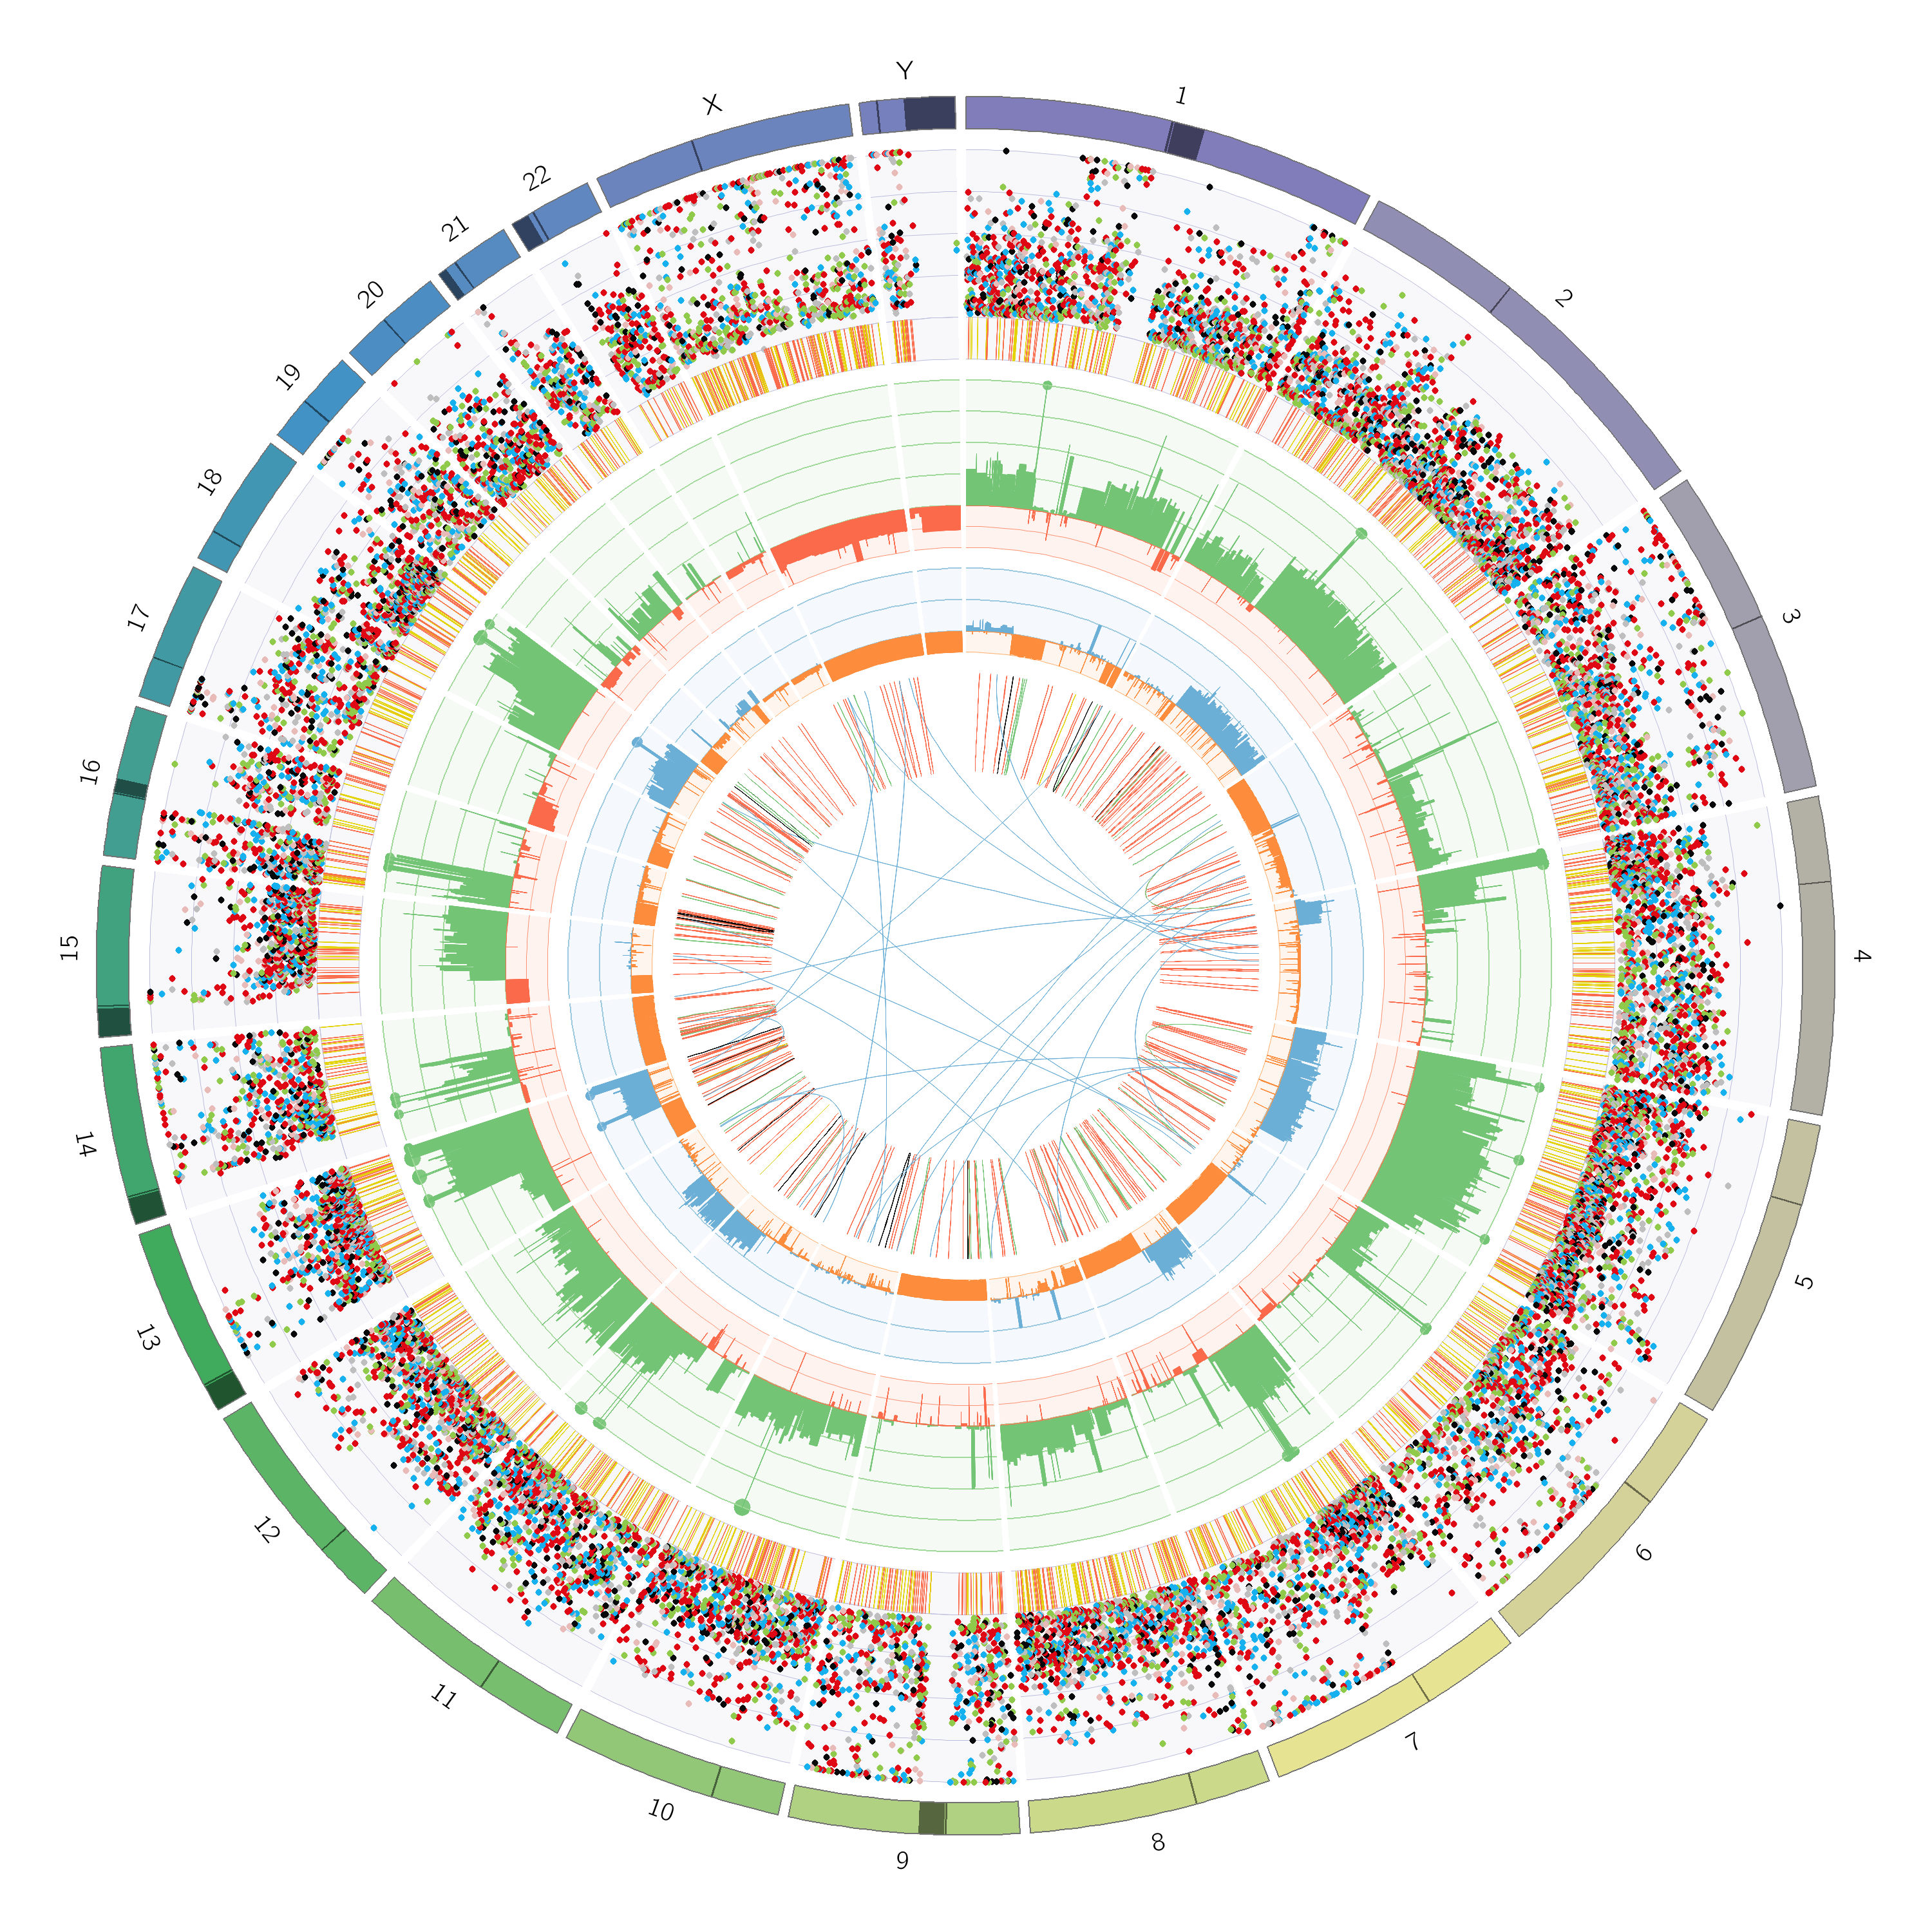
\includegraphics[width=.99\linewidth]{Figures/CASCADE/CA99/CA99-26.circos.png}
\caption[Circos plot of patient CA-A sample 26]{Circos plot of patient CA-A sample 26 with somatic structural variants with allele frequency $> 0.2$: outer first ring shows the canonical chromosomes with gaps (centromere, heterochromatin,...) highlighted as darker areas; second ring visualises all somatic SNVs corrected for tumour purity and scaled from 0 to 1, the colour representing the base change of SNV like in \protect\textcite{Alexandrov2013}; vertical lines directly under the SNVs symbolise InDels, with yellow for insertions and red for deletions; the third ring shows the total copy number alterations, with green showing a copy number gain and red a loss, dots at the outer border show a copy number greater than four; the last ring shows the minor copy number, with blue depicting a gain and orange a loss, this ring allows the detection of copy number neutral changes, like loss of heterozygosity; the center shows all structural variants: translocations in blue, deletions in red, insertions in yellow, tandem duplications in green and inversions in black.} \label{fig:ca99.26circos}
\end{figure}


\begin{figure}[!ht]
\centering
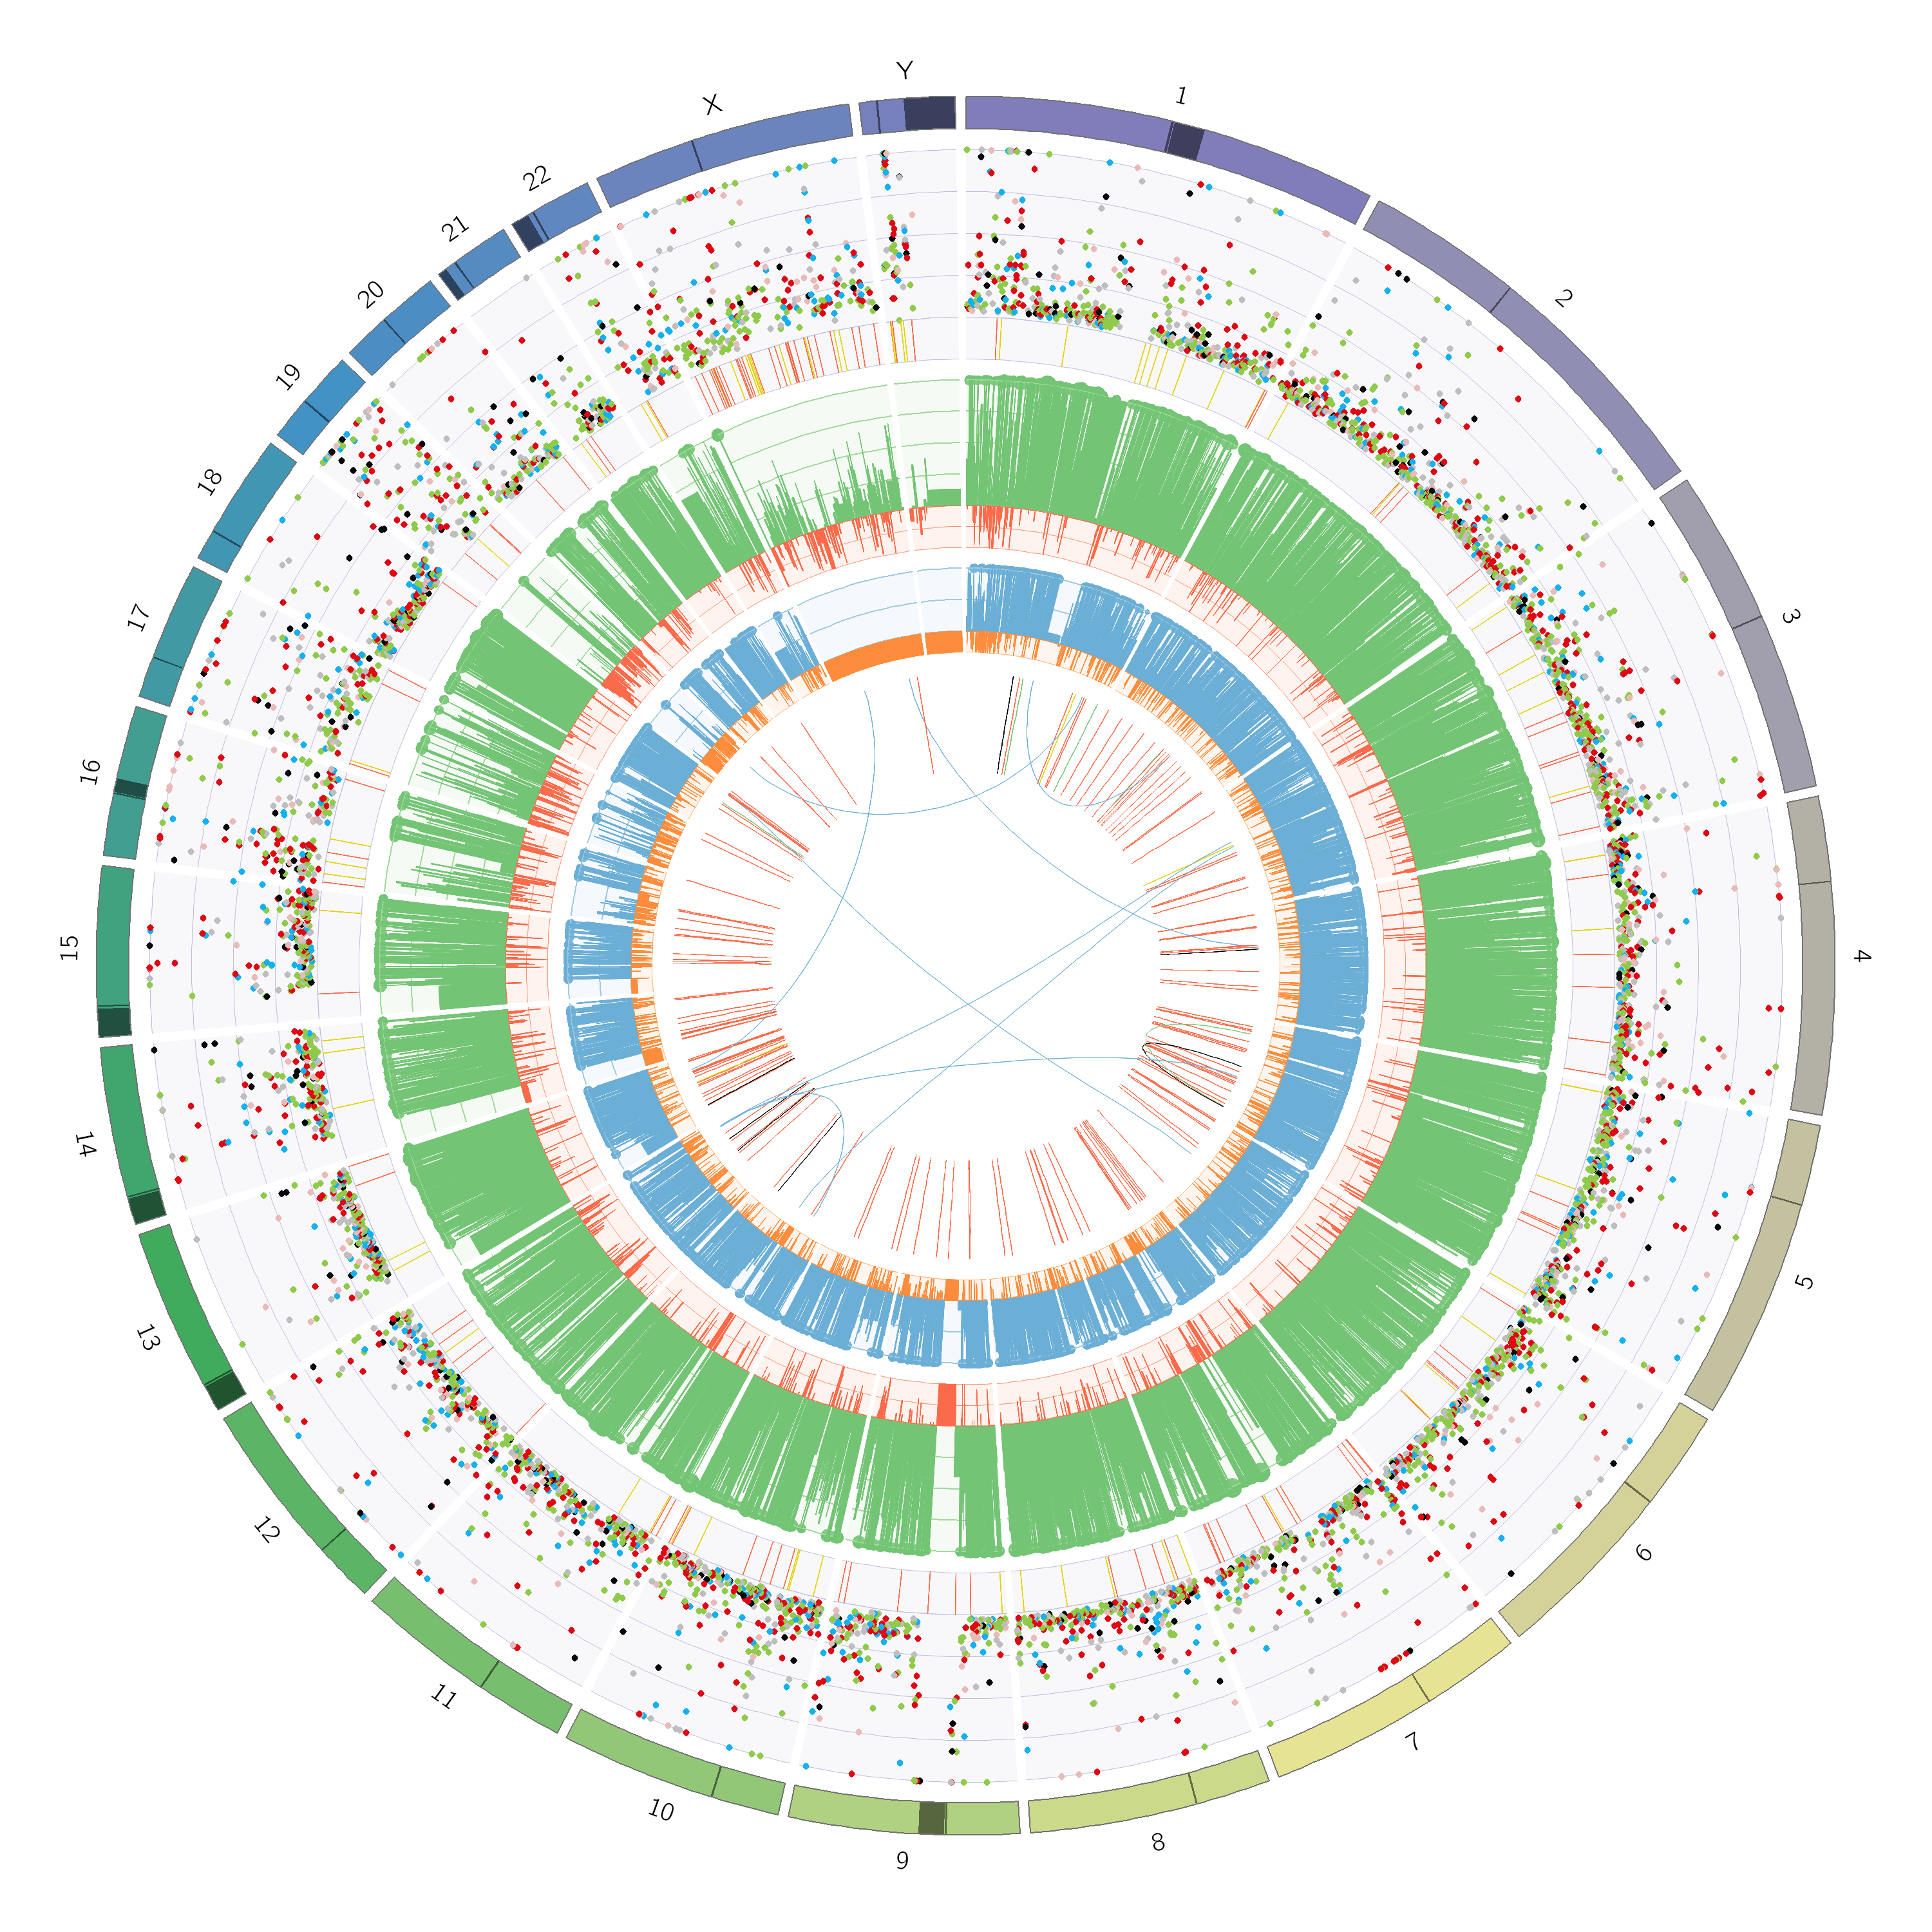
\includegraphics[width=.99\linewidth]{Figures/CASCADE/CA99/CA99-31.circos.png}
\caption[Circos plot of patient CA-A sample 31]{Circos plot of patient CA-A sample 31 with somatic structural variants with allele frequency $> 0.2$: outer first ring shows the canonical chromosomes with gaps (centromere, heterochromatin,...) highlighted as darker areas; second ring visualises all somatic SNVs corrected for tumour purity and scaled from 0 to 1, the colour representing the base change of SNV like in \protect\textcite{Alexandrov2013}; vertical lines directly under the SNVs symbolise InDels, with yellow for insertions and red for deletions; the third ring shows the total copy number alterations, with green showing a copy number gain and red a loss, dots at the outer border show a copy number greater than four; the last ring shows the minor copy number, with blue depicting a gain and orange a loss, this ring allows the detection of copy number neutral changes, like loss of heterozygosity; the center shows all structural variants: translocations in blue, deletions in red, insertions in yellow, tandem duplications in green and inversions in black.} \label{fig:ca99.31circos}
\end{figure}


\begin{figure}[!ht]
\centering
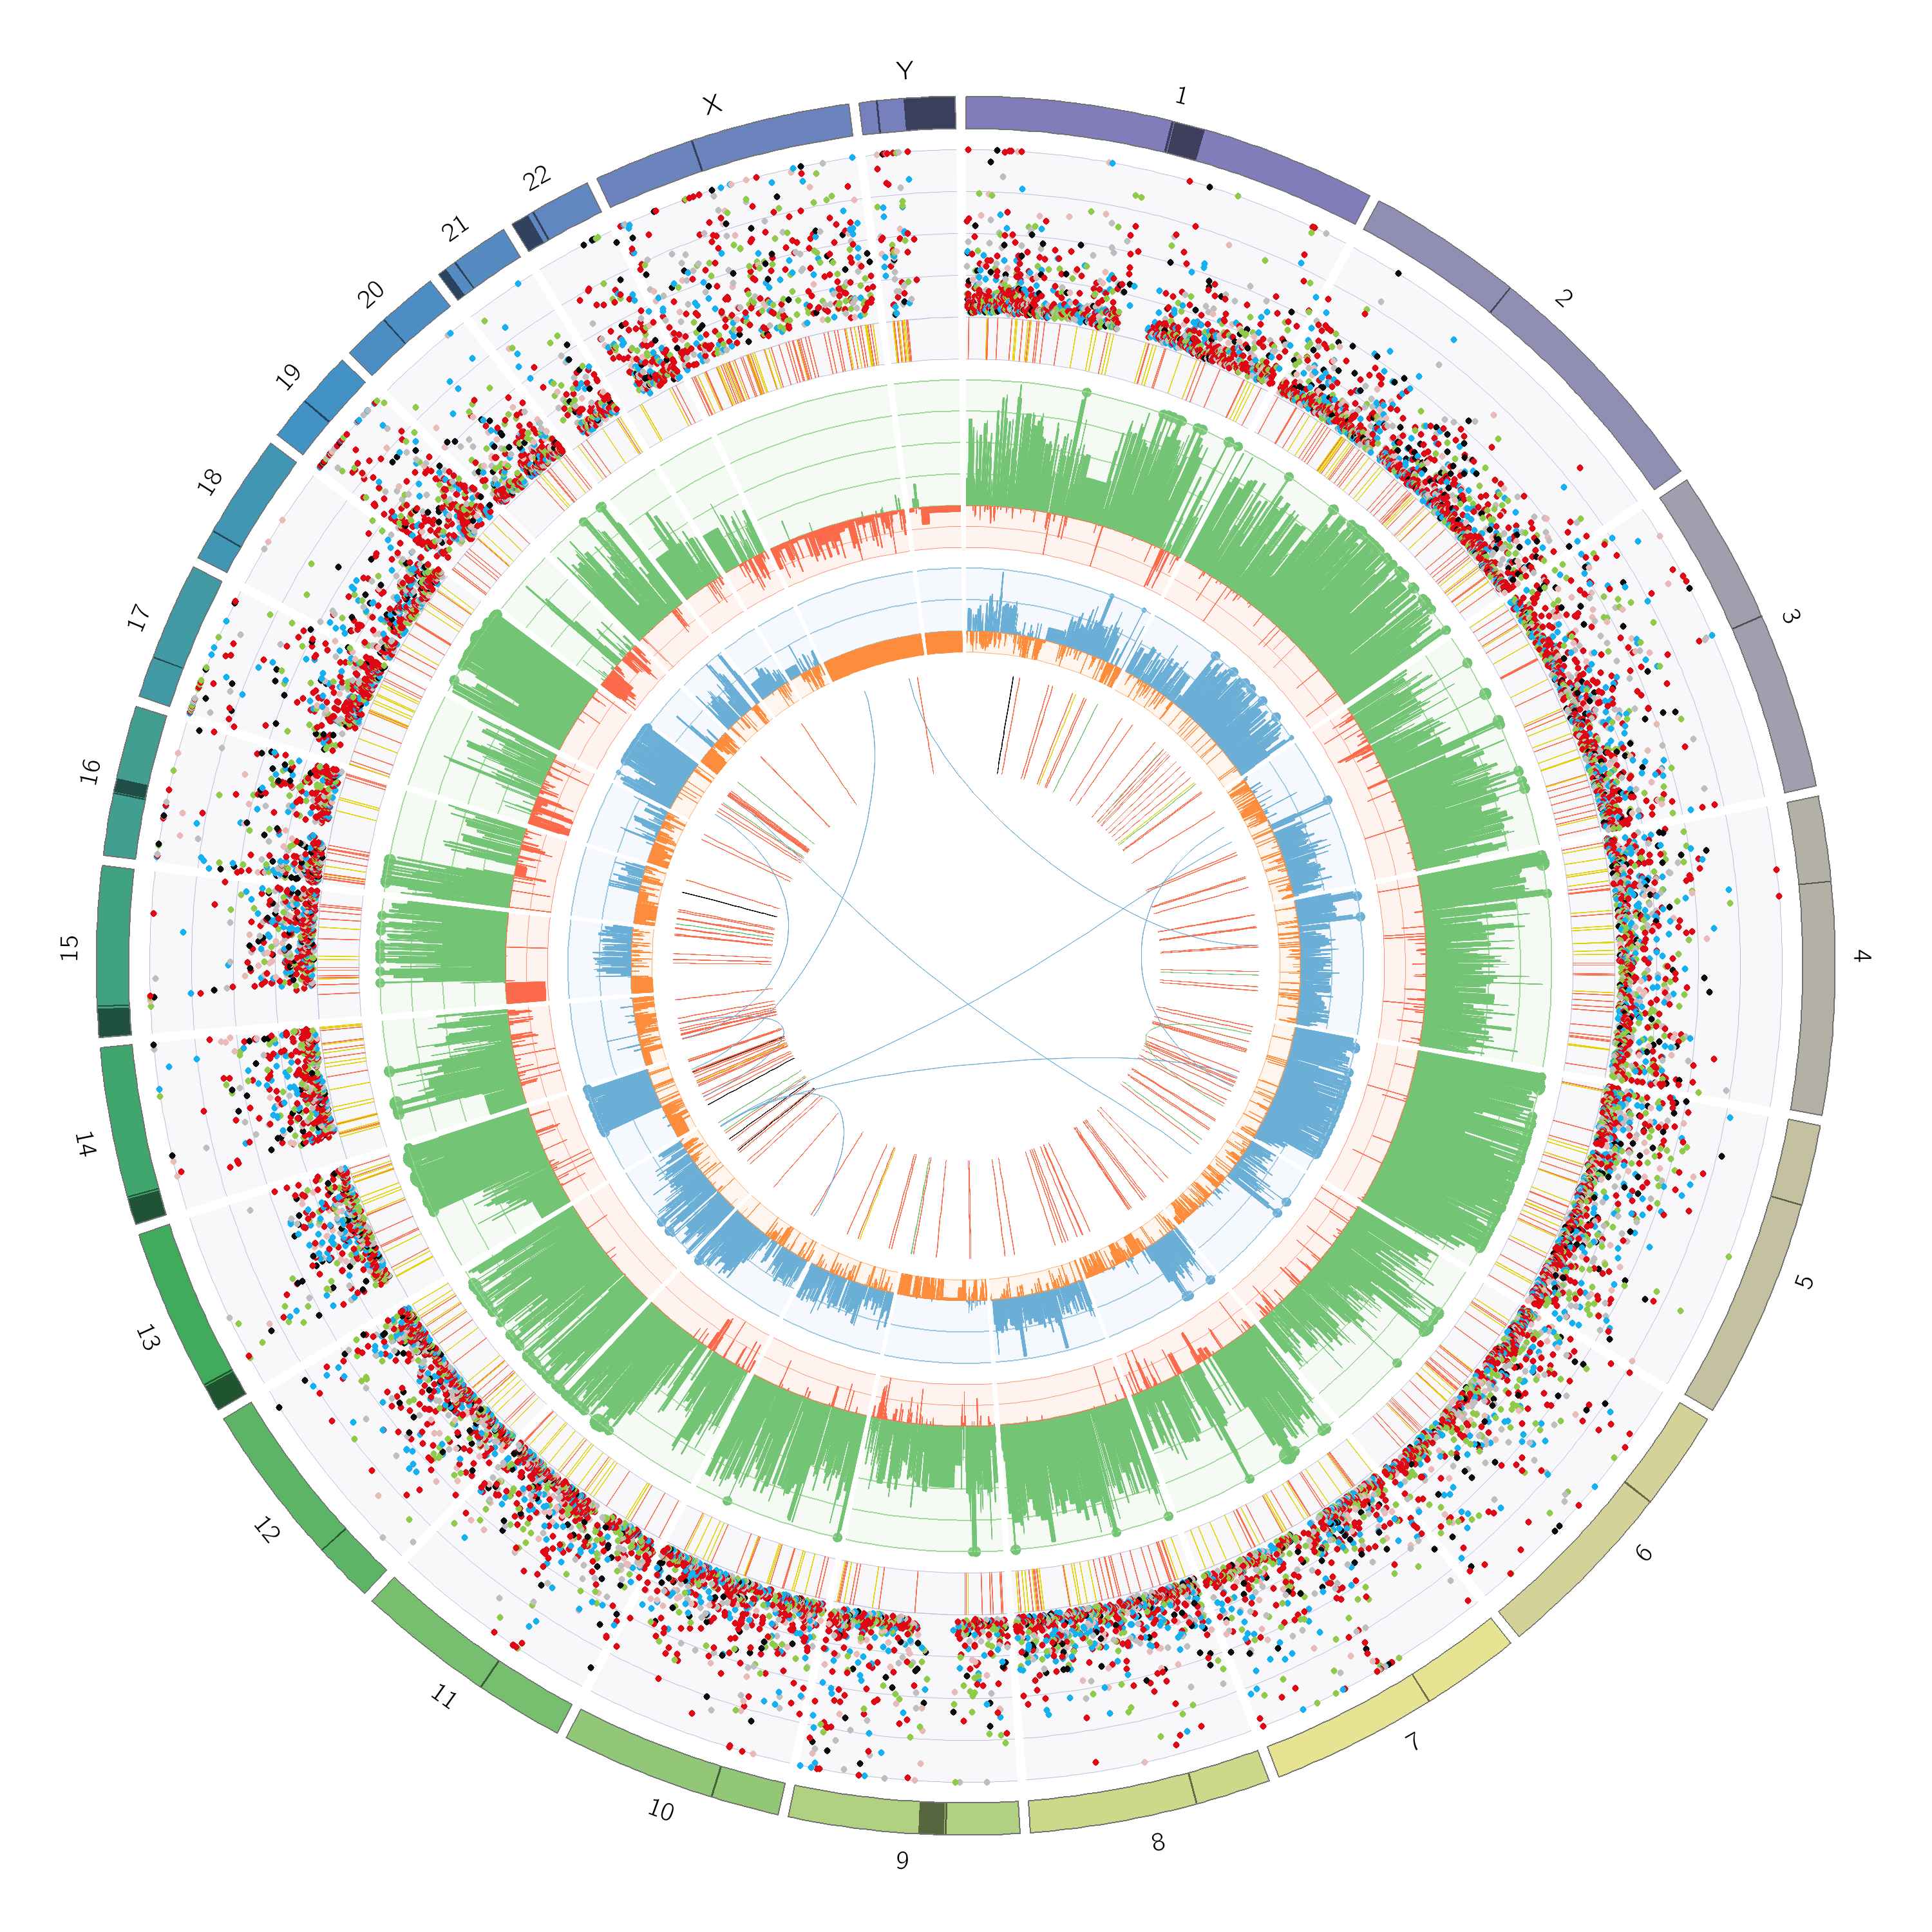
\includegraphics[width=.99\linewidth]{Figures/CASCADE/CA99/CA99-41.circos.png}
\caption[Circos plot of patient CA-A sample 41]{Circos plot of patient CA-A sample 41 with somatic structural variants with allele frequency $> 0.2$: outer first ring shows the canonical chromosomes with gaps (centromere, heterochromatin,...) highlighted as darker areas; second ring visualises all somatic SNVs corrected for tumour purity and scaled from 0 to 1, the colour representing the base change of SNV like in \protect\textcite{Alexandrov2013}; vertical lines directly under the SNVs symbolise InDels, with yellow for insertions and red for deletions; the third ring shows the total copy number alterations, with green showing a copy number gain and red a loss, dots at the outer border show a copy number greater than four; the last ring shows the minor copy number, with blue depicting a gain and orange a loss, this ring allows the detection of copy number neutral changes, like loss of heterozygosity; the center shows all structural variants: translocations in blue, deletions in red, insertions in yellow, tandem duplications in green and inversions in black.} \label{fig:ca99.41circos}
\end{figure}



\begin{figure}[!ht]
\centering
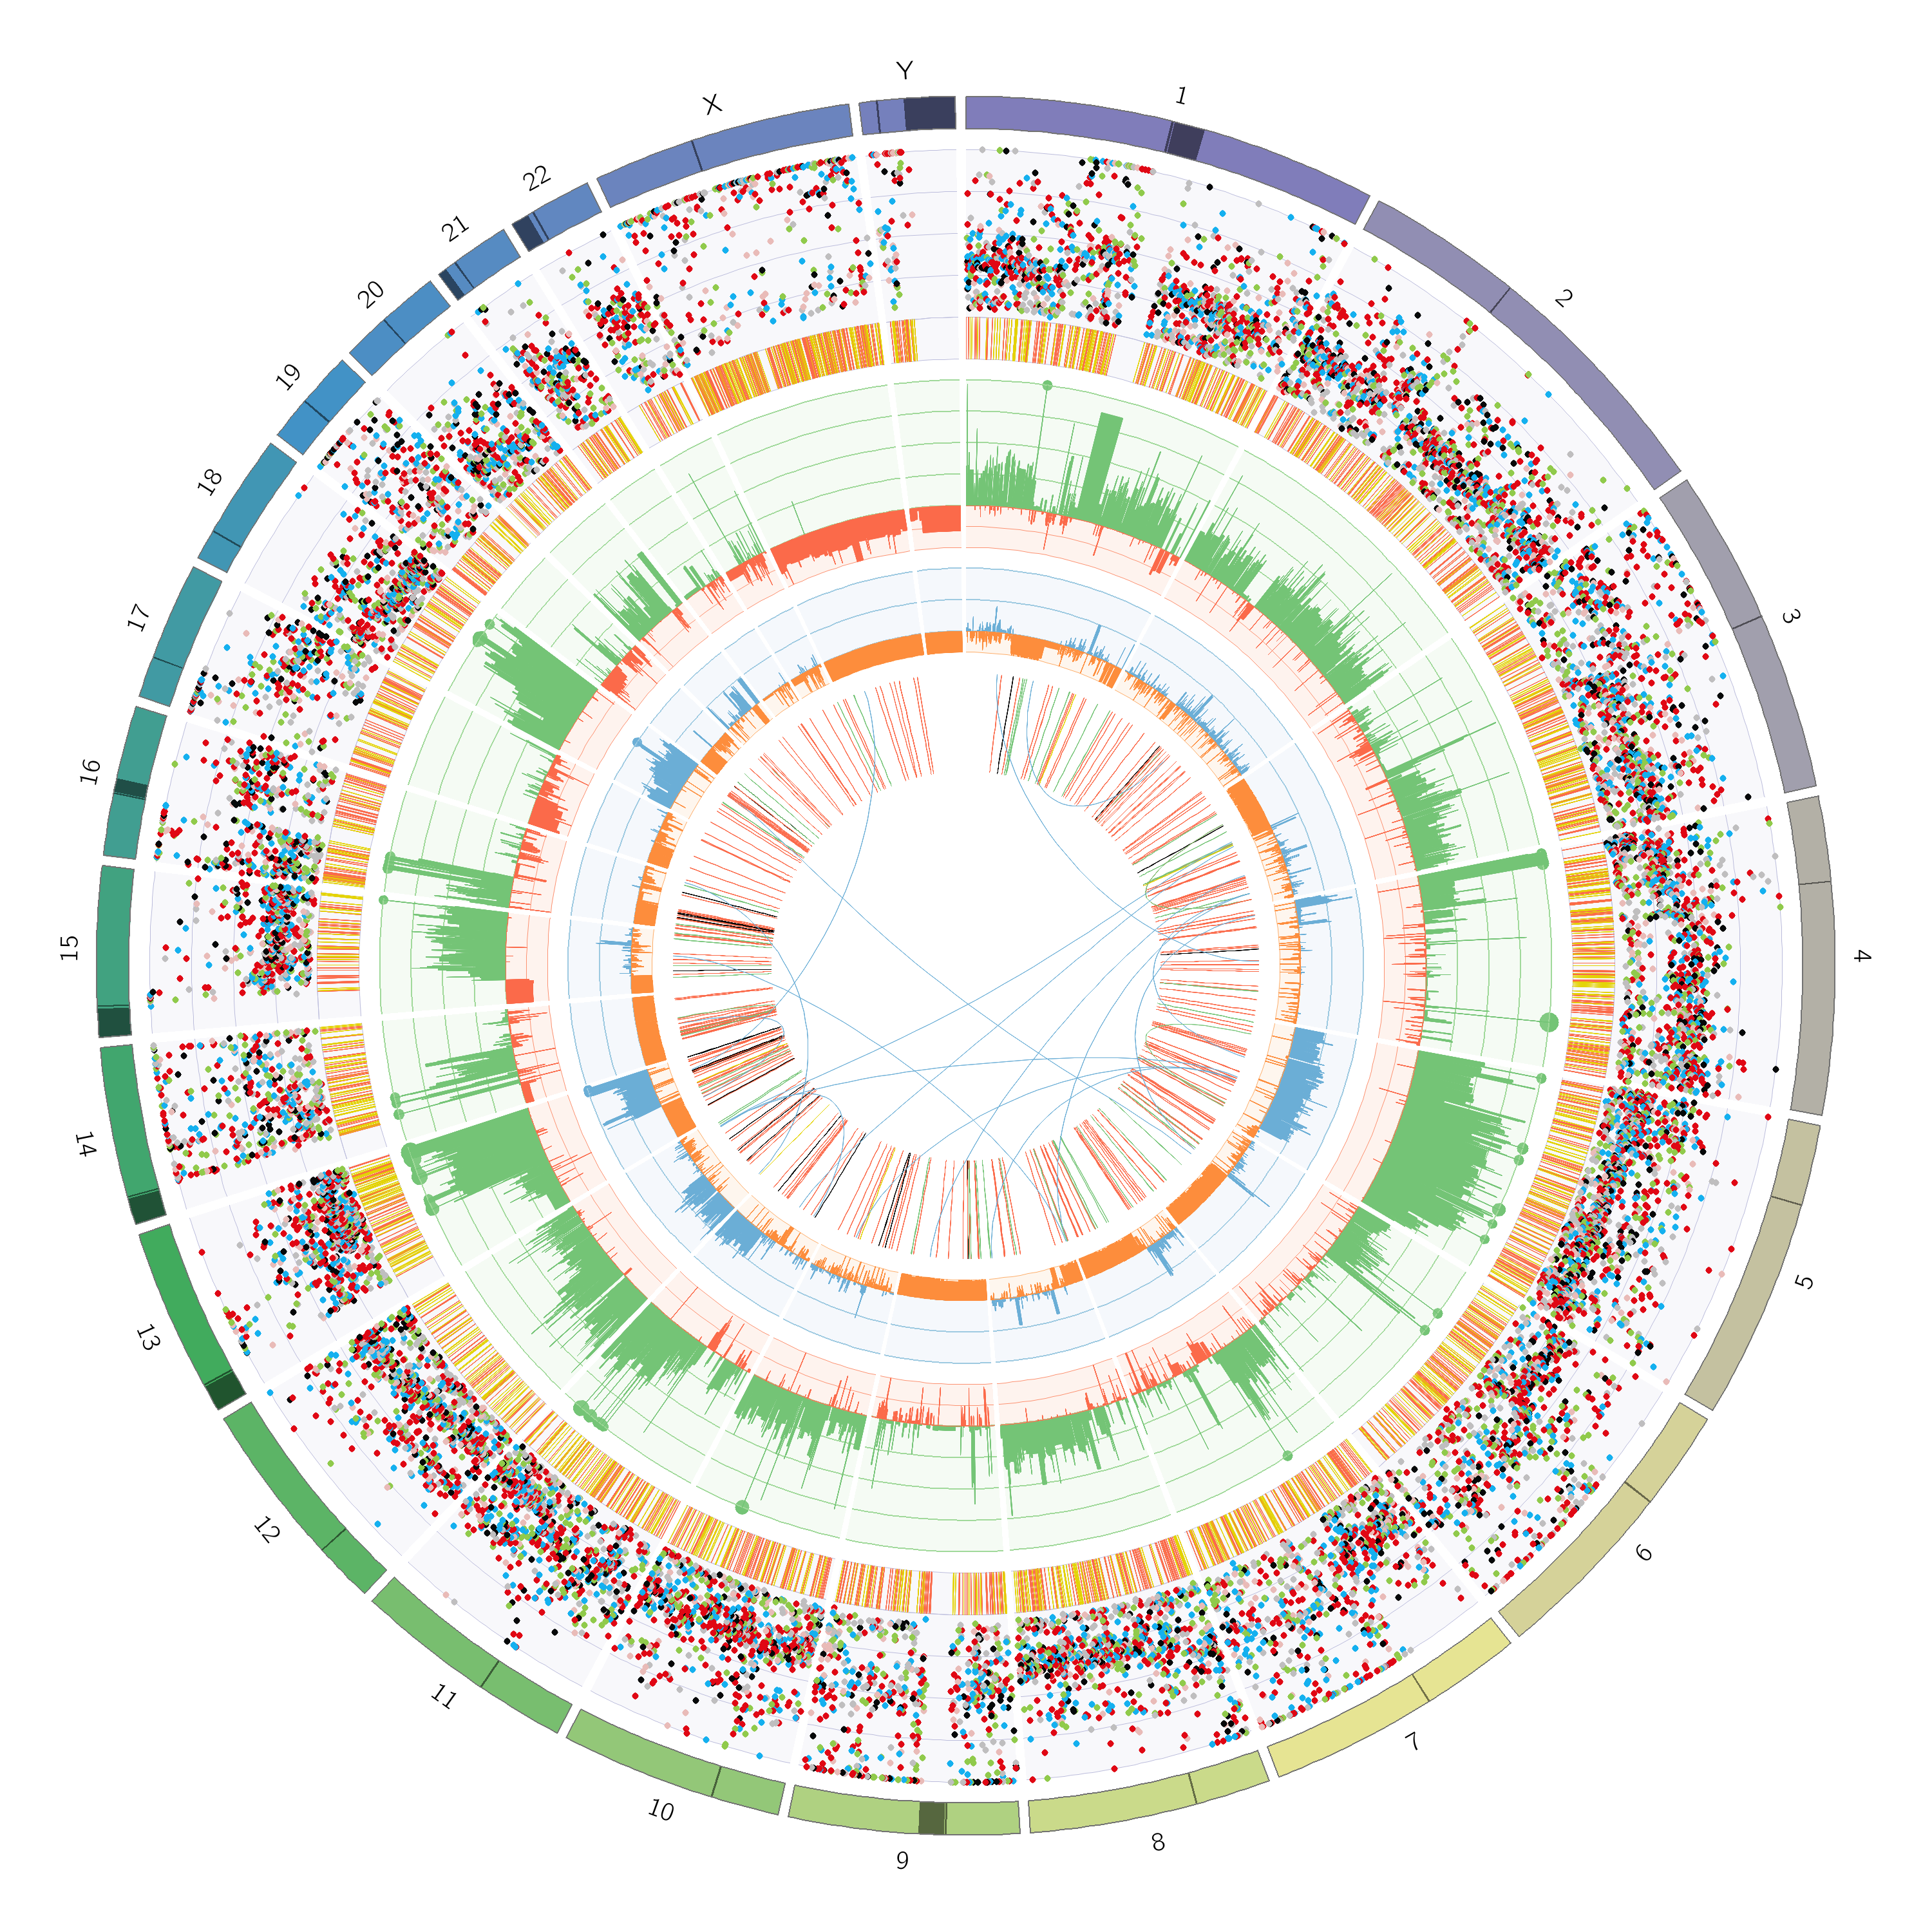
\includegraphics[width=.99\linewidth]{Figures/CASCADE/CA99/CA99-47.circos.png}
\caption[Circos plot of patient CA-A sample 47]{Circos plot of patient CA-A sample 47 with somatic structural variants with allele frequency $> 0.2$: outer first ring shows the canonical chromosomes with gaps (centromere, heterochromatin,...) highlighted as darker areas; second ring visualises all somatic SNVs corrected for tumour purity and scaled from 0 to 1, the colour representing the base change of SNV like in \protect\textcite{Alexandrov2013}; vertical lines directly under the SNVs symbolise InDels, with yellow for insertions and red for deletions; the third ring shows the total copy number alterations, with green showing a copy number gain and red a loss, dots at the outer border show a copy number greater than four; the last ring shows the minor copy number, with blue depicting a gain and orange a loss, this ring allows the detection of copy number neutral changes, like loss of heterozygosity; the center shows all structural variants: translocations in blue, deletions in red, insertions in yellow, tandem duplications in green and inversions in black.} \label{fig:ca99.47circos}
\end{figure}



\begin{figure}[!ht]
\centering
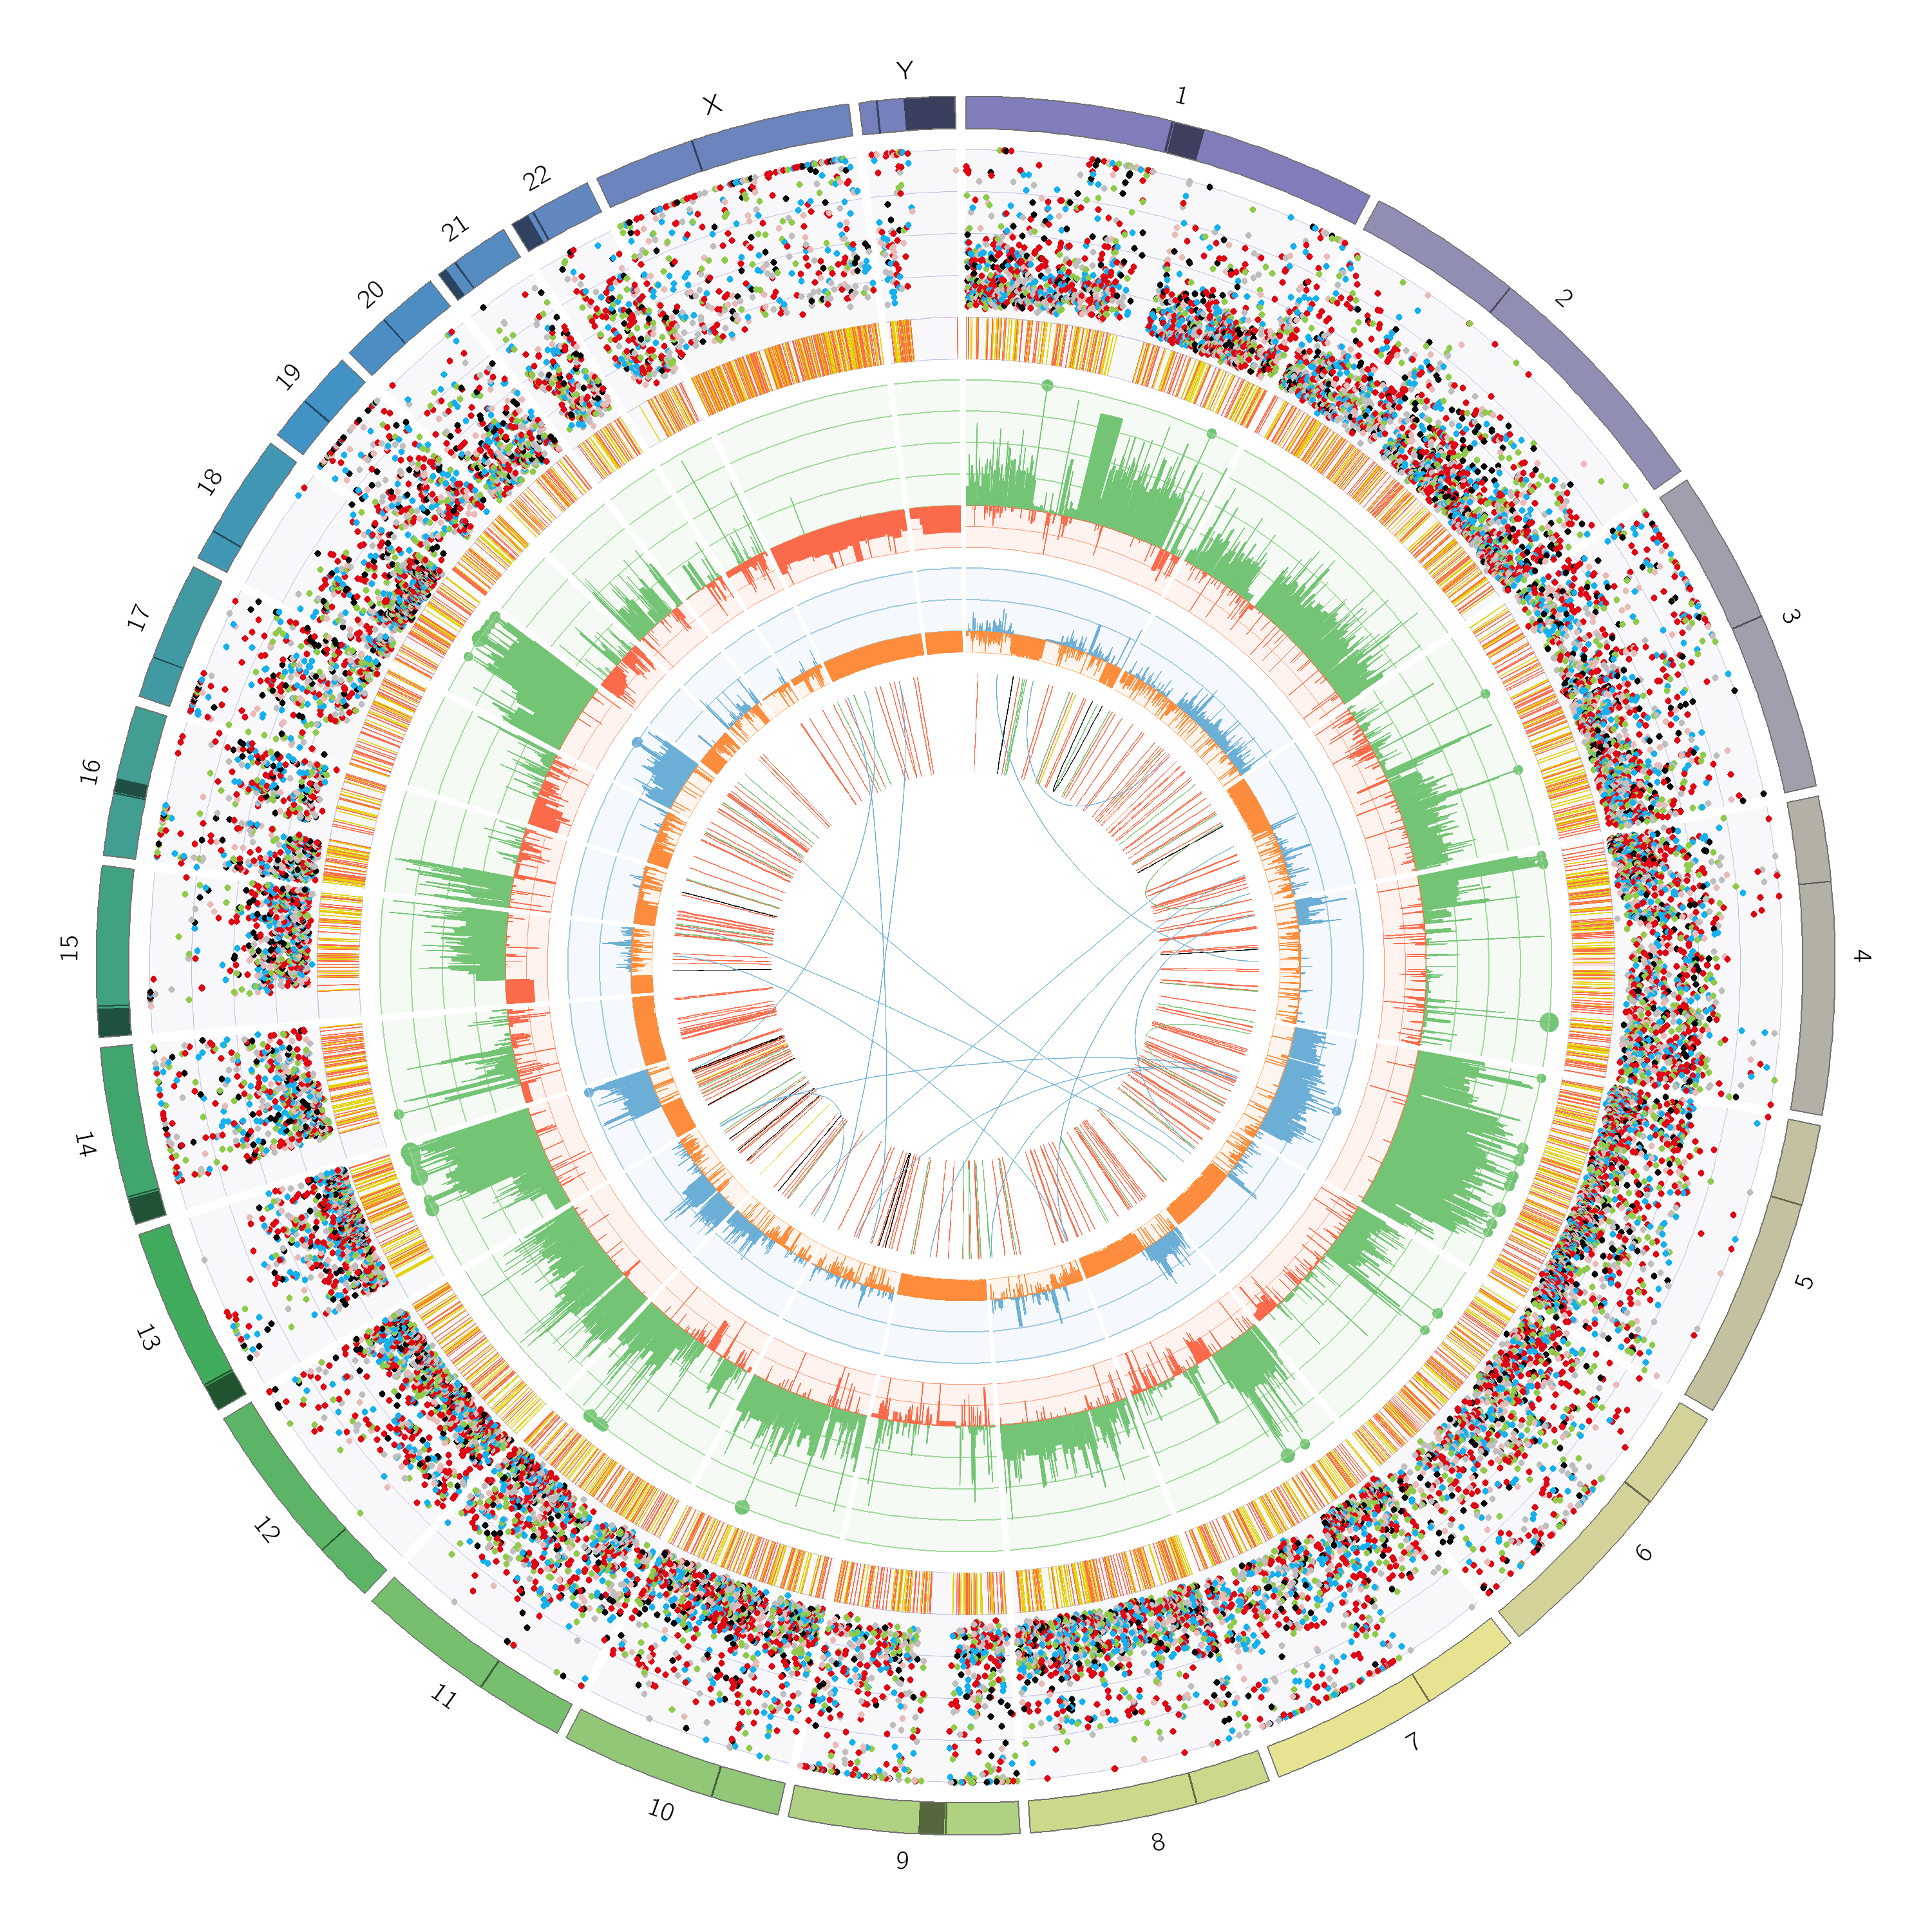
\includegraphics[width=.99\linewidth]{Figures/CASCADE/CA99/CA99-55.circos.png}
\caption[Circos plot of patient CA-A sample 55]{Circos plot of patient CA-A sample 55 with somatic structural variants with allele frequency $> 0.2$: outer first ring shows the canonical chromosomes with gaps (centromere, heterochromatin,...) highlighted as darker areas; second ring visualises all somatic SNVs corrected for tumour purity and scaled from 0 to 1, the colour representing the base change of SNV like in \protect\textcite{Alexandrov2013}; vertical lines directly under the SNVs symbolise InDels, with yellow for insertions and red for deletions; the third ring shows the total copy number alterations, with green showing a copy number gain and red a loss, dots at the outer border show a copy number greater than four; the last ring shows the minor copy number, with blue depicting a gain and orange a loss, this ring allows the detection of copy number neutral changes, like loss of heterozygosity; the center shows all structural variants: translocations in blue, deletions in red, insertions in yellow, tandem duplications in green and inversions in black.} \label{fig:ca99.55circos}
\end{figure}



\begin{figure}[!ht]
\centering
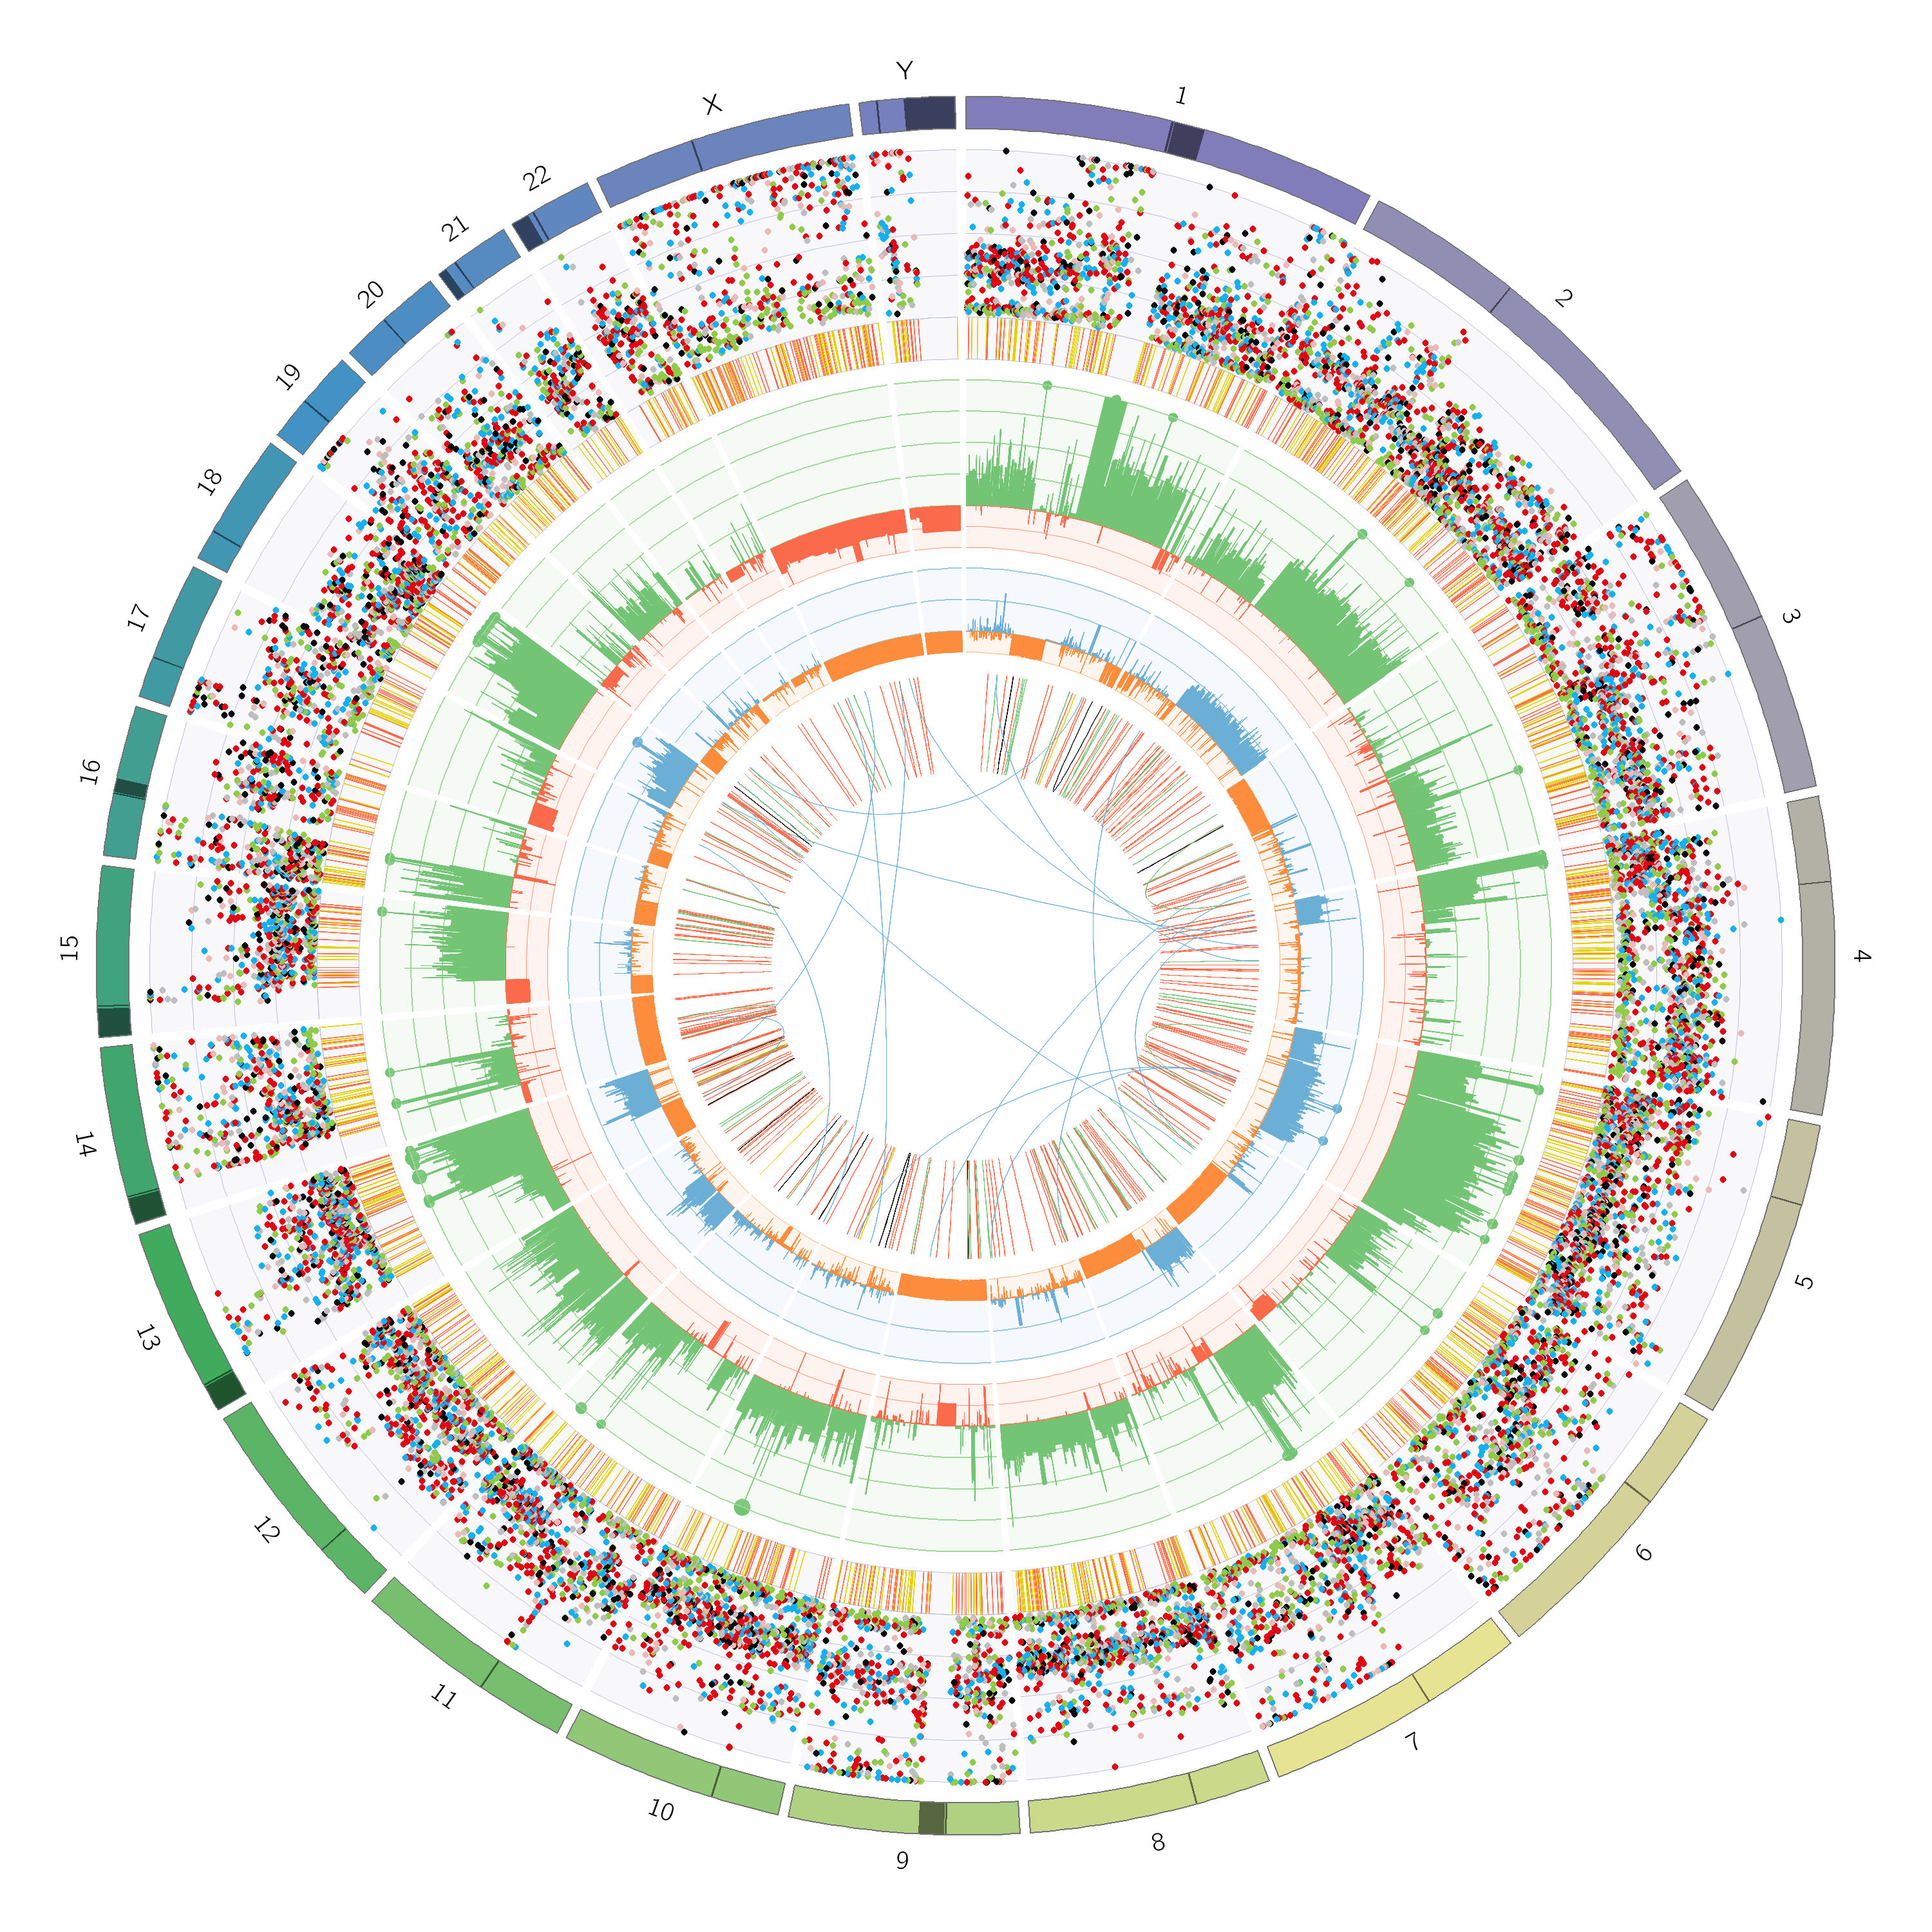
\includegraphics[width=.99\linewidth]{Figures/CASCADE/CA99/CA99-57.circos.png}
\caption[Circos plot of patient CA-A sample 57]{Circos plot of patient CA-A sample 57 with somatic structural variants with allele frequency $> 0.2$: outer first ring shows the canonical chromosomes with gaps (centromere, heterochromatin,...) highlighted as darker areas; second ring visualises all somatic SNVs corrected for tumour purity and scaled from 0 to 1, the colour representing the base change of SNV like in \protect\textcite{Alexandrov2013}; vertical lines directly under the SNVs symbolise InDels, with yellow for insertions and red for deletions; the third ring shows the total copy number alterations, with green showing a copy number gain and red a loss, dots at the outer border show a copy number greater than four; the last ring shows the minor copy number, with blue depicting a gain and orange a loss, this ring allows the detection of copy number neutral changes, like loss of heterozygosity; the center shows all structural variants: translocations in blue, deletions in red, insertions in yellow, tandem duplications in green and inversions in black.} \label{fig:ca99.57circos}
\end{figure}


\begin{figure}[!ht]
\centering
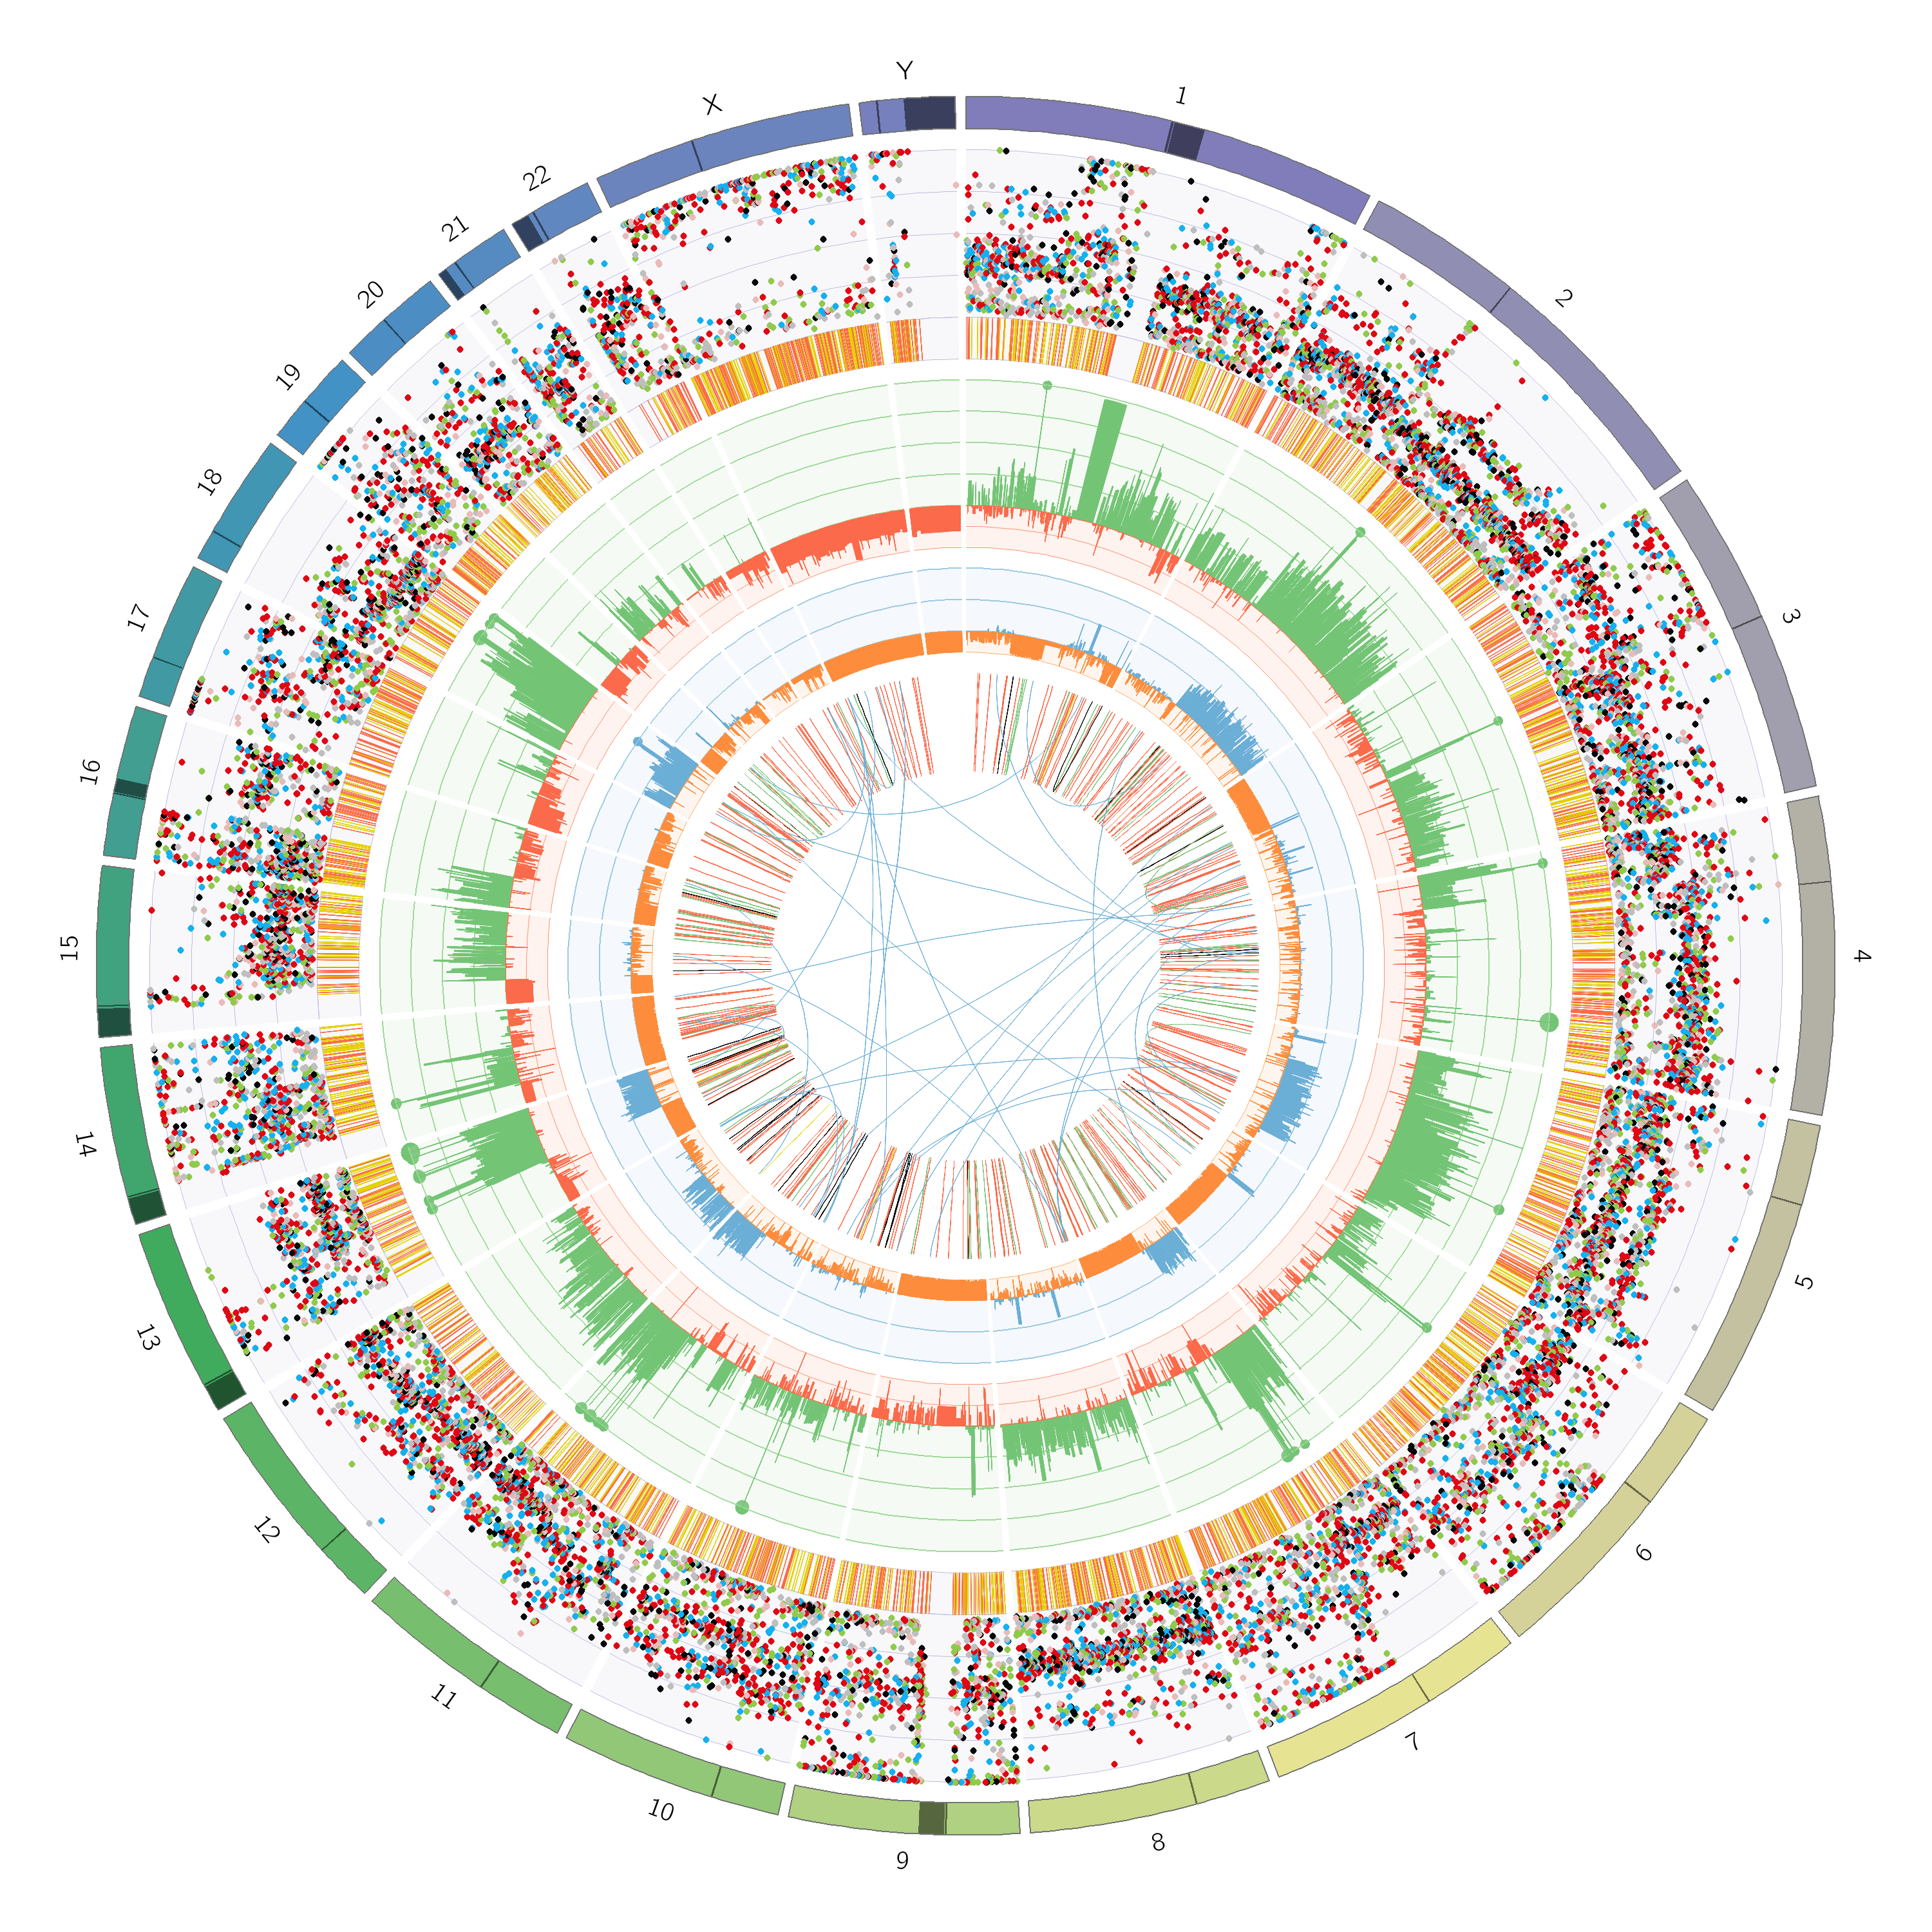
\includegraphics[width=.99\linewidth]{Figures/CASCADE/CA99/CA99-59.circos.png}
\caption[Circos plot of patient CA-A sample 59]{Circos plot of patient CA-A sample 59 with somatic structural variants with allele frequency $> 0.2$: outer first ring shows the canonical chromosomes with gaps (centromere, heterochromatin,...) highlighted as darker areas; second ring visualises all somatic SNVs corrected for tumour purity and scaled from 0 to 1, the colour representing the base change of SNV like in \protect\textcite{Alexandrov2013}; vertical lines directly under the SNVs symbolise InDels, with yellow for insertions and red for deletions; the third ring shows the total copy number alterations, with green showing a copy number gain and red a loss, dots at the outer border show a copy number greater than four; the last ring shows the minor copy number, with blue depicting a gain and orange a loss, this ring allows the detection of copy number neutral changes, like loss of heterozygosity; the center shows all structural variants: translocations in blue, deletions in red, insertions in yellow, tandem duplications in green and inversions in black.} \label{fig:ca99.59circos}
\end{figure}

\cleardoublepage

\subsection{Patient CA-I}

\begin{figure}[ht]
\centering
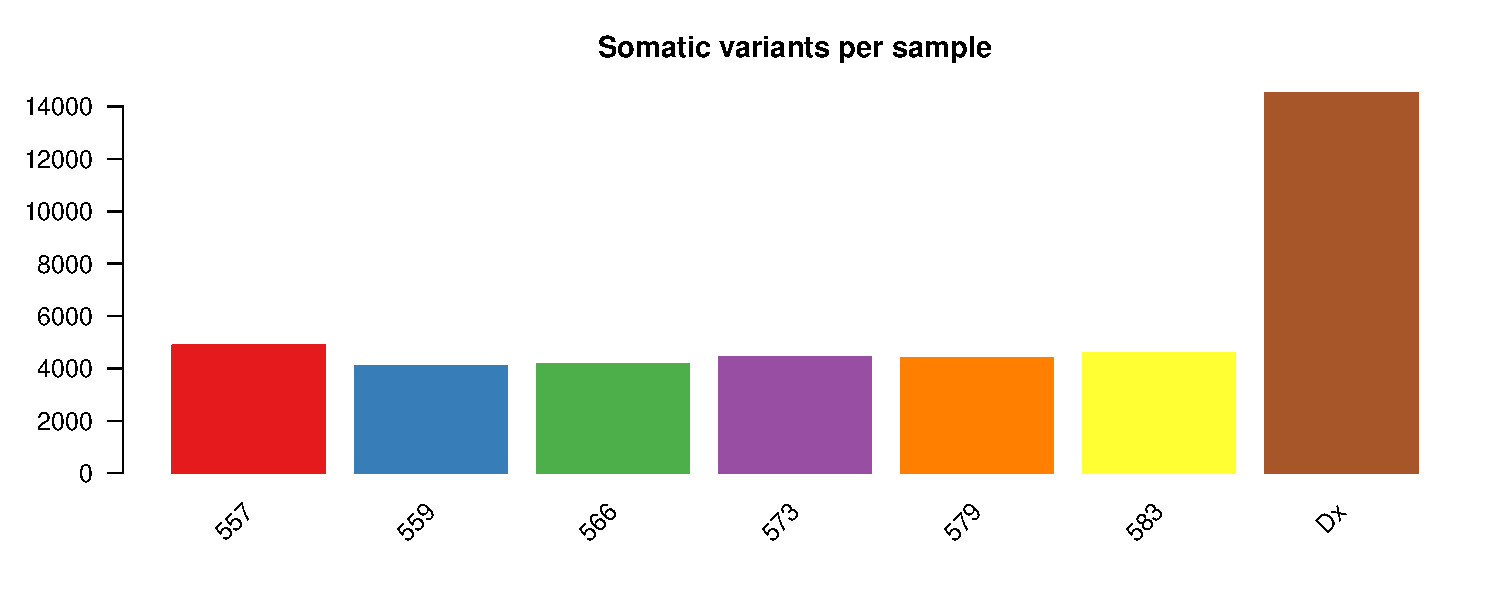
\includegraphics[width=.99\linewidth]{Figures/CASCADE/CA51/CA51numVars.pdf}
\caption[Number of somatic variants per sample in patient CA-I]{Number of high confidence somatic variants per sample in patient CA-I; variants were called with the Strelka2Pass workflow and retricted to \emph{PASS} only} \label{fig:ca51numVars}
\end{figure}

\begin{figure}[ht]
\centering
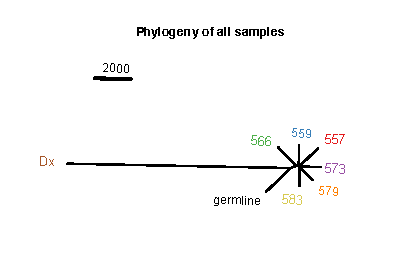
\includegraphics[width=.99\linewidth]{Figures/CASCADE/CA51/CA51phyloWithDx.pdf}
\caption[Phylogeny of samples from patient CA-I with diagnostic sample]{Phylogeny of samples from patient CA-I with diagnostic sample} \label{fig:ca51phyloWithDx}
\end{figure}




\begin{figure}[ht]
\centering
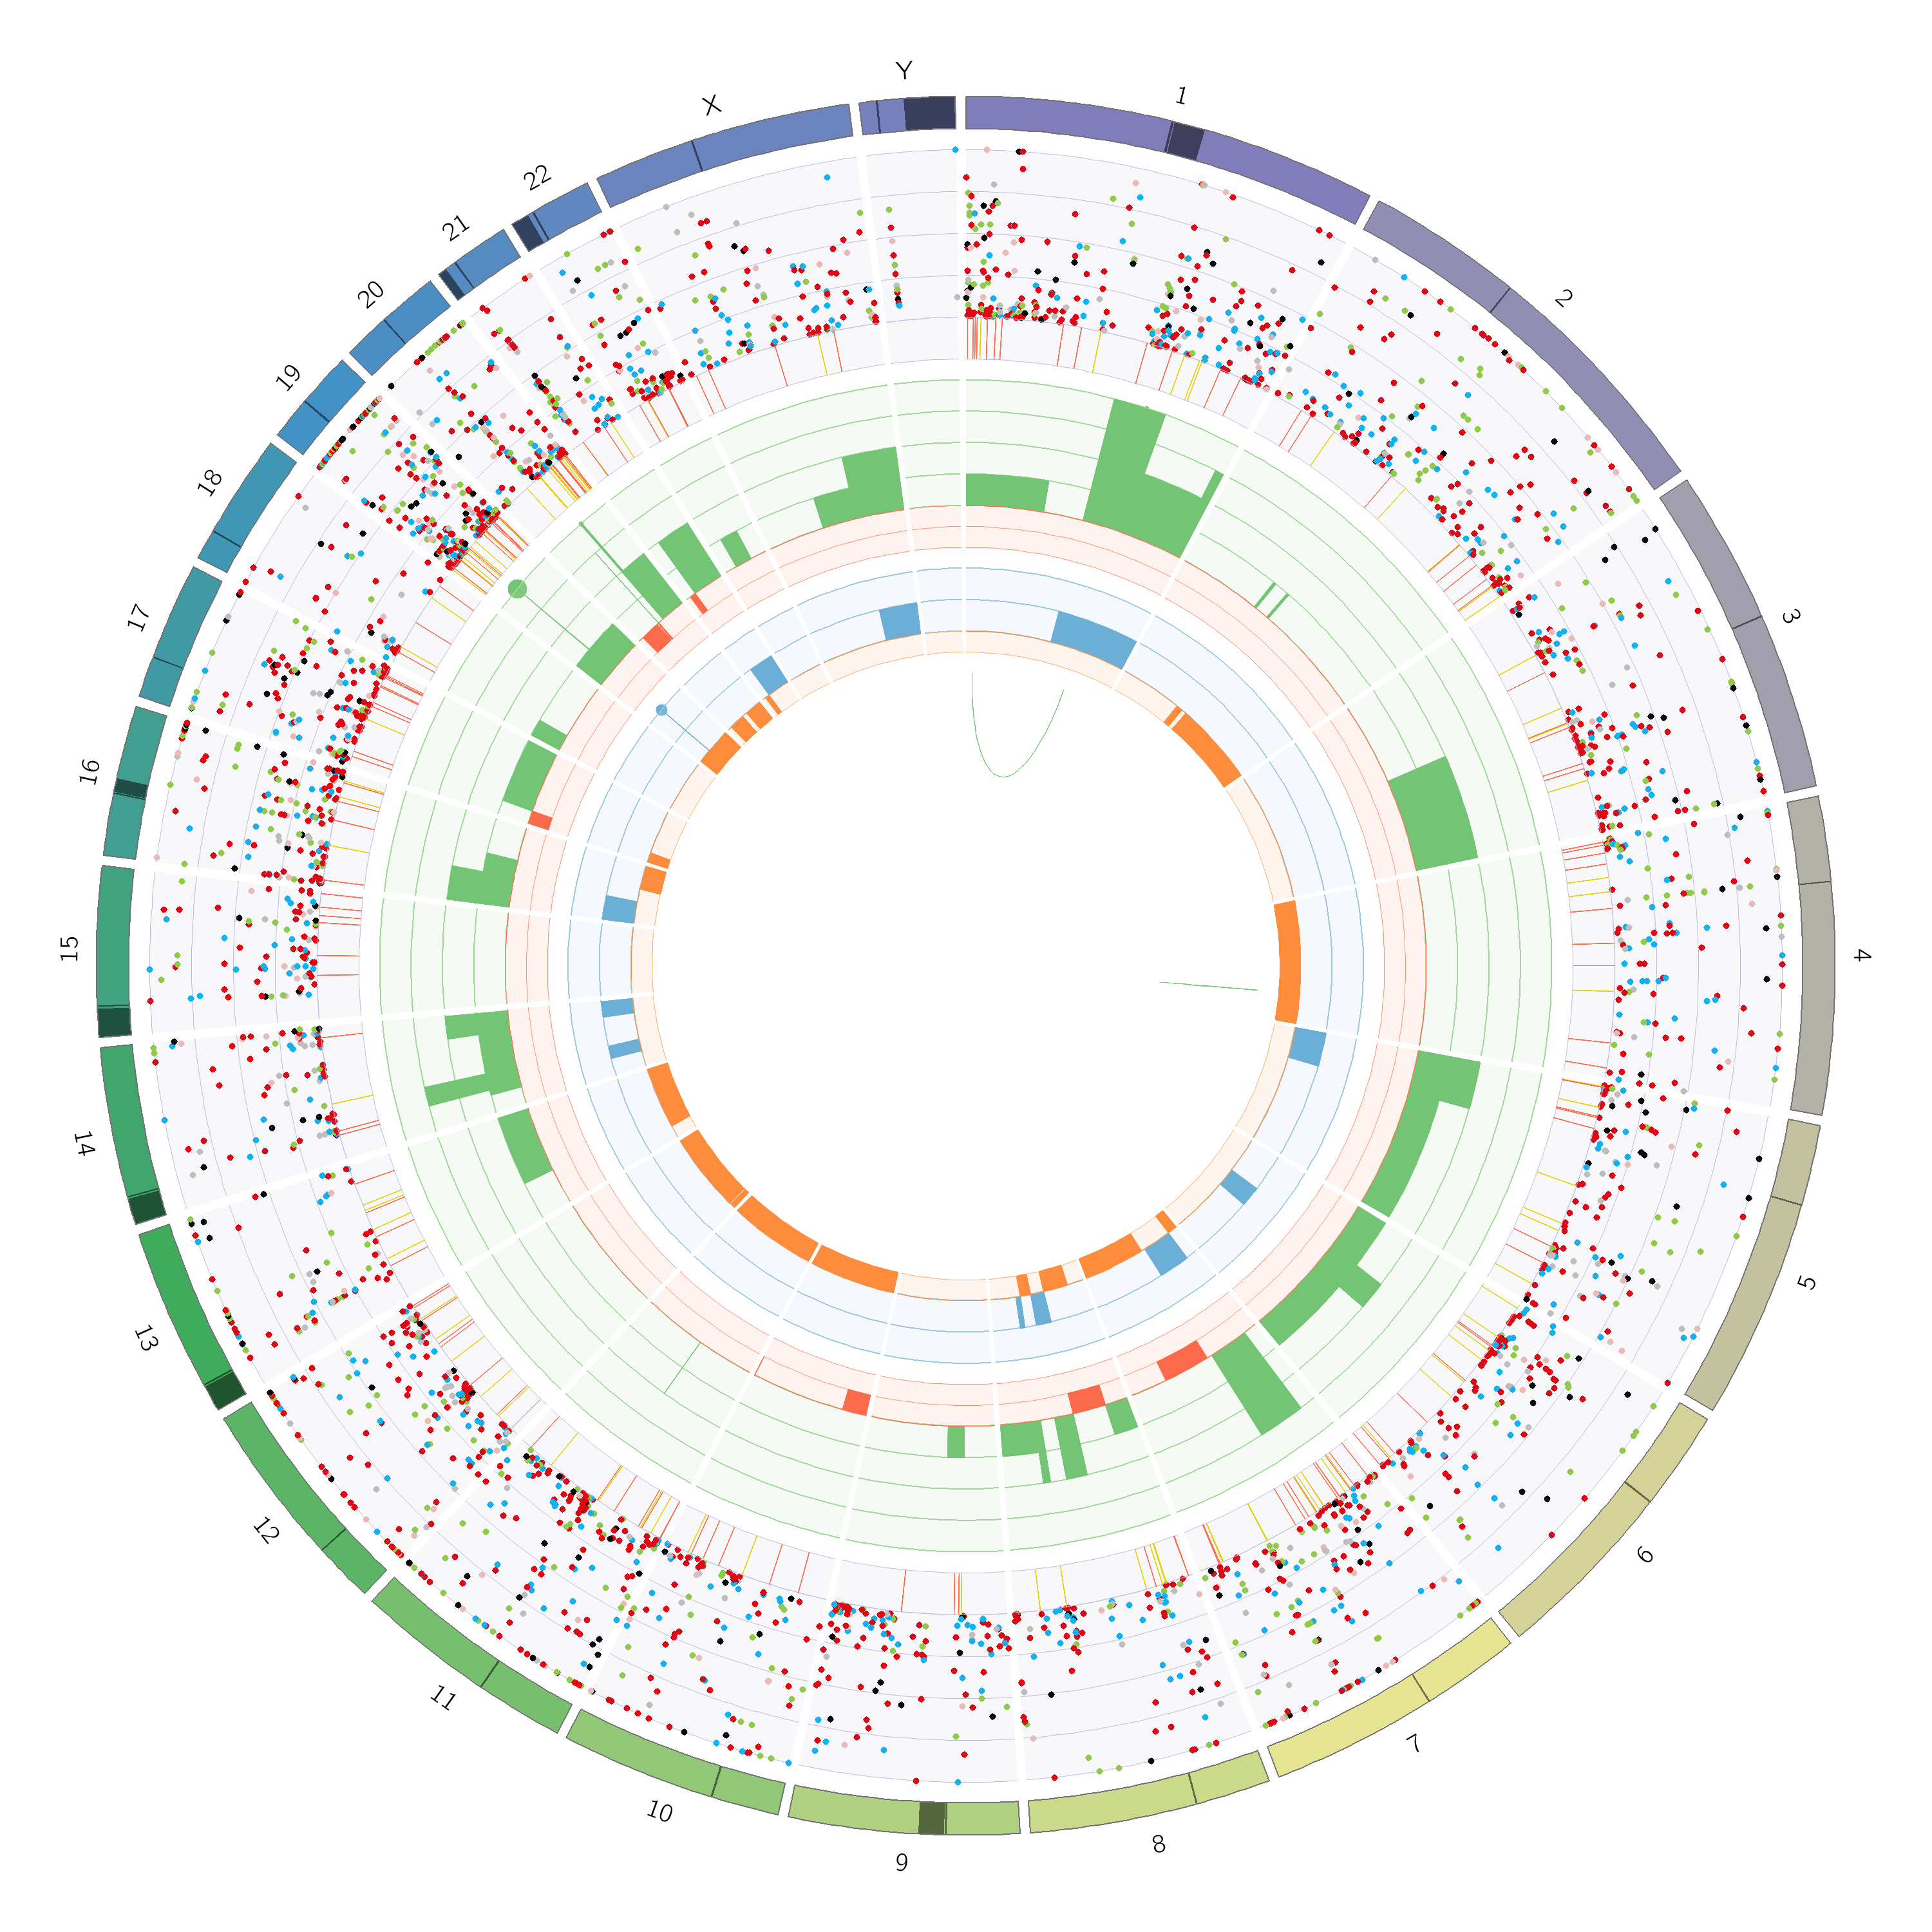
\includegraphics[width=.99\linewidth]{Figures/CASCADE/CA51/CA51-559.circos.png}
\caption[Circos plot of patient CA-I sample 559]{Circos plot of patient CA-I sample 559 with somatic structural variants with allele frequency $> 0.2$: outer first ring shows the canonical chromosomes with gaps (centromere, heterochromatin,...) highlighted as darker areas; second ring visualises all somatic SNVs corrected for tumour purity and scaled from 0 to 1, the colour representing the base change of SNV like in \protect\textcite{Alexandrov2013}; vertical lines directly under the SNVs symbolise InDels, with yellow for insertions and red for deletions; the third ring shows the total copy number alterations, with green showing a copy number gain and red a loss, dots at the outer border show a copy number greater than four; the last ring shows the minor copy number, with blue depicting a gain and orange a loss, this ring allows the detection of copy number neutral changes, like loss of heterozygosity; the center shows all structural variants: translocations in blue, deletions in red, insertions in yellow, tandem duplications in green and inversions in black.} \label{fig:ca51.559circos}
\end{figure}

\begin{figure}[ht]
\centering
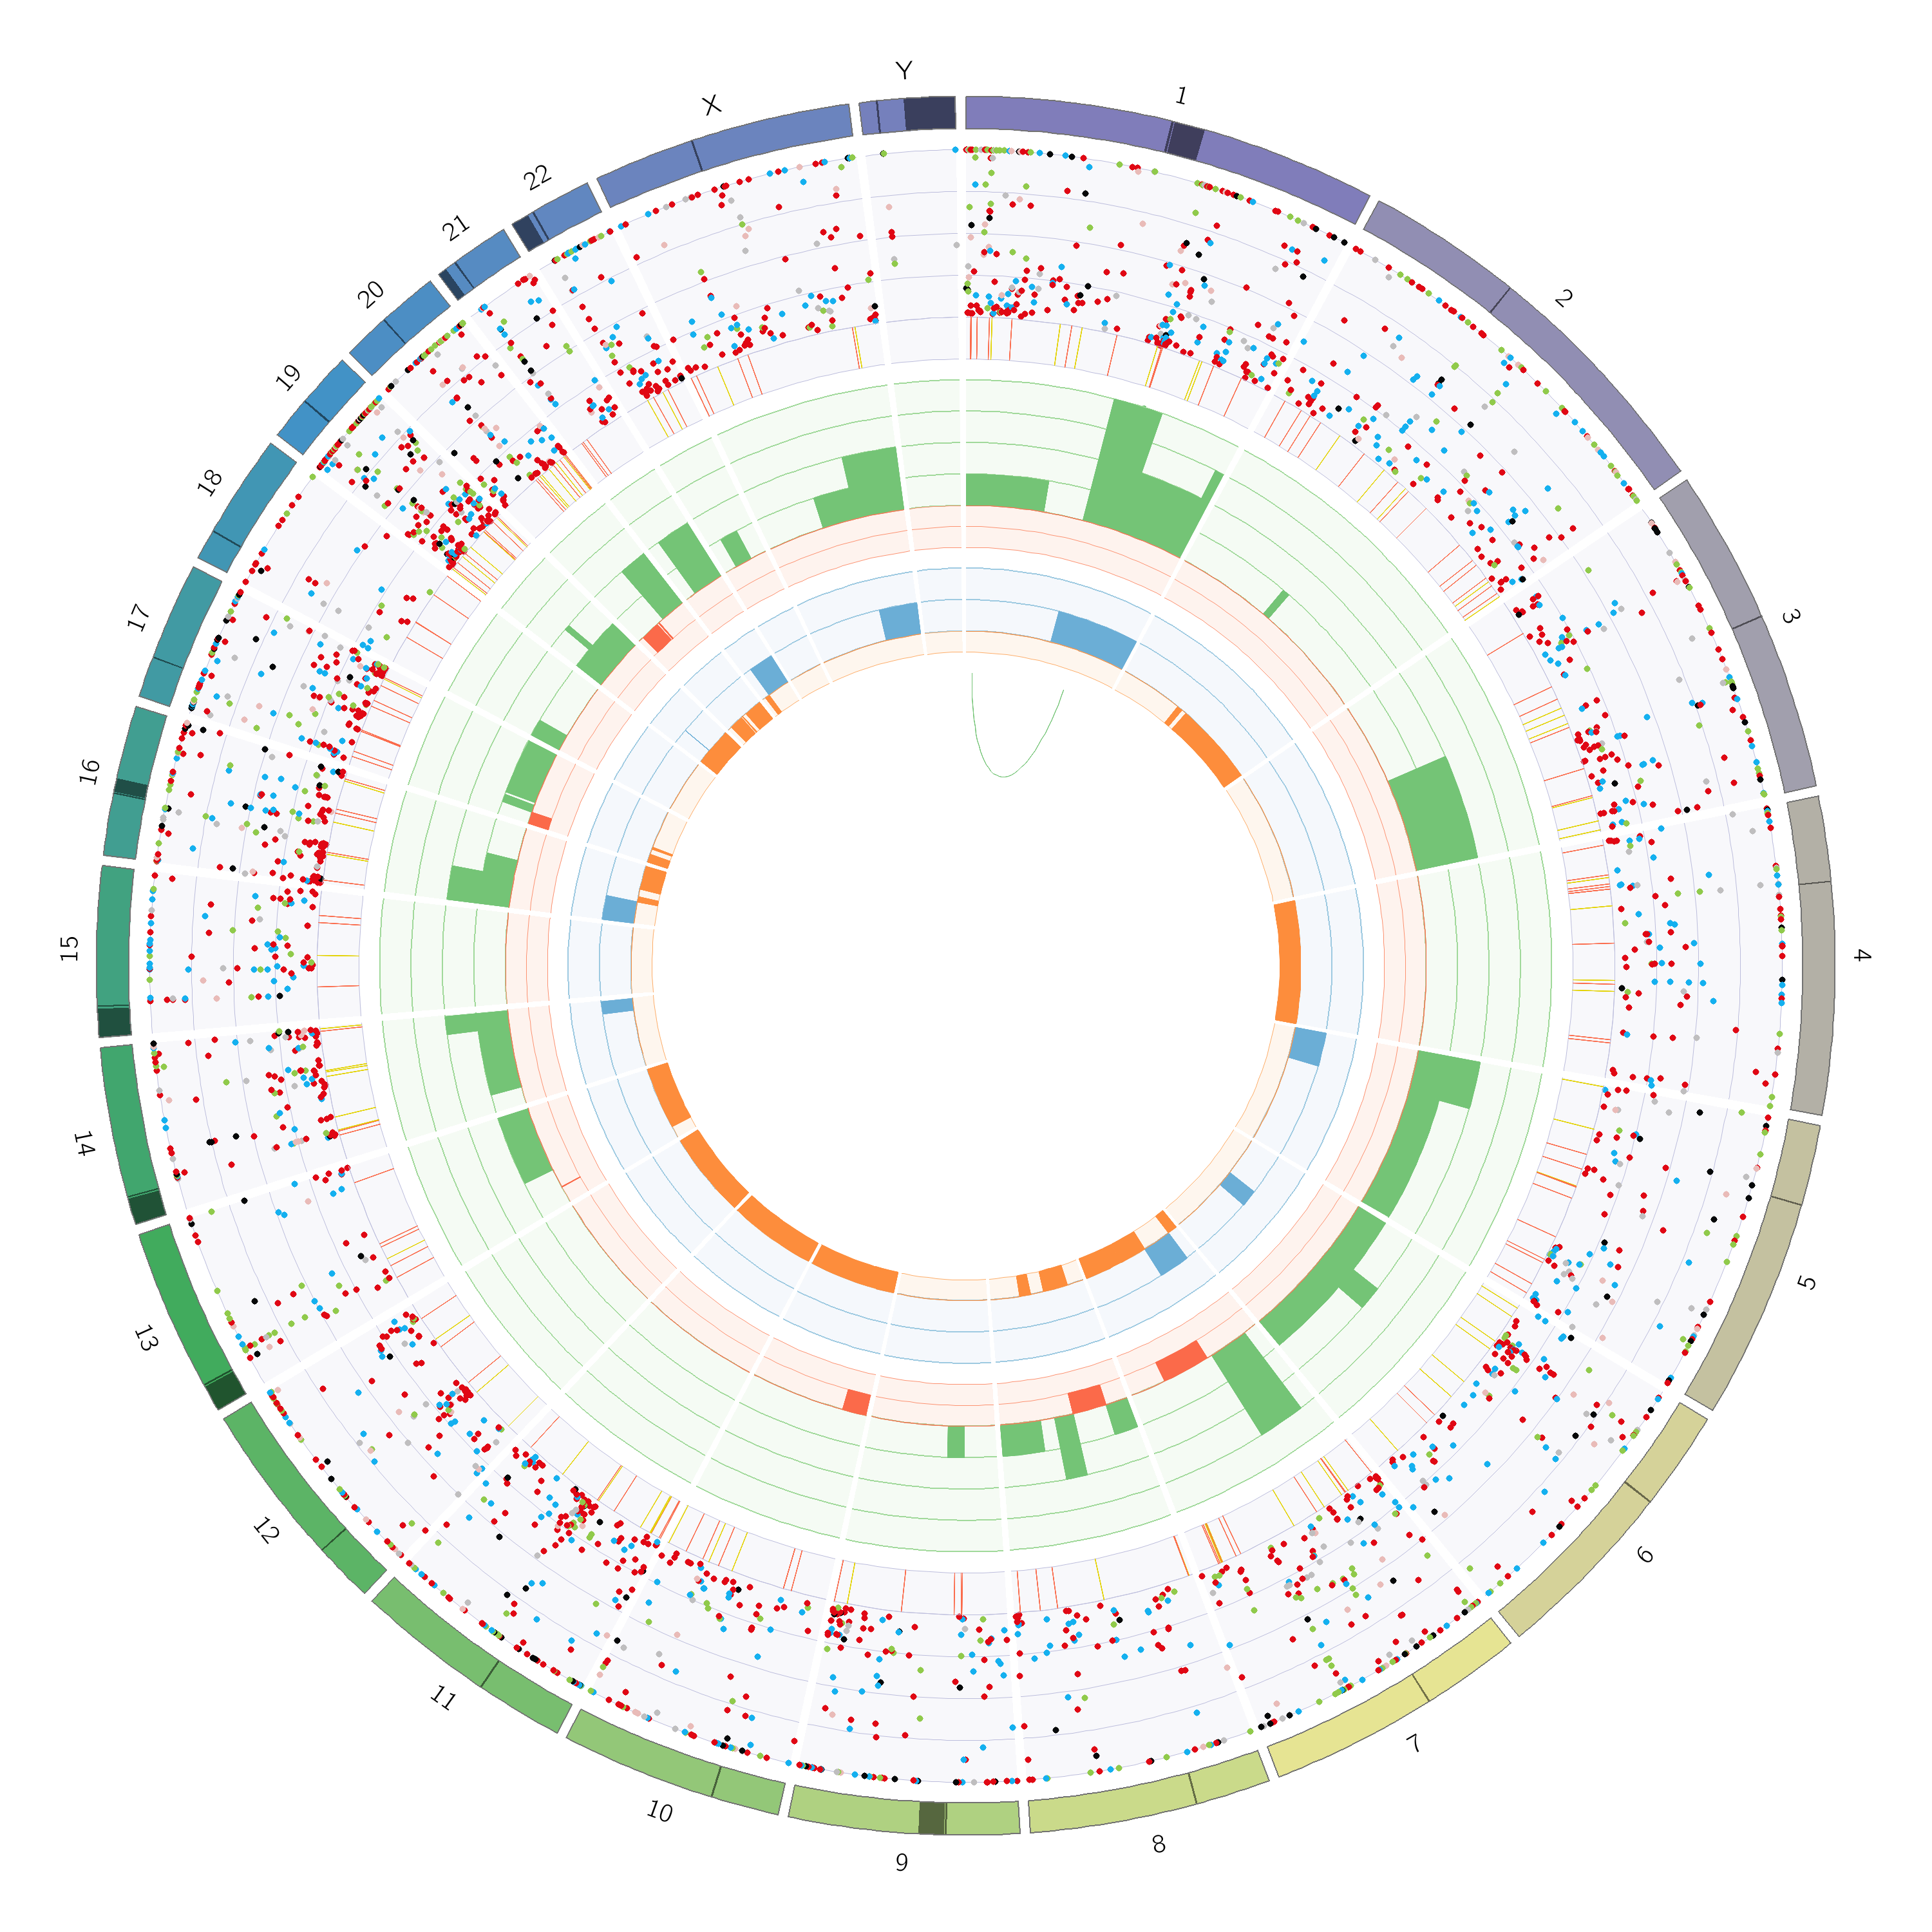
\includegraphics[width=.99\linewidth]{Figures/CASCADE/CA51/CA51-566.circos.png}
\caption[Circos plot of patient CA-I sample 566]{Circos plot of patient CA-I sample 566 with somatic structural variants with allele frequency $> 0.2$: outer first ring shows the canonical chromosomes with gaps (centromere, heterochromatin,...) highlighted as darker areas; second ring visualises all somatic SNVs corrected for tumour purity and scaled from 0 to 1, the colour representing the base change of SNV like in \protect\textcite{Alexandrov2013}; vertical lines directly under the SNVs symbolise InDels, with yellow for insertions and red for deletions; the third ring shows the total copy number alterations, with green showing a copy number gain and red a loss, dots at the outer border show a copy number greater than four; the last ring shows the minor copy number, with blue depicting a gain and orange a loss, this ring allows the detection of copy number neutral changes, like loss of heterozygosity; the center shows all structural variants: translocations in blue, deletions in red, insertions in yellow, tandem duplications in green and inversions in black.} \label{fig:ca51.566circos}
\end{figure}

\begin{figure}[ht]
\centering
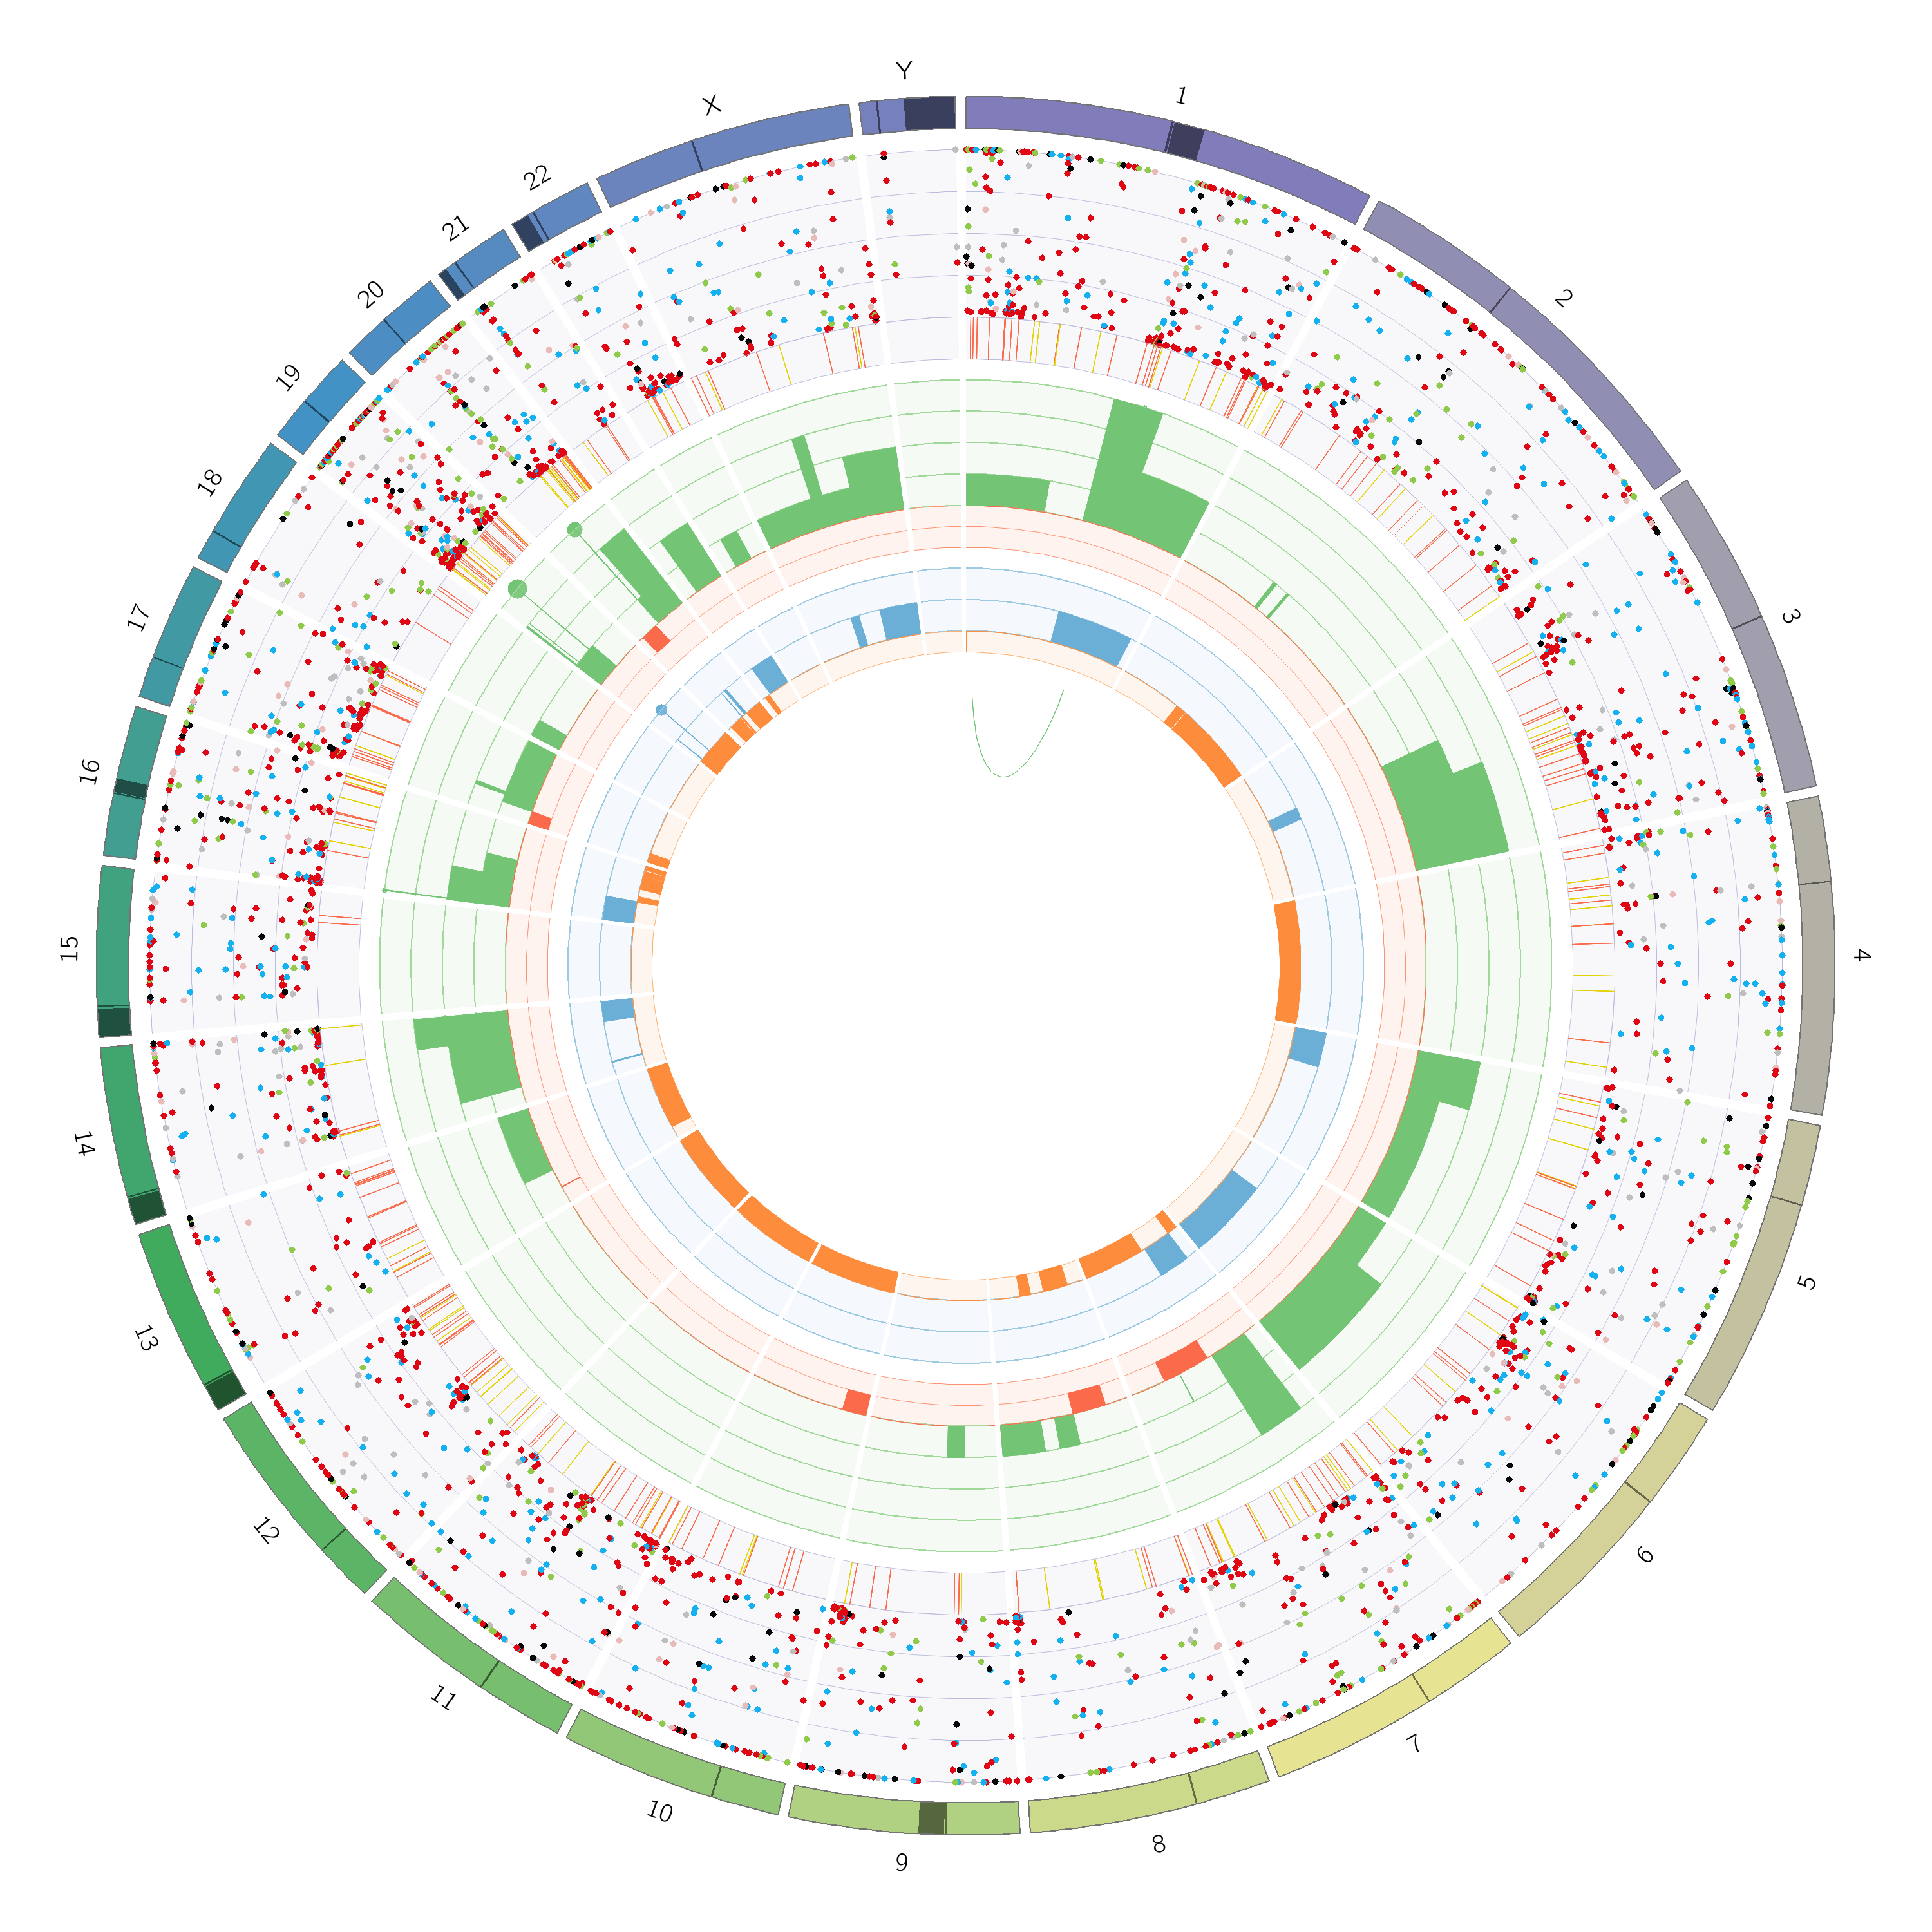
\includegraphics[width=.99\linewidth]{Figures/CASCADE/CA51/CA51-573.circos.png}
\caption[Circos plot of patient CA-I sample 573]{Circos plot of patient CA-I sample 573 with somatic structural variants with allele frequency $> 0.2$: outer first ring shows the canonical chromosomes with gaps (centromere, heterochromatin,...) highlighted as darker areas; second ring visualises all somatic SNVs corrected for tumour purity and scaled from 0 to 1, the colour representing the base change of SNV like in \protect\textcite{Alexandrov2013}; vertical lines directly under the SNVs symbolise InDels, with yellow for insertions and red for deletions; the third ring shows the total copy number alterations, with green showing a copy number gain and red a loss, dots at the outer border show a copy number greater than four; the last ring shows the minor copy number, with blue depicting a gain and orange a loss, this ring allows the detection of copy number neutral changes, like loss of heterozygosity; the center shows all structural variants: translocations in blue, deletions in red, insertions in yellow, tandem duplications in green and inversions in black.} \label{fig:ca51.573circos}
\end{figure}

\begin{figure}[ht]
\centering
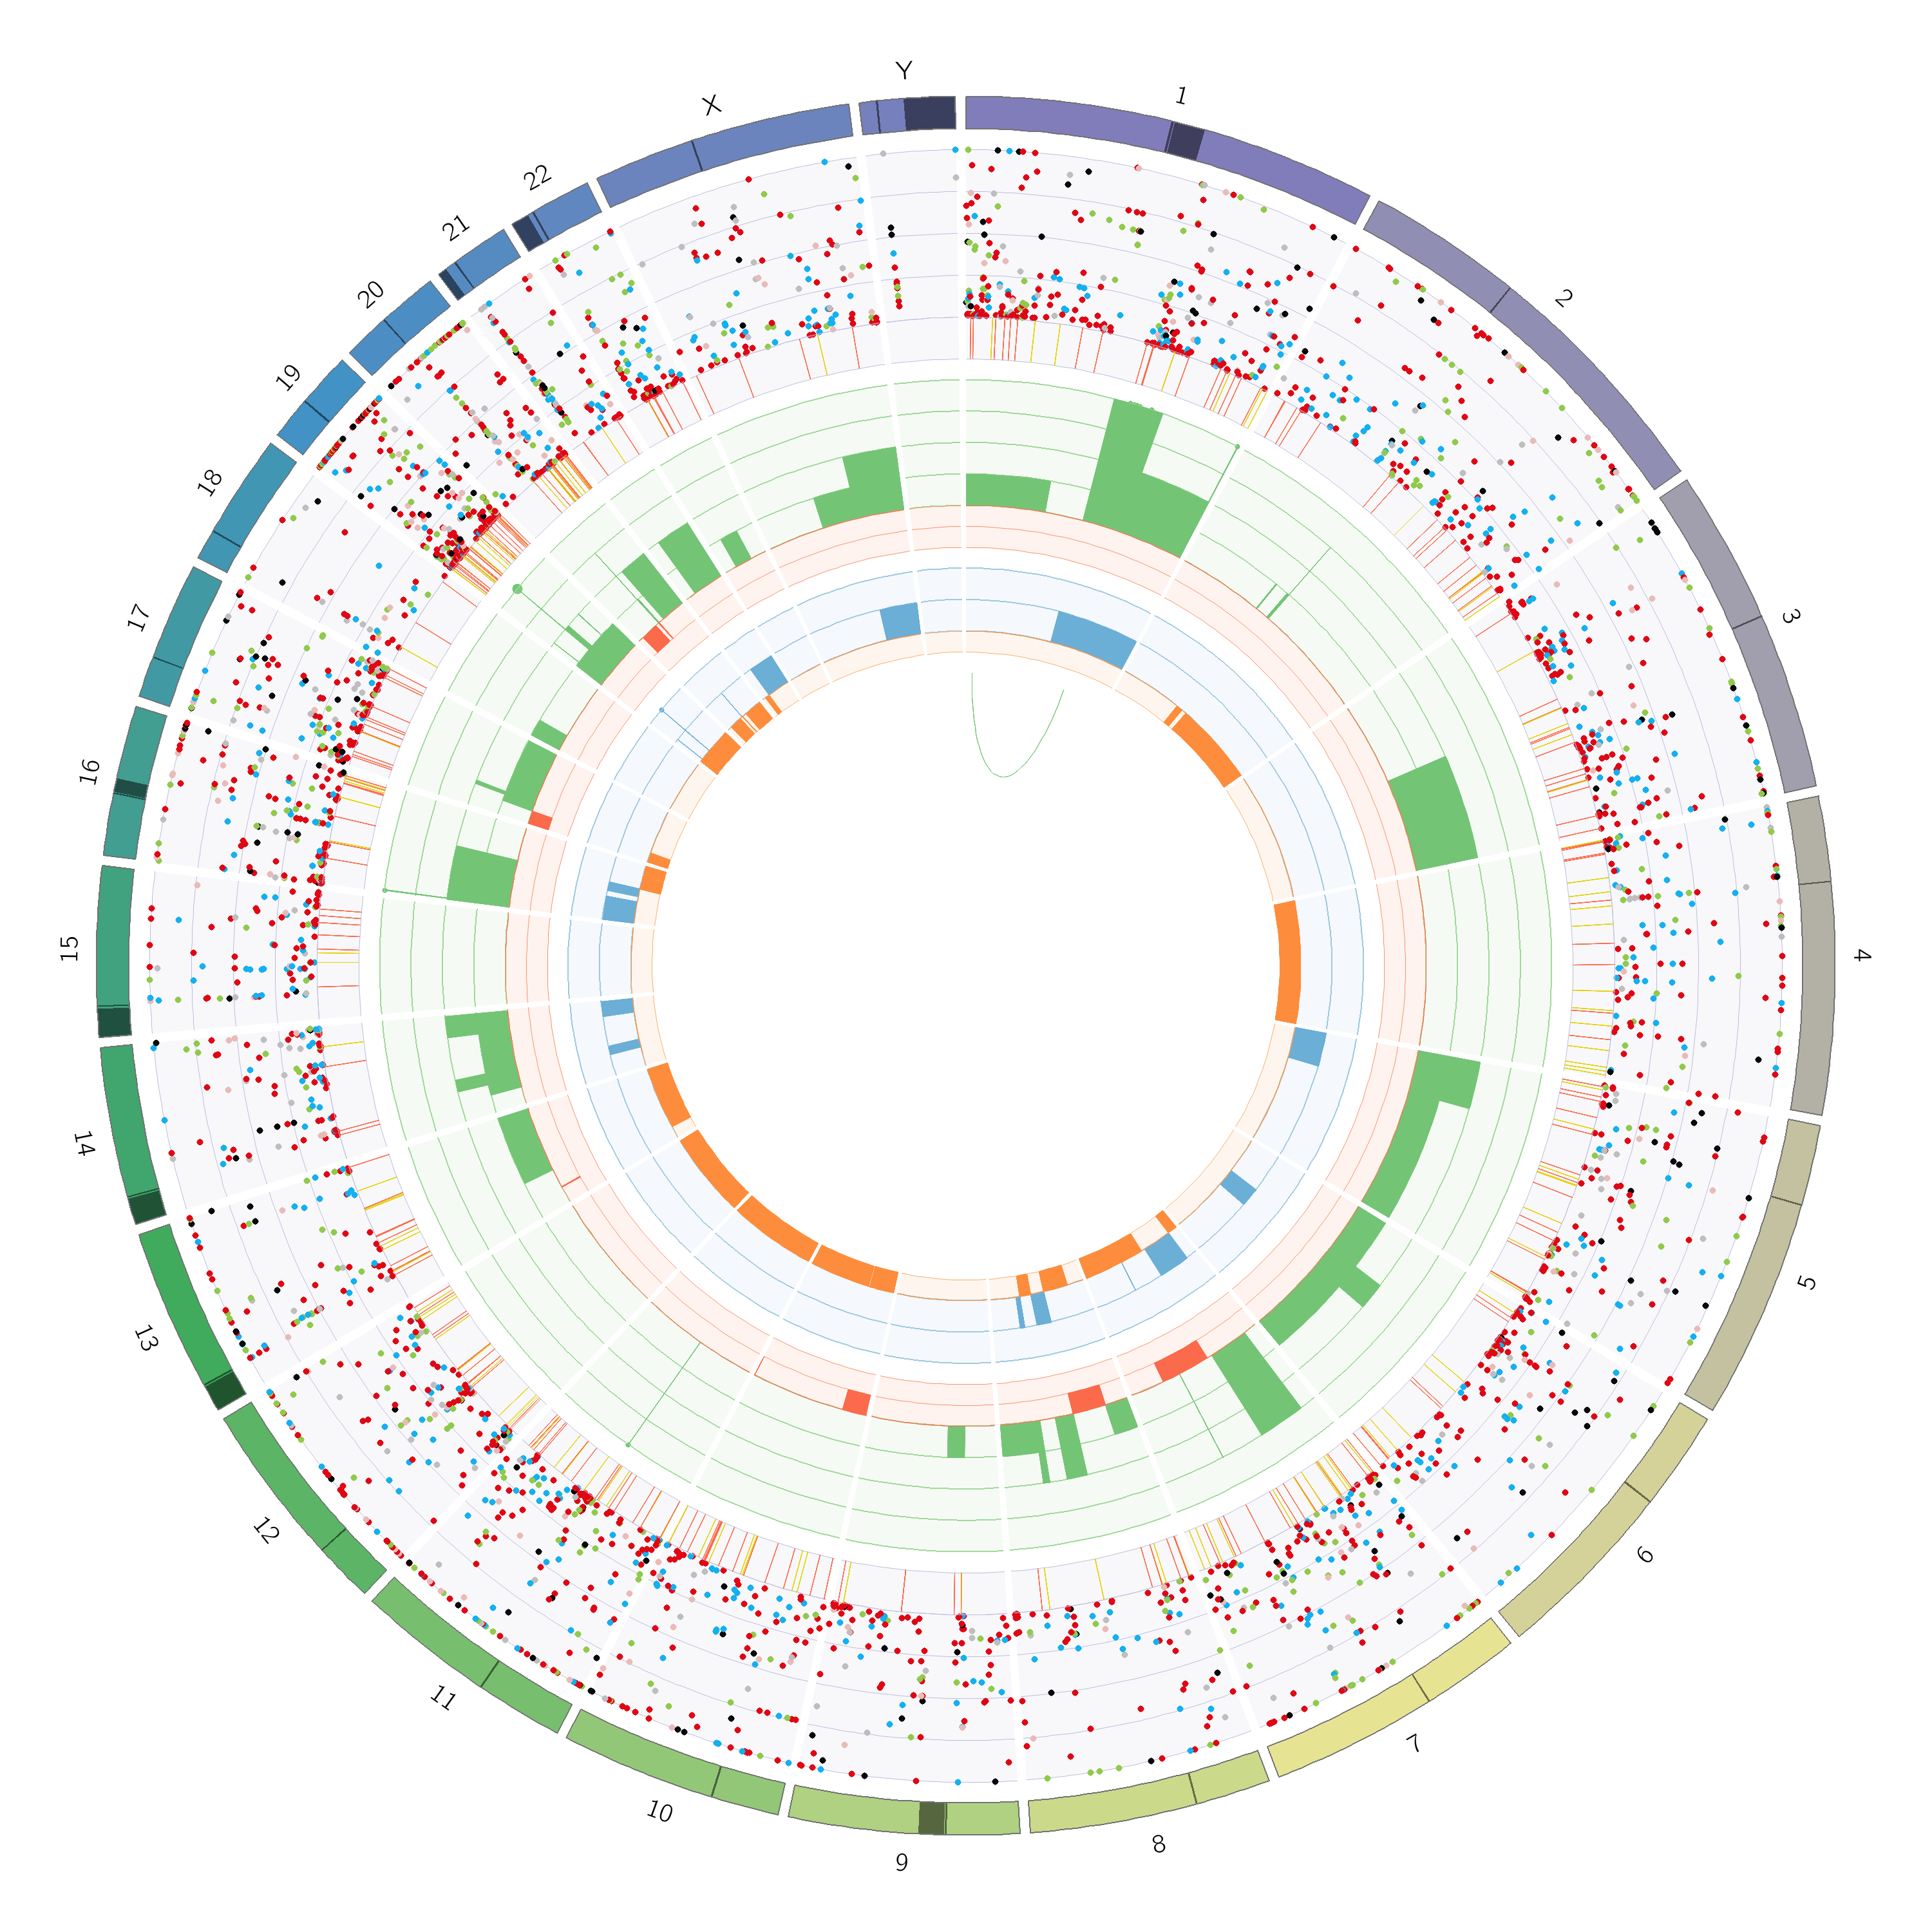
\includegraphics[width=.99\linewidth]{Figures/CASCADE/CA51/CA51-579.circos.png}
\caption[Circos plot of patient CA-I sample 579]{Circos plot of patient CA-I sample 579 with somatic structural variants with allele frequency $> 0.2$: outer first ring shows the canonical chromosomes with gaps (centromere, heterochromatin,...) highlighted as darker areas; second ring visualises all somatic SNVs corrected for tumour purity and scaled from 0 to 1, the colour representing the base change of SNV like in \protect\textcite{Alexandrov2013}; vertical lines directly under the SNVs symbolise InDels, with yellow for insertions and red for deletions; the third ring shows the total copy number alterations, with green showing a copy number gain and red a loss, dots at the outer border show a copy number greater than four; the last ring shows the minor copy number, with blue depicting a gain and orange a loss, this ring allows the detection of copy number neutral changes, like loss of heterozygosity; the center shows all structural variants: translocations in blue, deletions in red, insertions in yellow, tandem duplications in green and inversions in black.} \label{fig:ca51.579circos}
\end{figure}

\begin{figure}[ht]
\centering
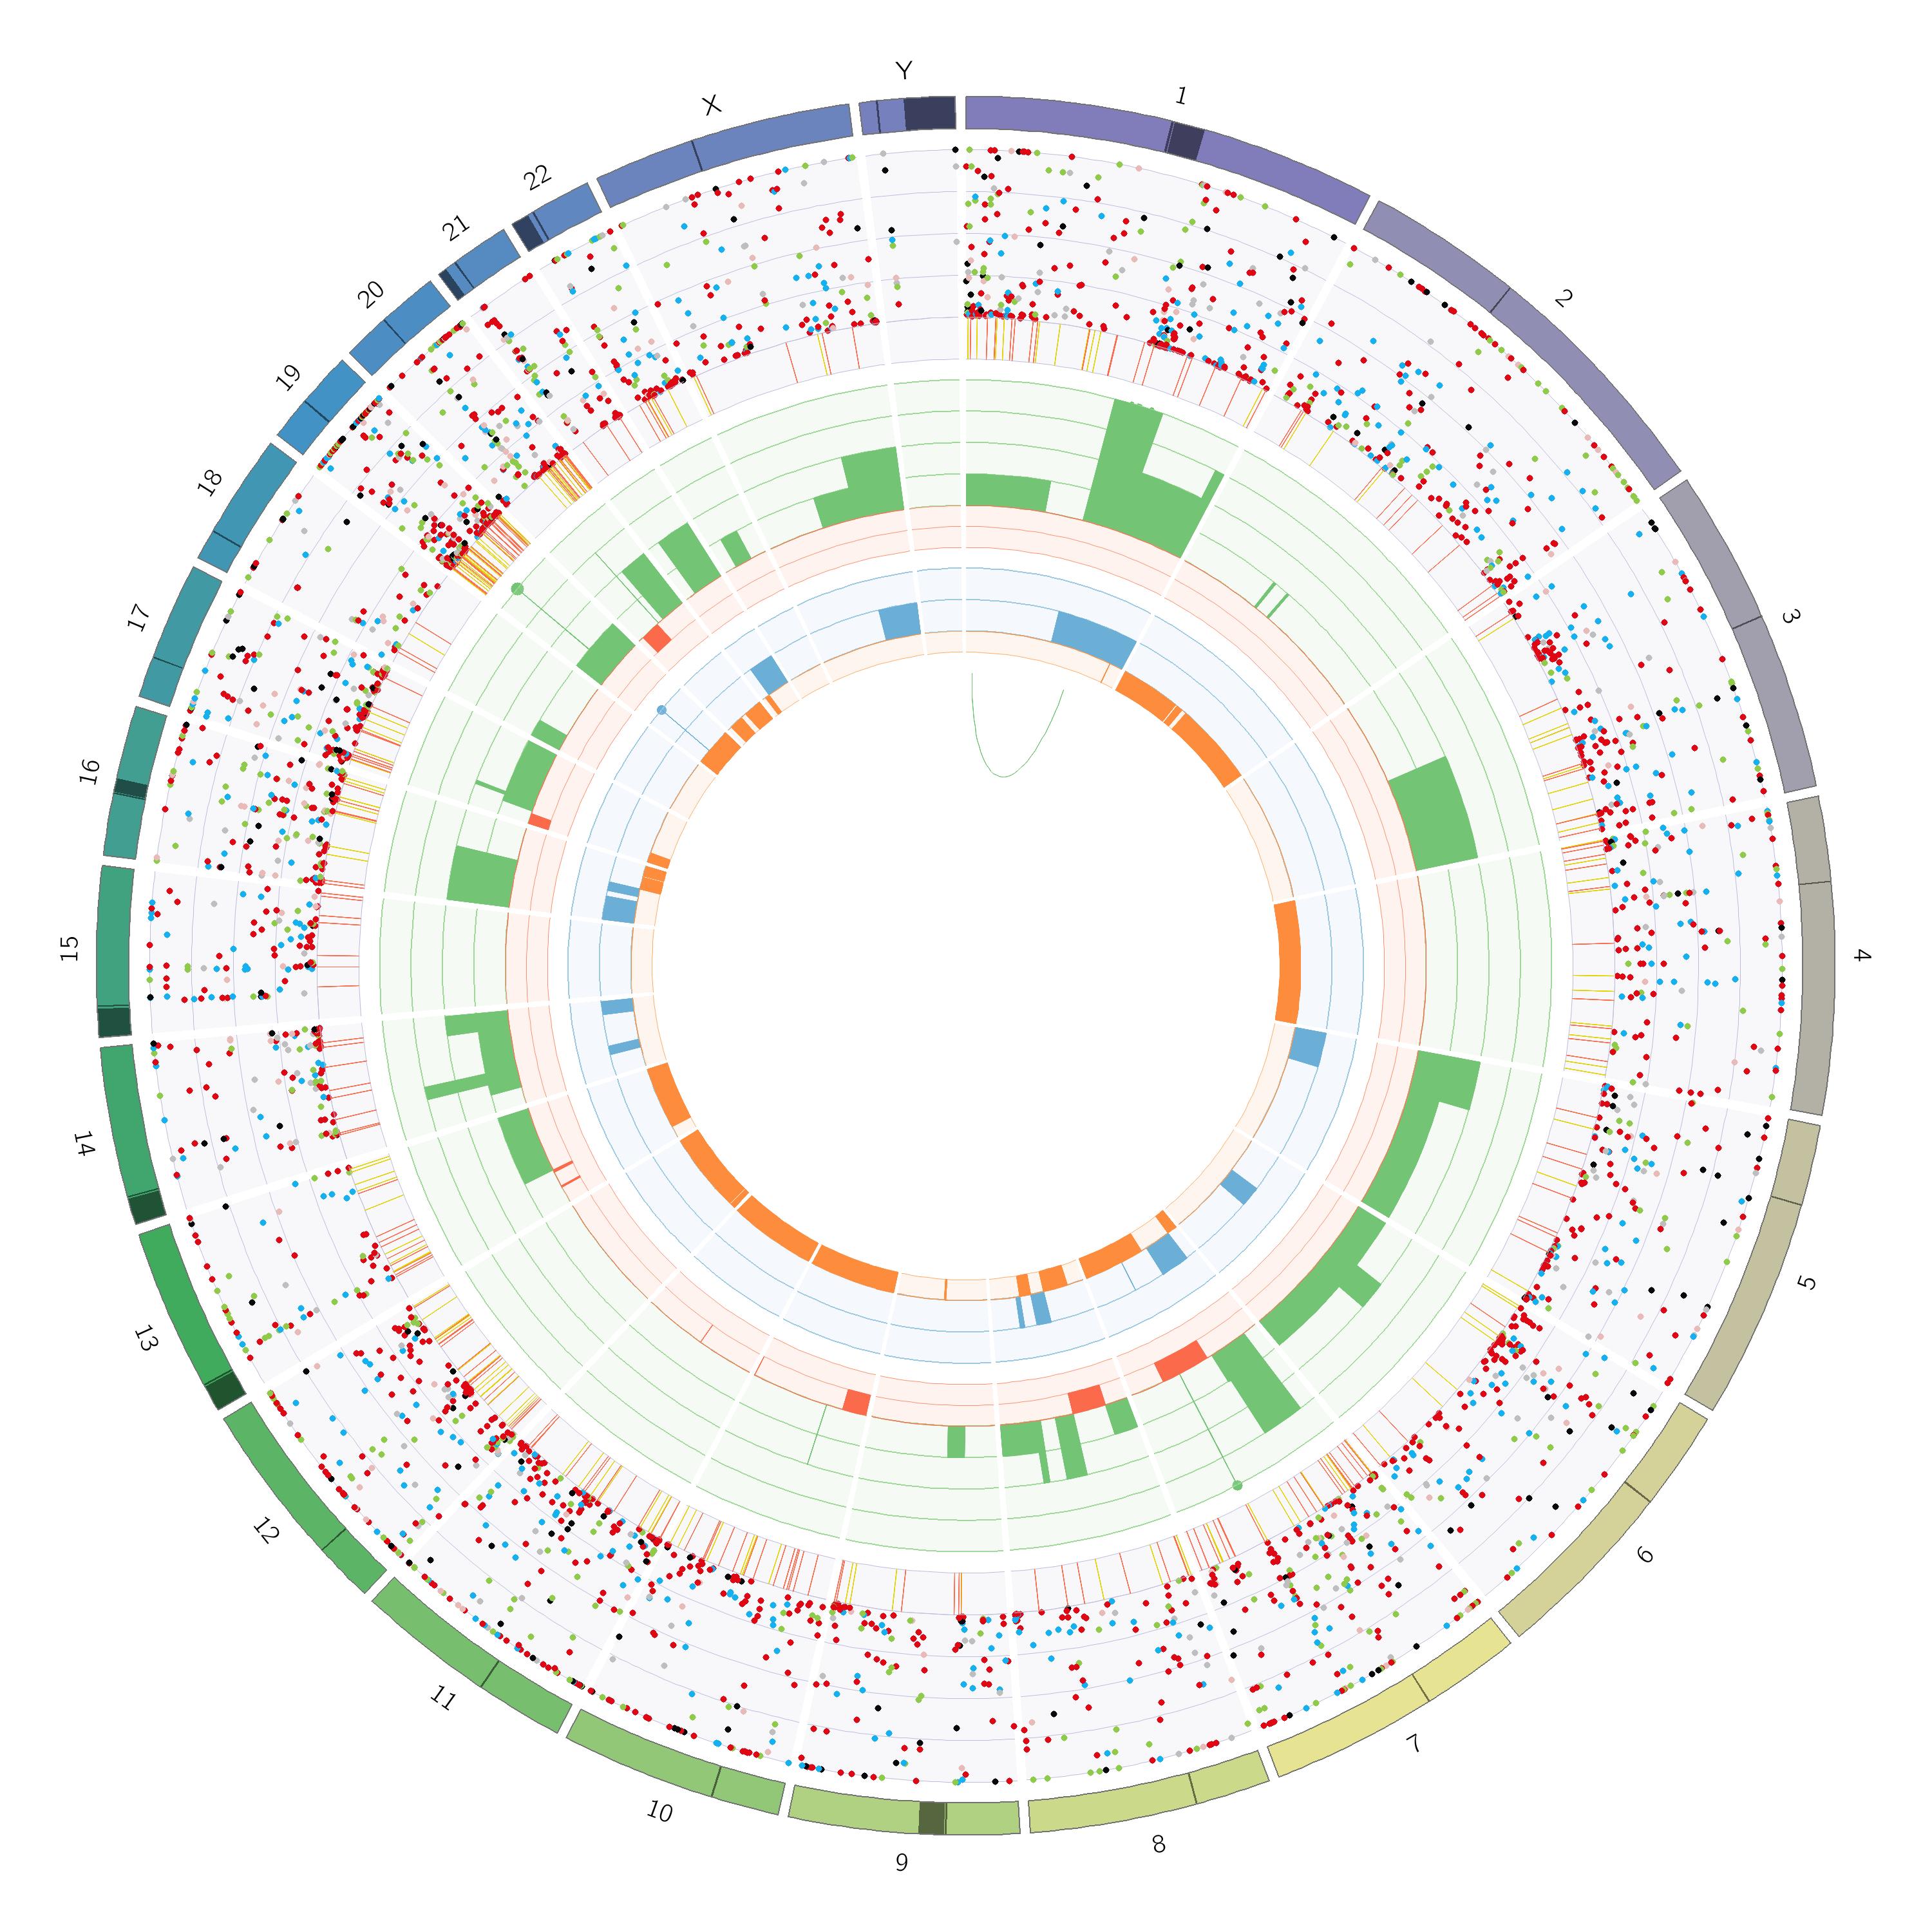
\includegraphics[width=.99\linewidth]{Figures/CASCADE/CA51/CA51-583.circos.png}
\caption[Circos plot of patient CA-I sample 583]{Circos plot of patient CA-I sample 583 with somatic structural variants with allele frequency $> 0.2$: outer first ring shows the canonical chromosomes with gaps (centromere, heterochromatin,...) highlighted as darker areas; second ring visualises all somatic SNVs corrected for tumour purity and scaled from 0 to 1, the colour representing the base change of SNV like in \protect\textcite{Alexandrov2013}; vertical lines directly under the SNVs symbolise InDels, with yellow for insertions and red for deletions; the third ring shows the total copy number alterations, with green showing a copy number gain and red a loss, dots at the outer border show a copy number greater than four; the last ring shows the minor copy number, with blue depicting a gain and orange a loss, this ring allows the detection of copy number neutral changes, like loss of heterozygosity; the center shows all structural variants: translocations in blue, deletions in red, insertions in yellow, tandem duplications in green and inversions in black.} \label{fig:ca51.583circos}
\end{figure}


\cleardoublepage
\subsection{Patient CA-J}

\begin{figure}[ht]
\centering
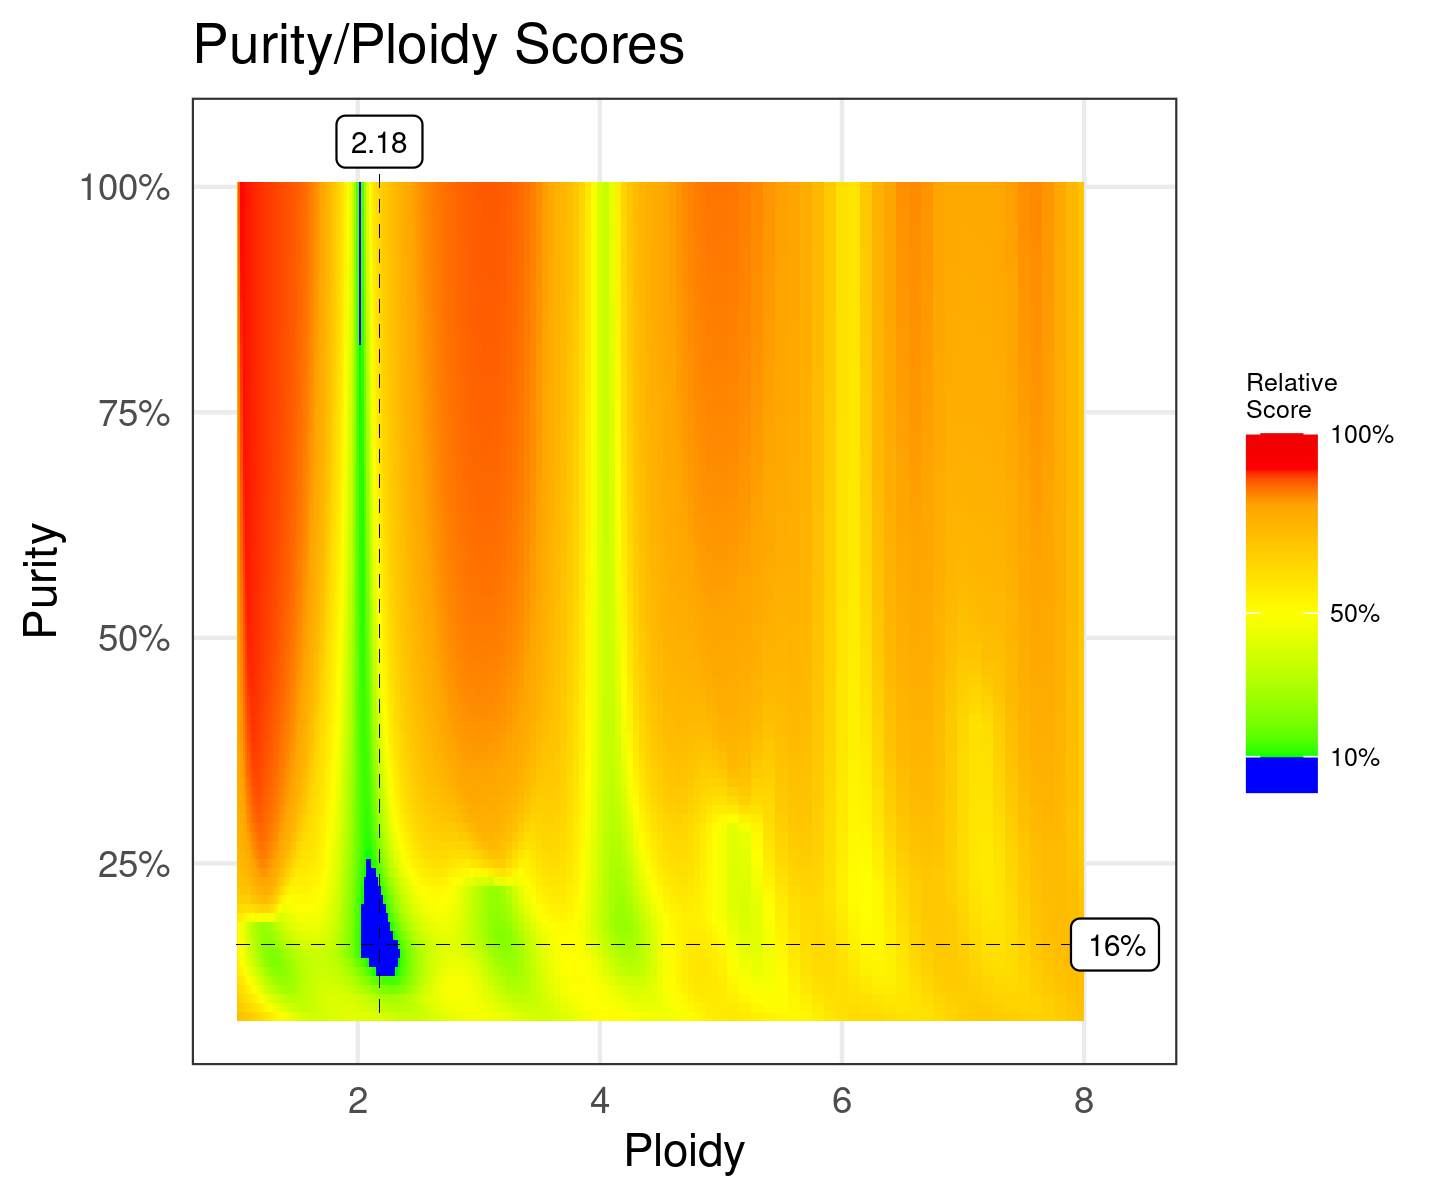
\includegraphics[width=.99\linewidth]{Figures/CASCADE/CA80/CA80-2.purity.range.png}
\caption[Likelihood contours of purity and ploidy solutions of patient CA-J sample 24]{Likelihood contours of purity and ploidy solutions of patient CA-J sample 24: Crosshairs identify the best purity and ploidy solution. Other viable solutions are shown in blue} \label{fig:ca80.2contour}
\end{figure}

\begin{figure}[ht]
\centering
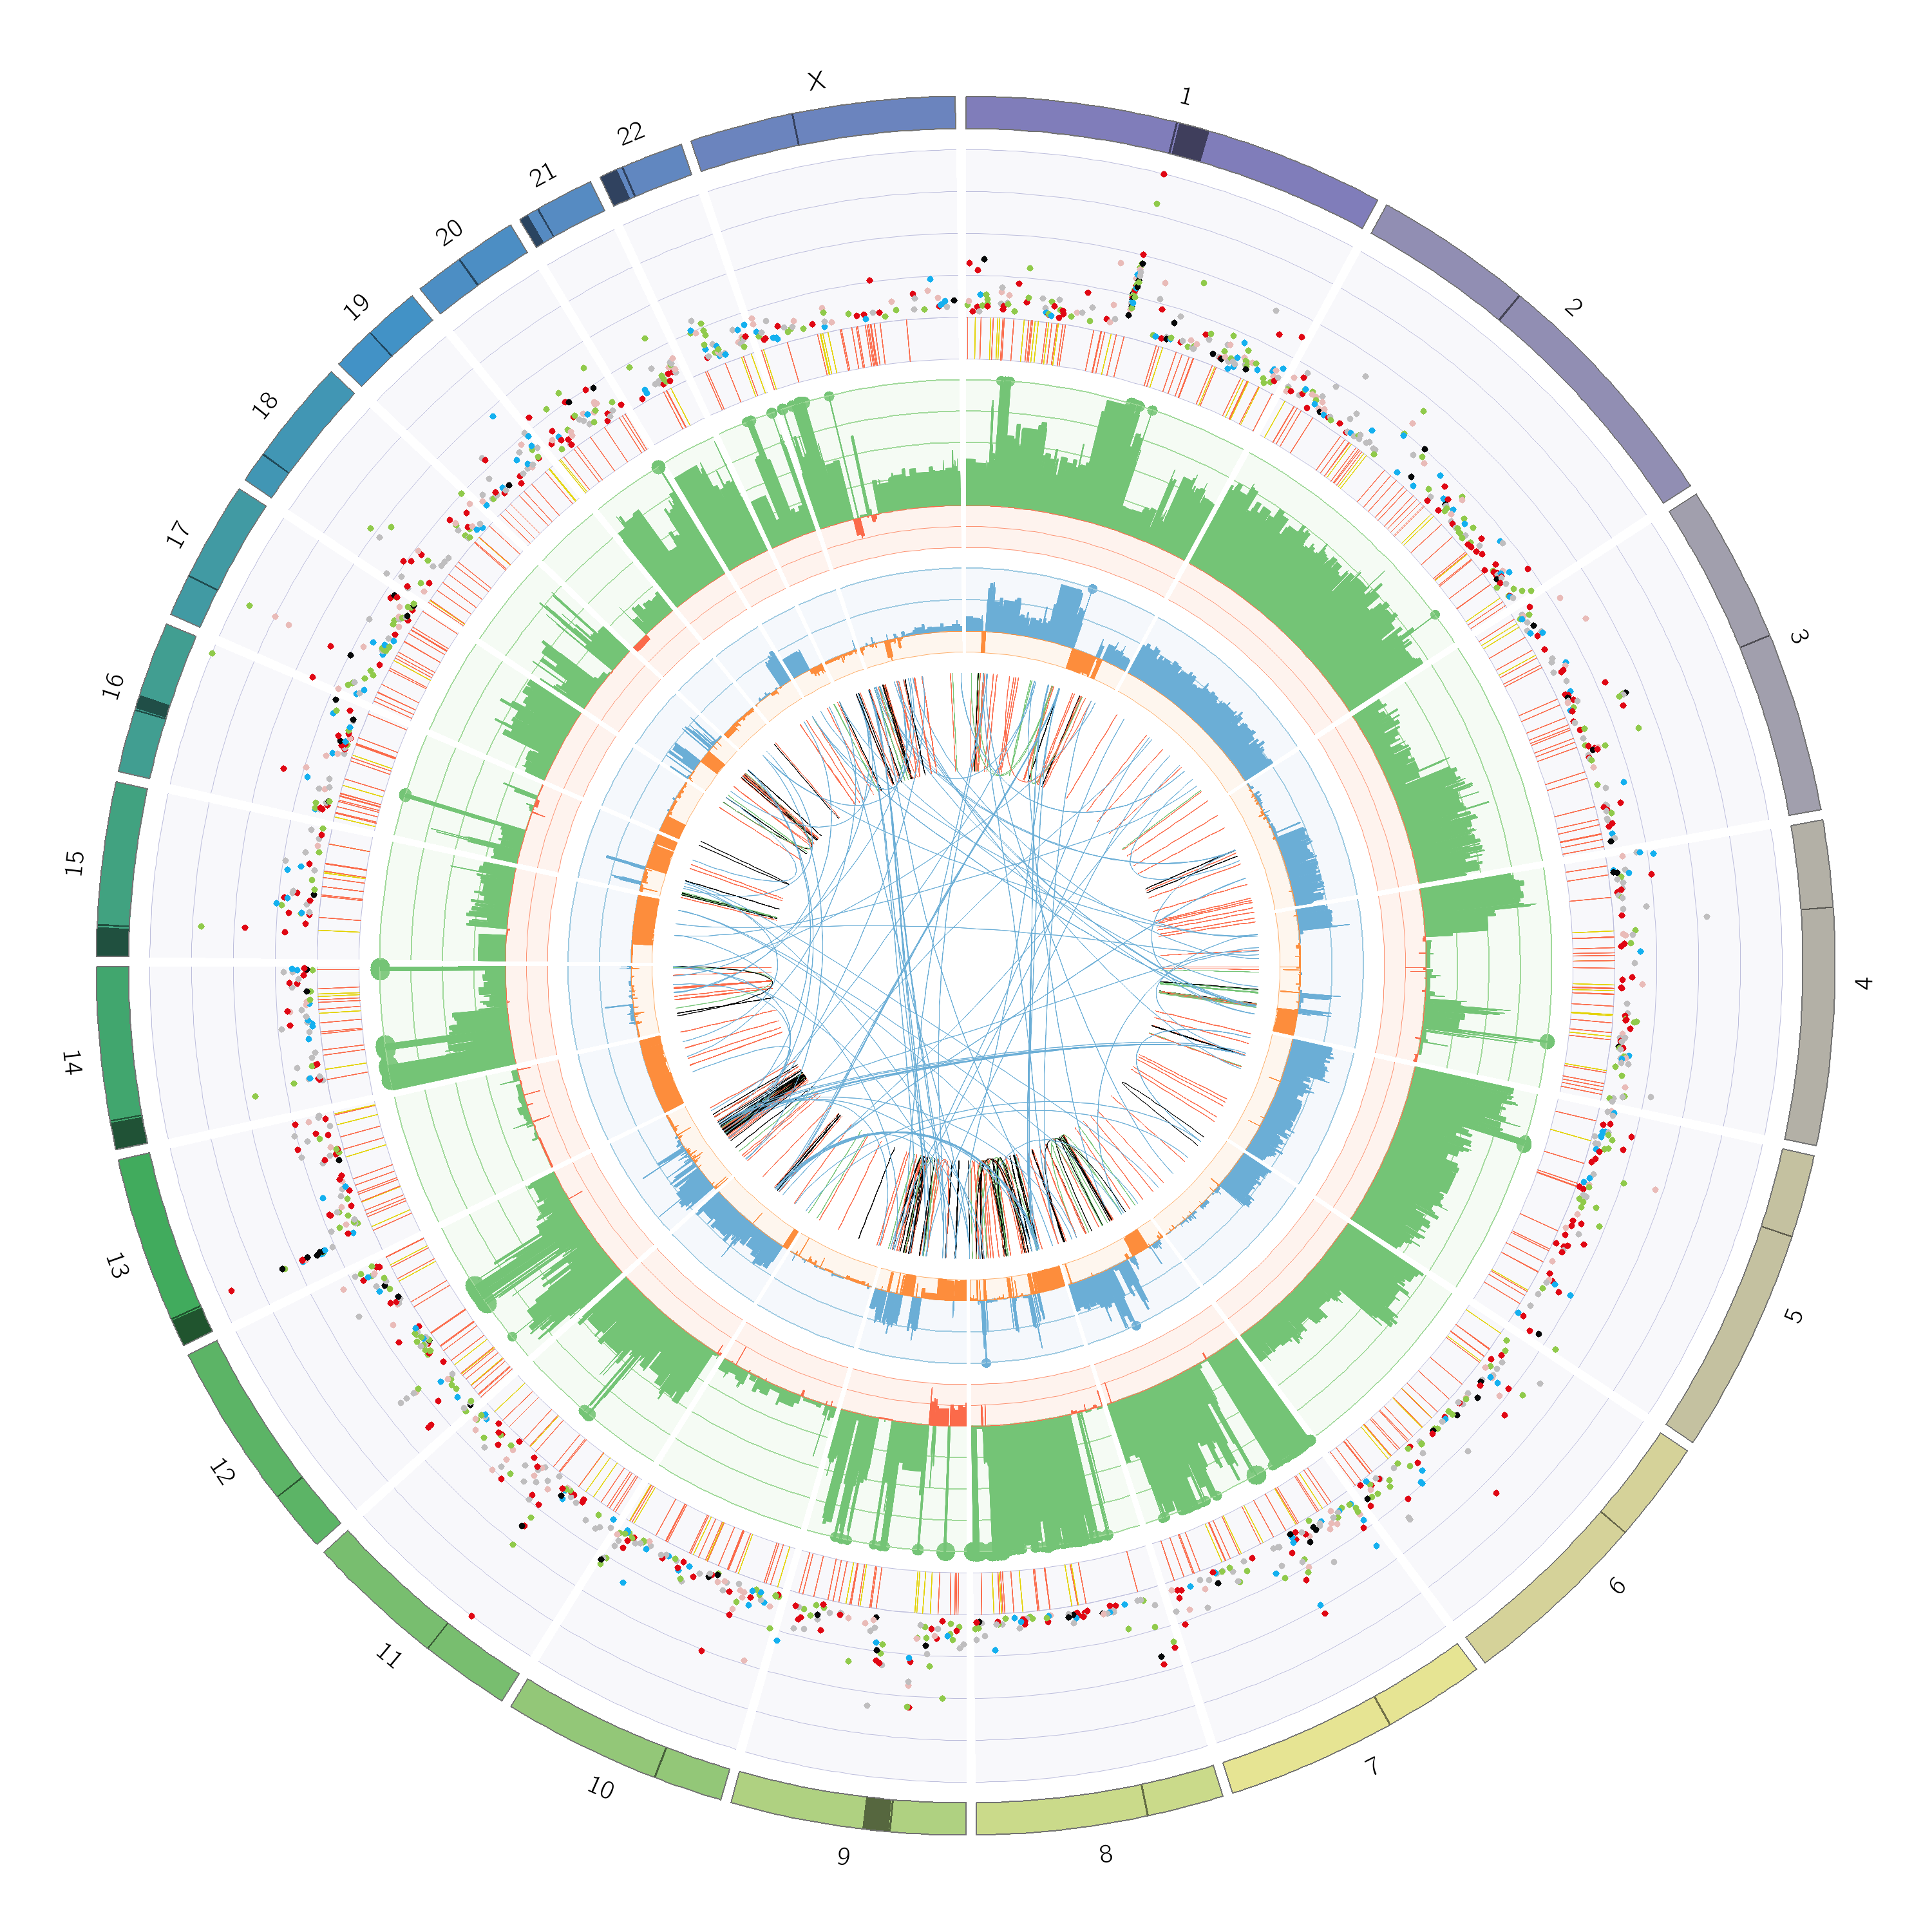
\includegraphics[width=.99\linewidth]{Figures/CASCADE/CA80/CA80-24.circos.png}
\caption[Circos plot of patient CA-J sample 24]{Circos plot of patient CA-J sample 24 with somatic structural variants with allele frequency $\geq 0.10$: outer first ring shows the canonical chromosomes with gaps (centromere, heterochromatin,...) highlighted as darker areas; second ring visualises all somatic SNVs corrected for tumour purity and scaled from 0 to 1, the colour representing the base change of SNV like in \protect\textcite{Alexandrov2013}; vertical lines directly under the SNVs symbolise InDels, with yellow for insertions and red for deletions; the third ring shows the total copy number alterations, with green showing a copy number gain and red a loss, dots at the outer border show a copy number greater than four; the last ring shows the minor copy number, with blue depicting a gain and orange a loss, this ring allows the detection of copy number neutral changes, like loss of heterozygosity; the center shows all structural variants: translocations in blue, deletions in red, insertions in yellow, tandem duplications in green and inversions in black.} \label{fig:ca80.24circos}
\end{figure}

\begin{figure}[ht]
\centering
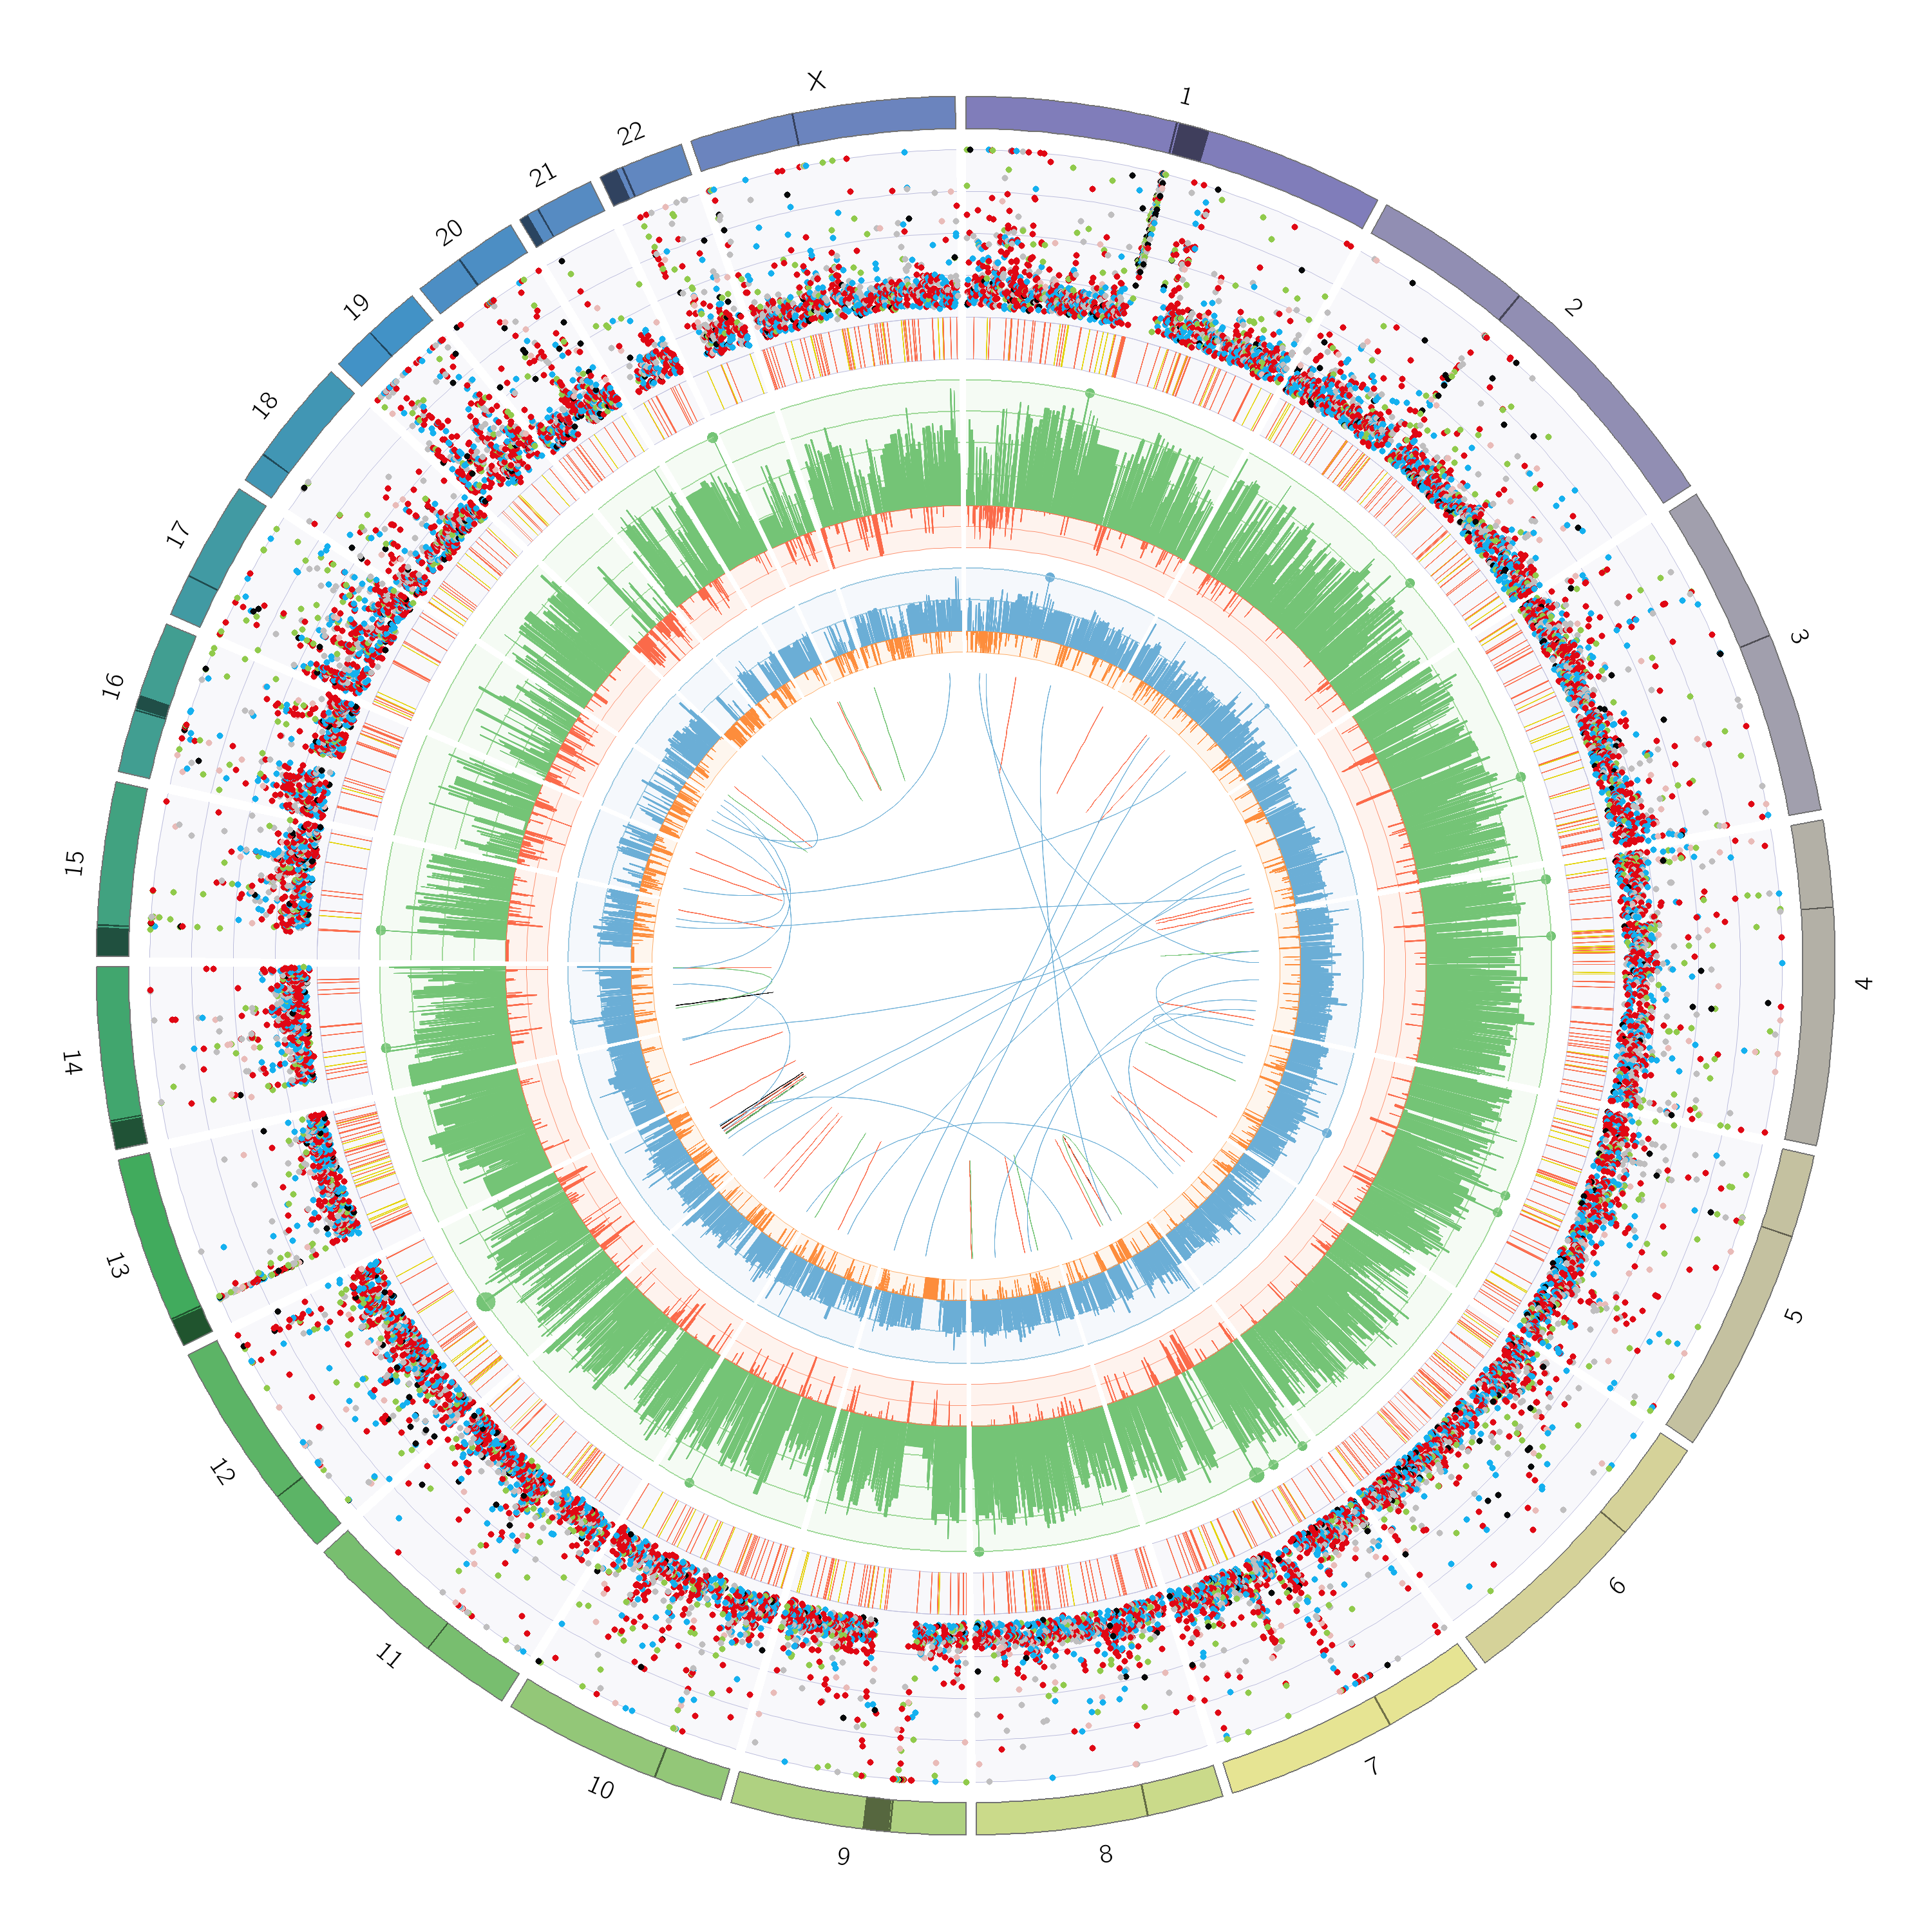
\includegraphics[width=.99\linewidth]{Figures/CASCADE/CA80/CA80-28.circos.png}
\caption[Circos plot of patient CA-J sample 28]{Circos plot of patient CA-J sample 28 with somatic structural variants with allele frequency $\geq 0.10$: outer first ring shows the canonical chromosomes with gaps (centromere, heterochromatin,...) highlighted as darker areas; second ring visualises all somatic SNVs corrected for tumour purity and scaled from 0 to 1, the colour representing the base change of SNV like in \protect\textcite{Alexandrov2013}; vertical lines directly under the SNVs symbolise InDels, with yellow for insertions and red for deletions; the third ring shows the total copy number alterations, with green showing a copy number gain and red a loss, dots at the outer border show a copy number greater than four; the last ring shows the minor copy number, with blue depicting a gain and orange a loss, this ring allows the detection of copy number neutral changes, like loss of heterozygosity; the center shows all structural variants: translocations in blue, deletions in red, insertions in yellow, tandem duplications in green and inversions in black.} \label{fig:ca80.28circos}
\end{figure}

\begin{figure}[ht]
\centering
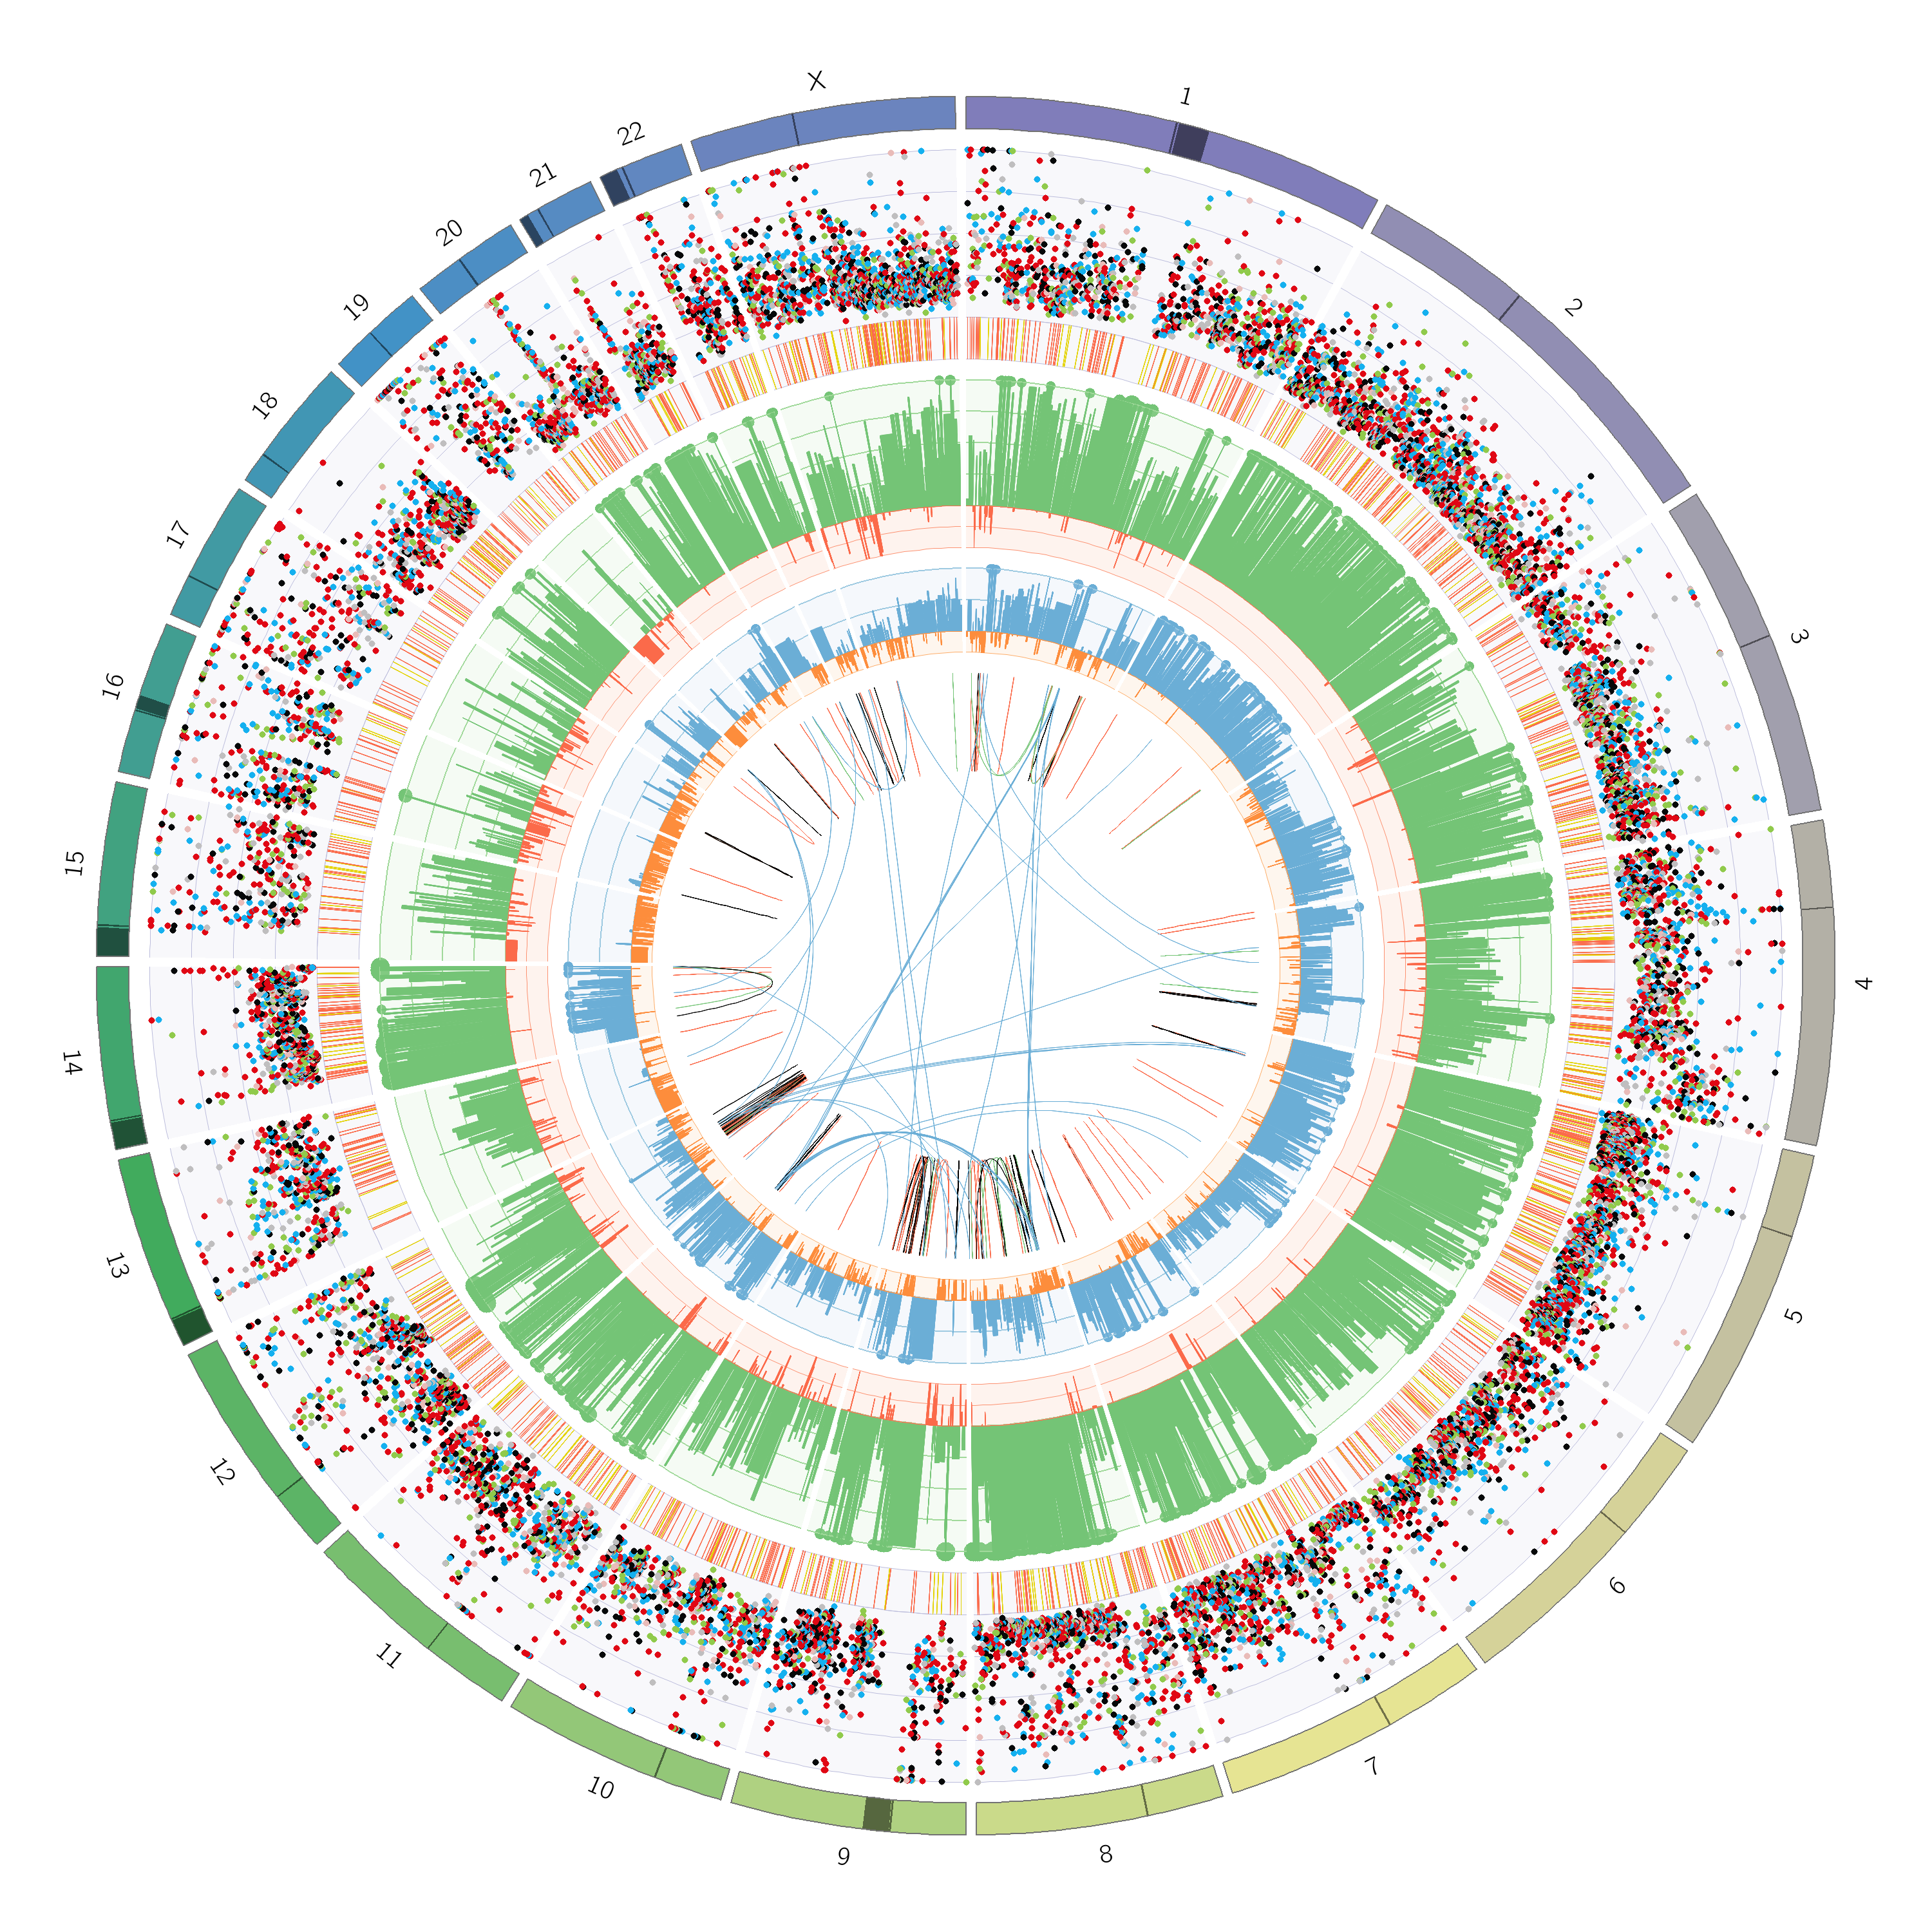
\includegraphics[width=.99\linewidth]{Figures/CASCADE/CA80/CA80-32.circos.png}
\caption[Circos plot of patient CA-J sample 32]{Circos plot of patient CA-J sample 32 with somatic structural variants with allele frequency $\geq 0.10$: outer first ring shows the canonical chromosomes with gaps (centromere, heterochromatin,...) highlighted as darker areas; second ring visualises all somatic SNVs corrected for tumour purity and scaled from 0 to 1, the colour representing the base change of SNV like in \protect\textcite{Alexandrov2013}; vertical lines directly under the SNVs symbolise InDels, with yellow for insertions and red for deletions; the third ring shows the total copy number alterations, with green showing a copy number gain and red a loss, dots at the outer border show a copy number greater than four; the last ring shows the minor copy number, with blue depicting a gain and orange a loss, this ring allows the detection of copy number neutral changes, like loss of heterozygosity; the center shows all structural variants: translocations in blue, deletions in red, insertions in yellow, tandem duplications in green and inversions in black.} \label{fig:ca80.32circos}
\end{figure}

\begin{figure}[ht]
\centering
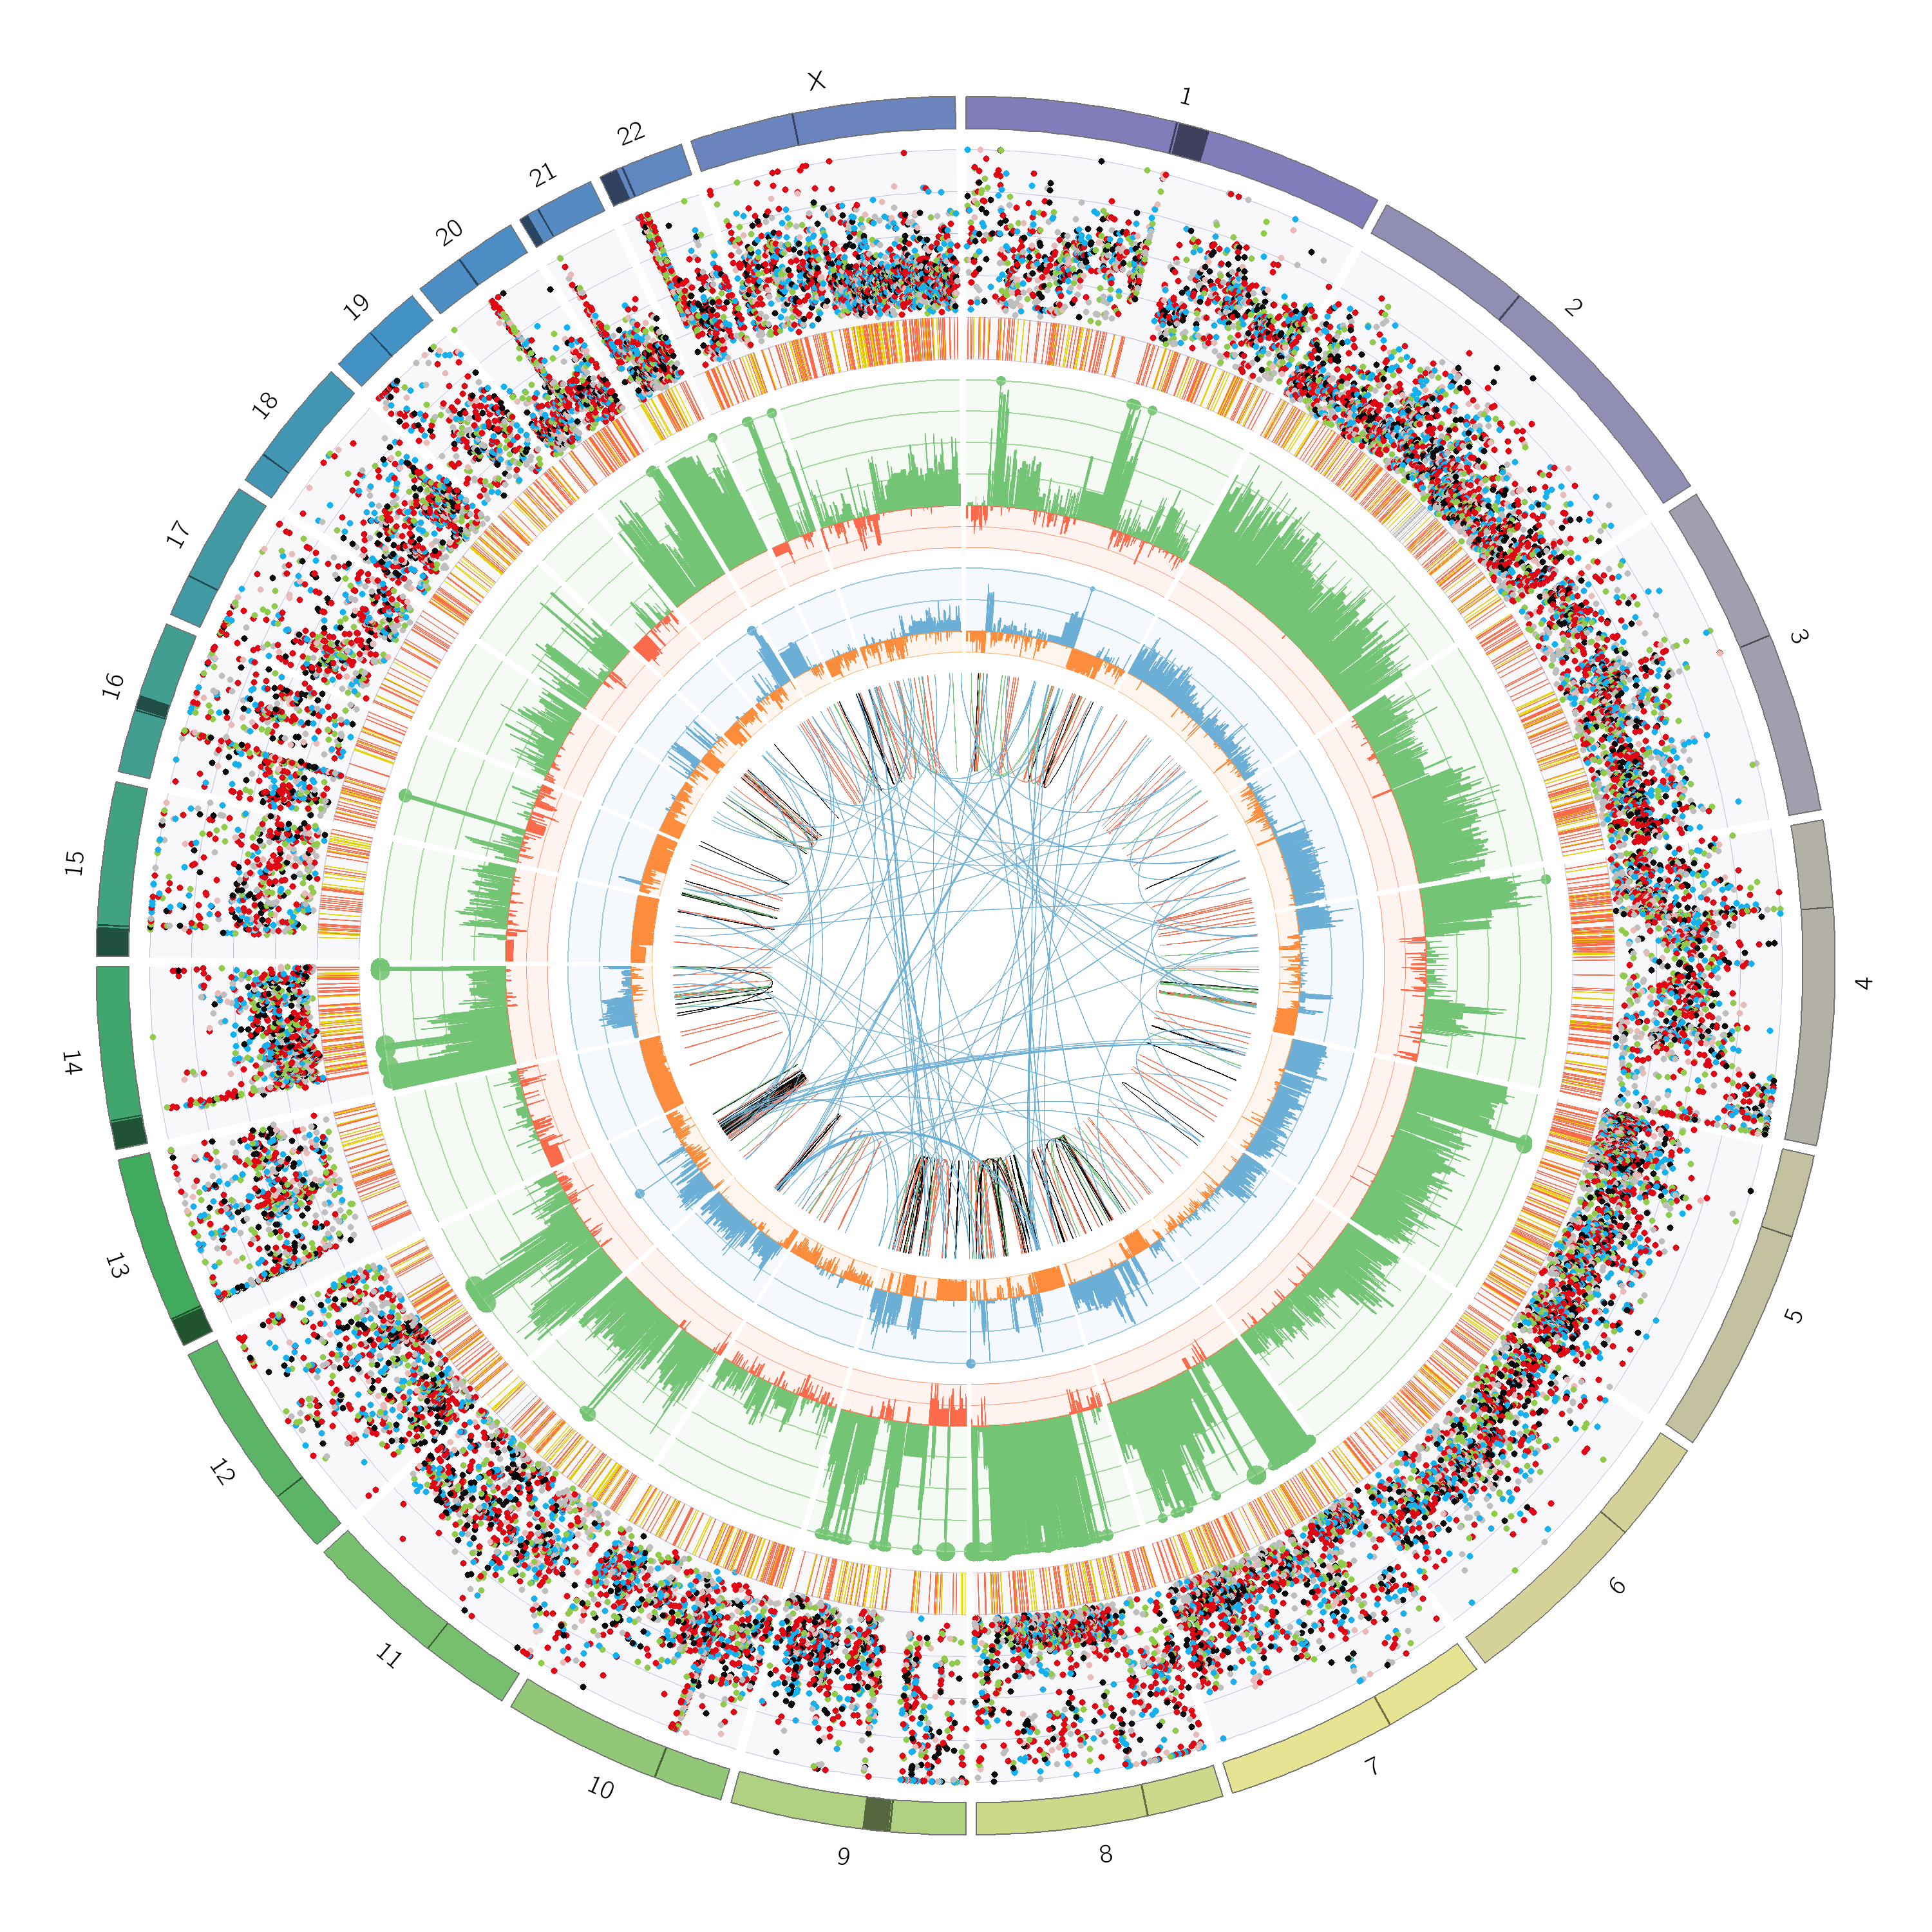
\includegraphics[width=.99\linewidth]{Figures/CASCADE/CA80/CA80-42.circos.png}
\caption[Circos plot of patient CA-J sample 42]{Circos plot of patient CA-J sample 42 with somatic structural variants with allele frequency $\geq 0.10$: outer first ring shows the canonical chromosomes with gaps (centromere, heterochromatin,...) highlighted as darker areas; second ring visualises all somatic SNVs corrected for tumour purity and scaled from 0 to 1, the colour representing the base change of SNV like in \protect\textcite{Alexandrov2013}; vertical lines directly under the SNVs symbolise InDels, with yellow for insertions and red for deletions; the third ring shows the total copy number alterations, with green showing a copy number gain and red a loss, dots at the outer border show a copy number greater than four; the last ring shows the minor copy number, with blue depicting a gain and orange a loss, this ring allows the detection of copy number neutral changes, like loss of heterozygosity; the center shows all structural variants: translocations in blue, deletions in red, insertions in yellow, tandem duplications in green and inversions in black.} \label{fig:ca80.42circos}
\end{figure}

\cleardoublepage
\subsection{Patient CA-K}

\begin{figure}[ht]
\centering
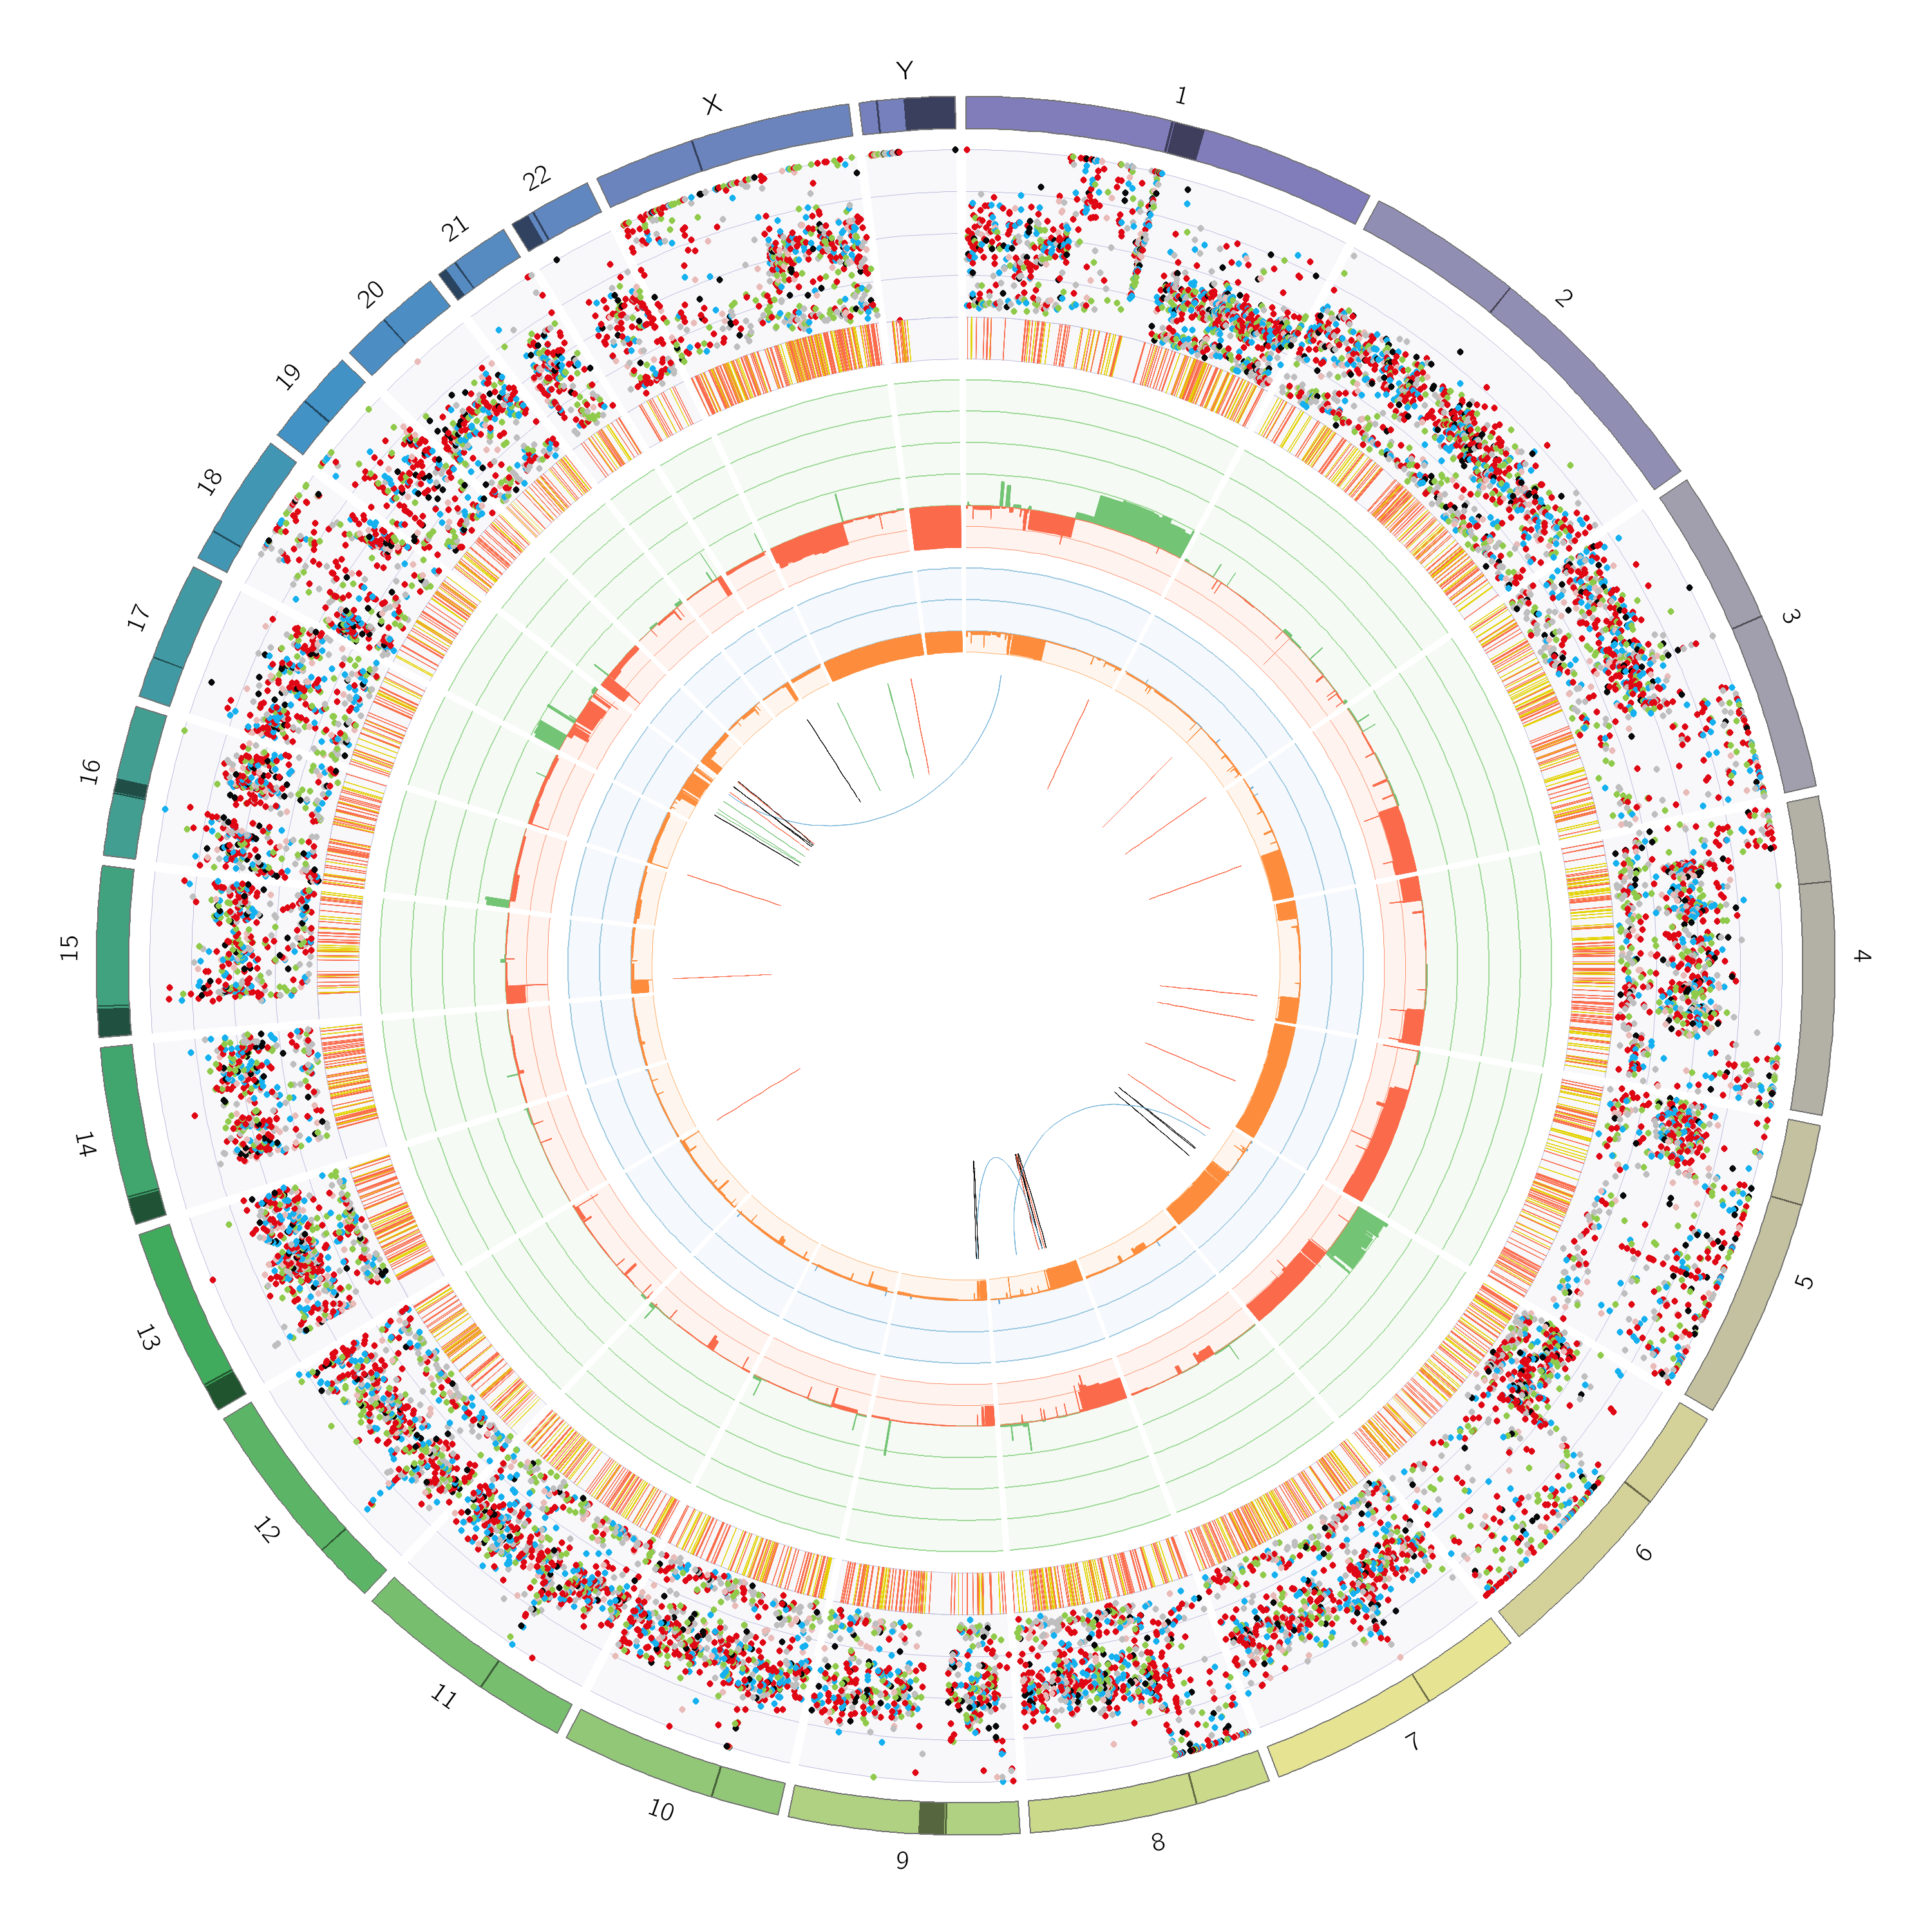
\includegraphics[width=.99\linewidth]{Figures/CASCADE/CA82/CA82-4.circos.png}
\caption[Circos plot of patient CA-K sample 4]{Circos plot of patient CA-K sample 4: outer first ring shows the canonical chromosomes with gaps (centromere, heterochromatin,...) highlighted as darker areas; second ring visualises all somatic SNVs corrected for tumour purity and scaled from 0 to 1, the colour representing the base change of SNV like in \protect\textcite{Alexandrov2013}; vertical lines directly under the SNVs symbolise InDels, with yellow for insertions and red for deletions; the third ring shows the total copy number alterations, with green showing a copy number gain and red a loss, dots at the outer border show a copy number greater than four; the last ring shows the minor copy number, with blue depicting a gain and orange a loss, this ring allows the detection of copy number neutral changes, like loss of heterozygosity; the center shows all structural variants: translocations in blue, deletions in red, insertions in yellow, tandem duplications in green and inversions in black.} \label{fig:ca82.4circos}
\end{figure}

\begin{figure}[ht]
\centering
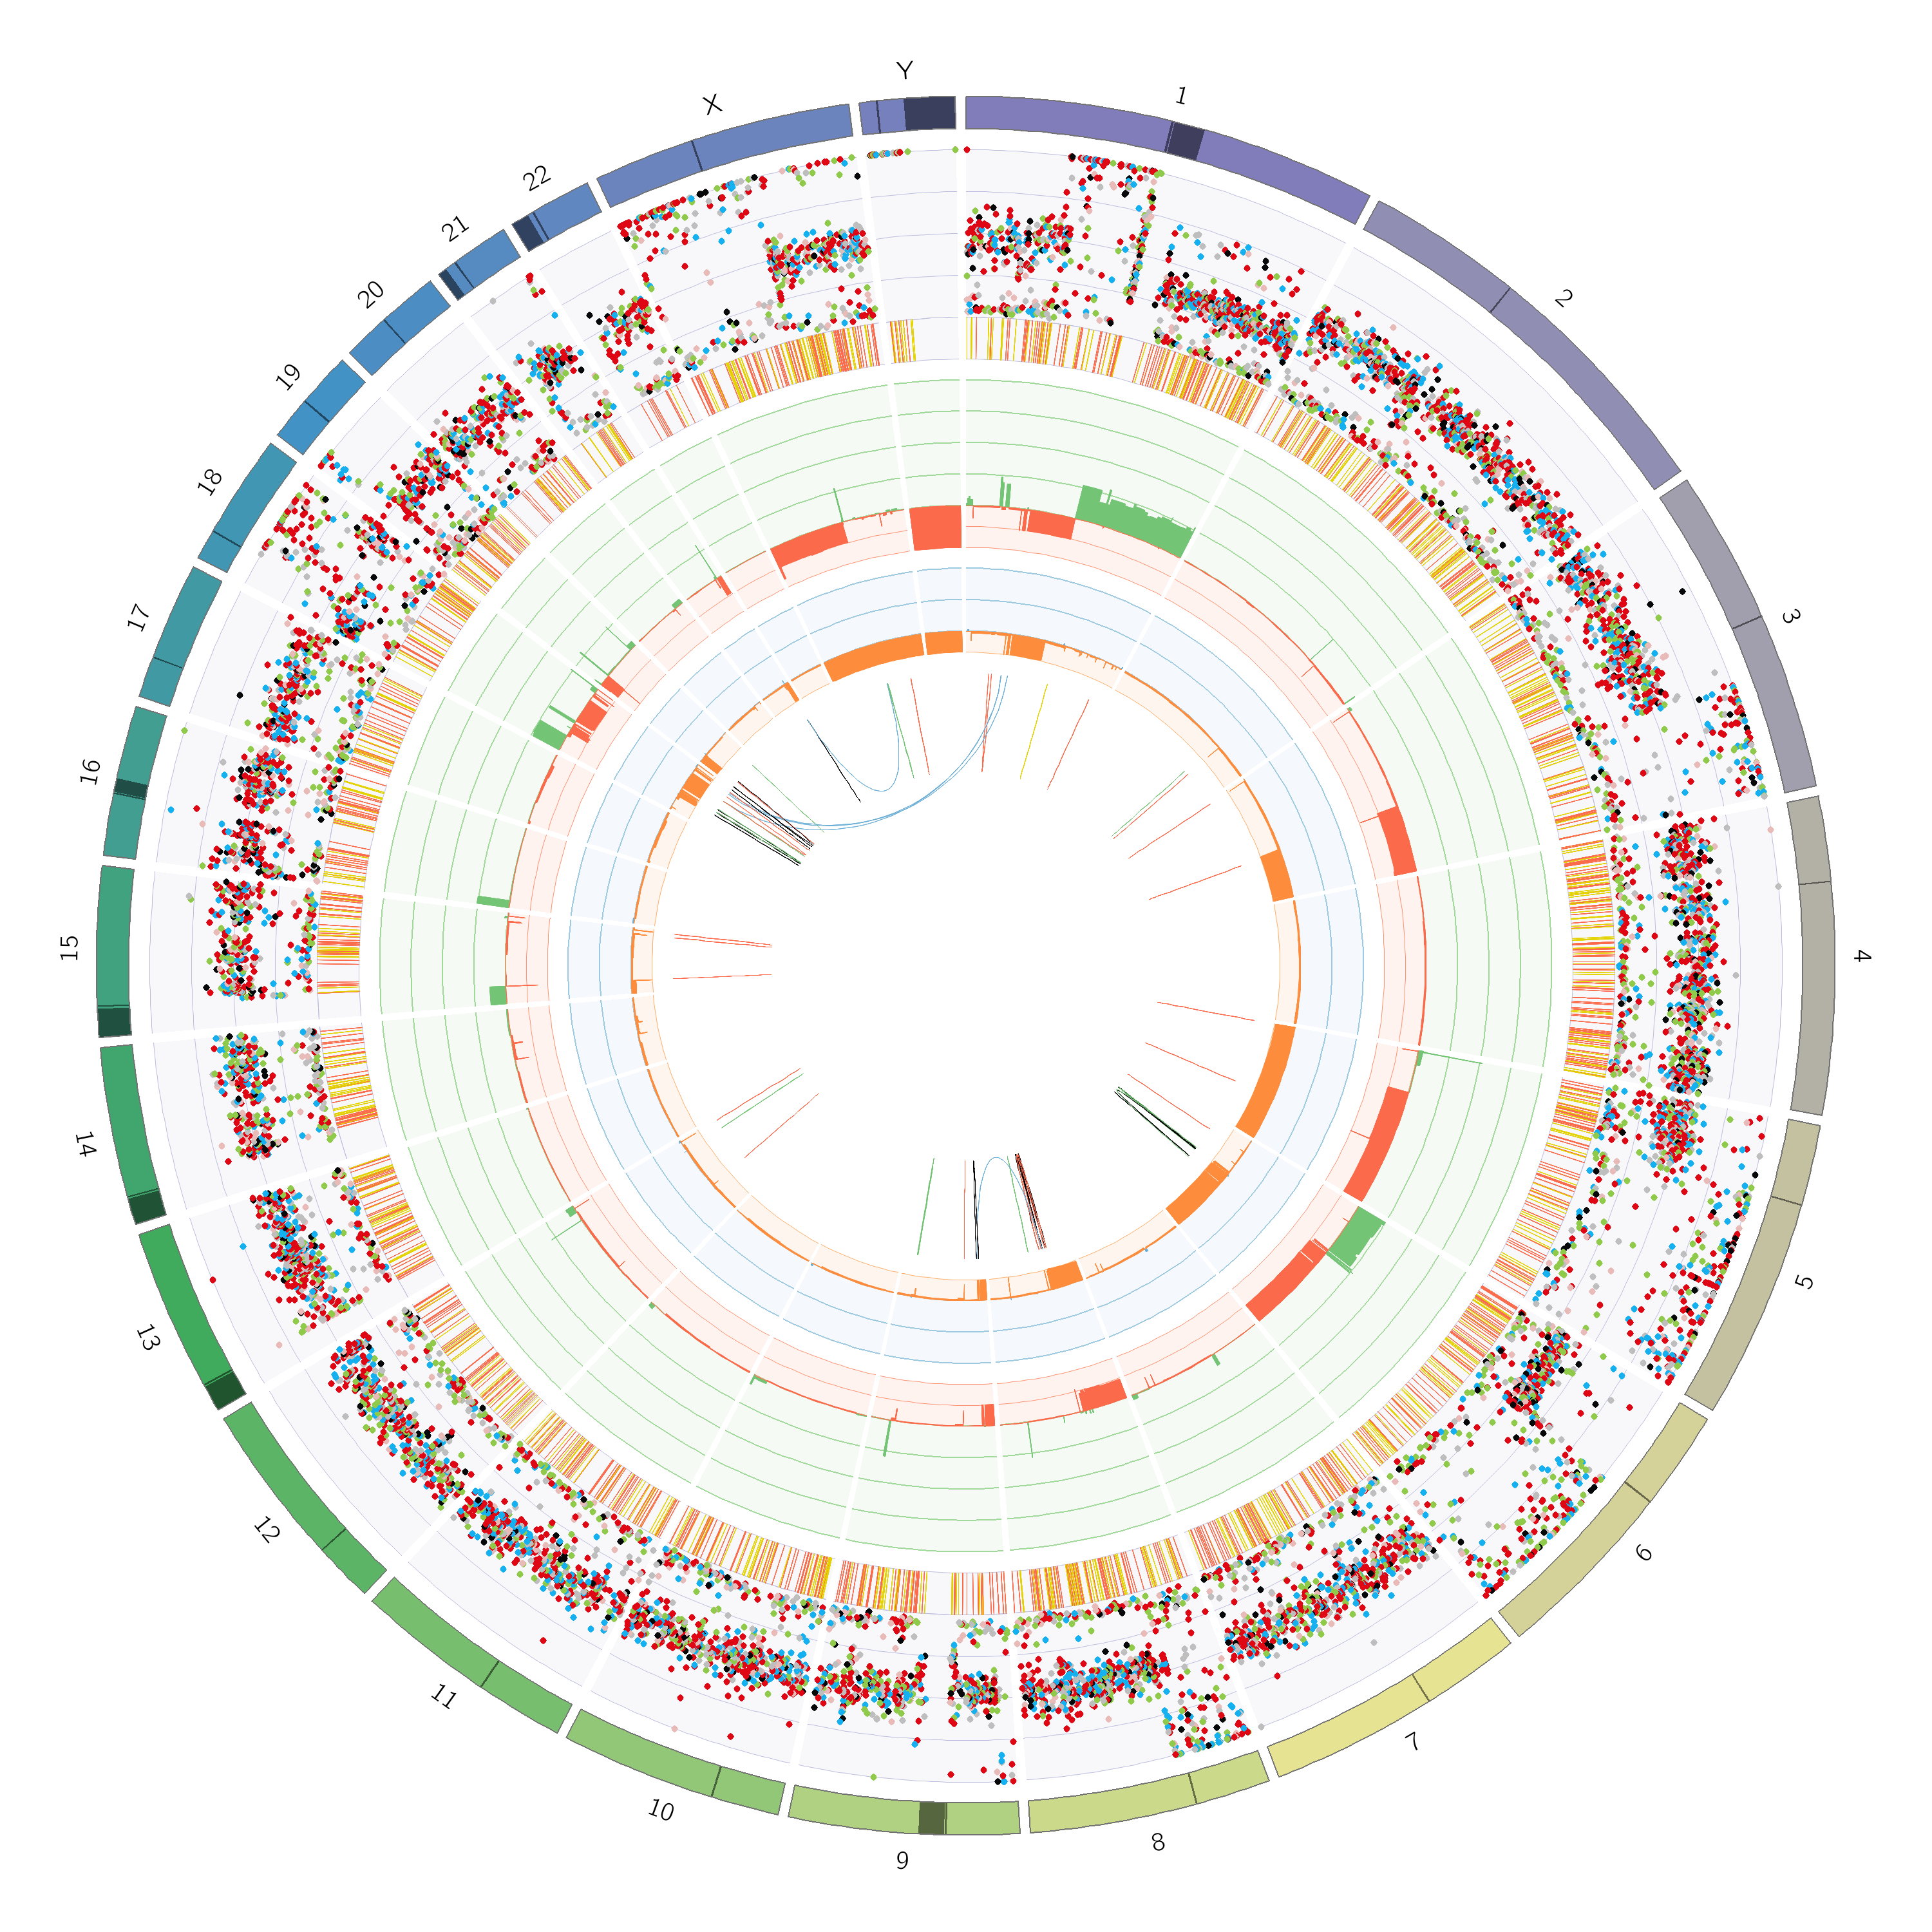
\includegraphics[width=.99\linewidth]{Figures/CASCADE/CA82/CA82-5.circos.png}
\caption[Circos plot of patient CA-K sample 5]{Circos plot of patient CA-K sample 5: outer first ring shows the canonical chromosomes with gaps (centromere, heterochromatin,...) highlighted as darker areas; second ring visualises all somatic SNVs corrected for tumour purity and scaled from 0 to 1, the colour representing the base change of SNV like in \protect\textcite{Alexandrov2013}; vertical lines directly under the SNVs symbolise InDels, with yellow for insertions and red for deletions; the third ring shows the total copy number alterations, with green showing a copy number gain and red a loss, dots at the outer border show a copy number greater than four; the last ring shows the minor copy number, with blue depicting a gain and orange a loss, this ring allows the detection of copy number neutral changes, like loss of heterozygosity; the center shows all structural variants: translocations in blue, deletions in red, insertions in yellow, tandem duplications in green and inversions in black.} \label{fig:ca82.5circos}
\end{figure}

\begin{figure}[ht]
\centering
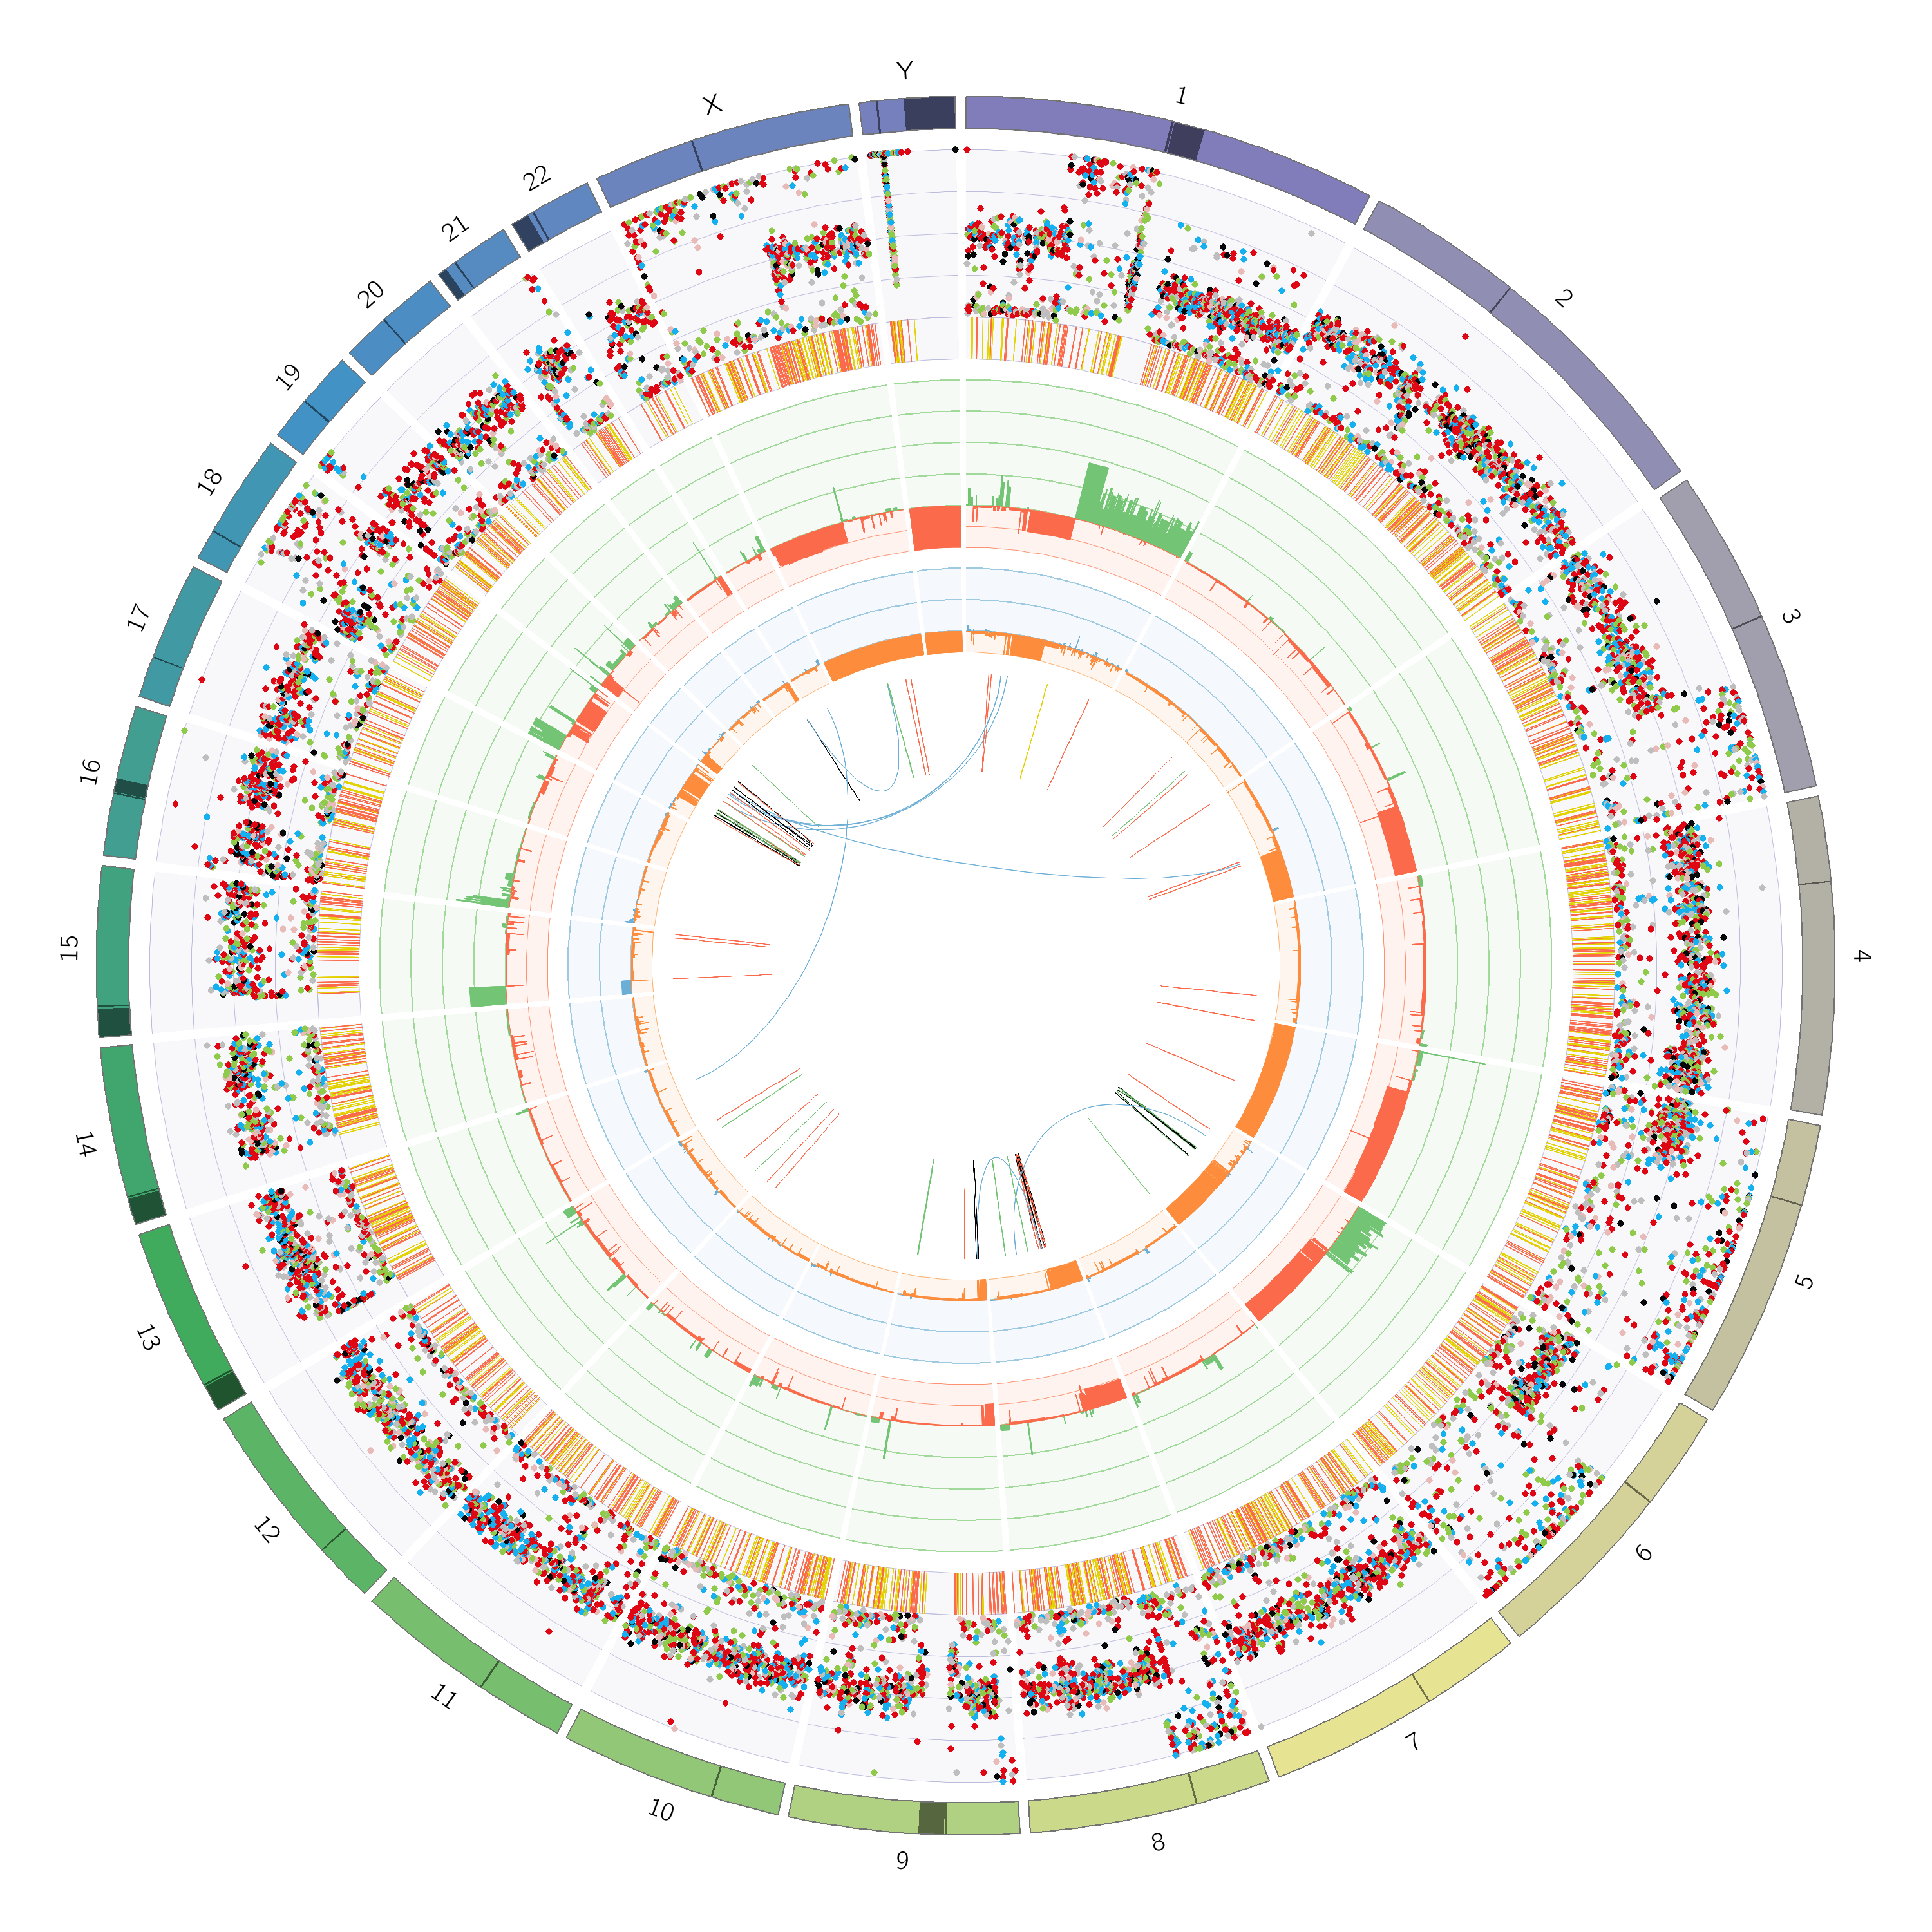
\includegraphics[width=.99\linewidth]{Figures/CASCADE/CA82/CA82-6.circos.png}
\caption[Circos plot of patient CA-K sample 6]{Circos plot of patient CA-K sample 6: outer first ring shows the canonical chromosomes with gaps (centromere, heterochromatin,...) highlighted as darker areas; second ring visualises all somatic SNVs corrected for tumour purity and scaled from 0 to 1, the colour representing the base change of SNV like in \protect\textcite{Alexandrov2013}; vertical lines directly under the SNVs symbolise InDels, with yellow for insertions and red for deletions; the third ring shows the total copy number alterations, with green showing a copy number gain and red a loss, dots at the outer border show a copy number greater than four; the last ring shows the minor copy number, with blue depicting a gain and orange a loss, this ring allows the detection of copy number neutral changes, like loss of heterozygosity; the center shows all structural variants: translocations in blue, deletions in red, insertions in yellow, tandem duplications in green and inversions in black.} \label{fig:ca82.6circos}
\end{figure}

\begin{figure}[ht]
\centering
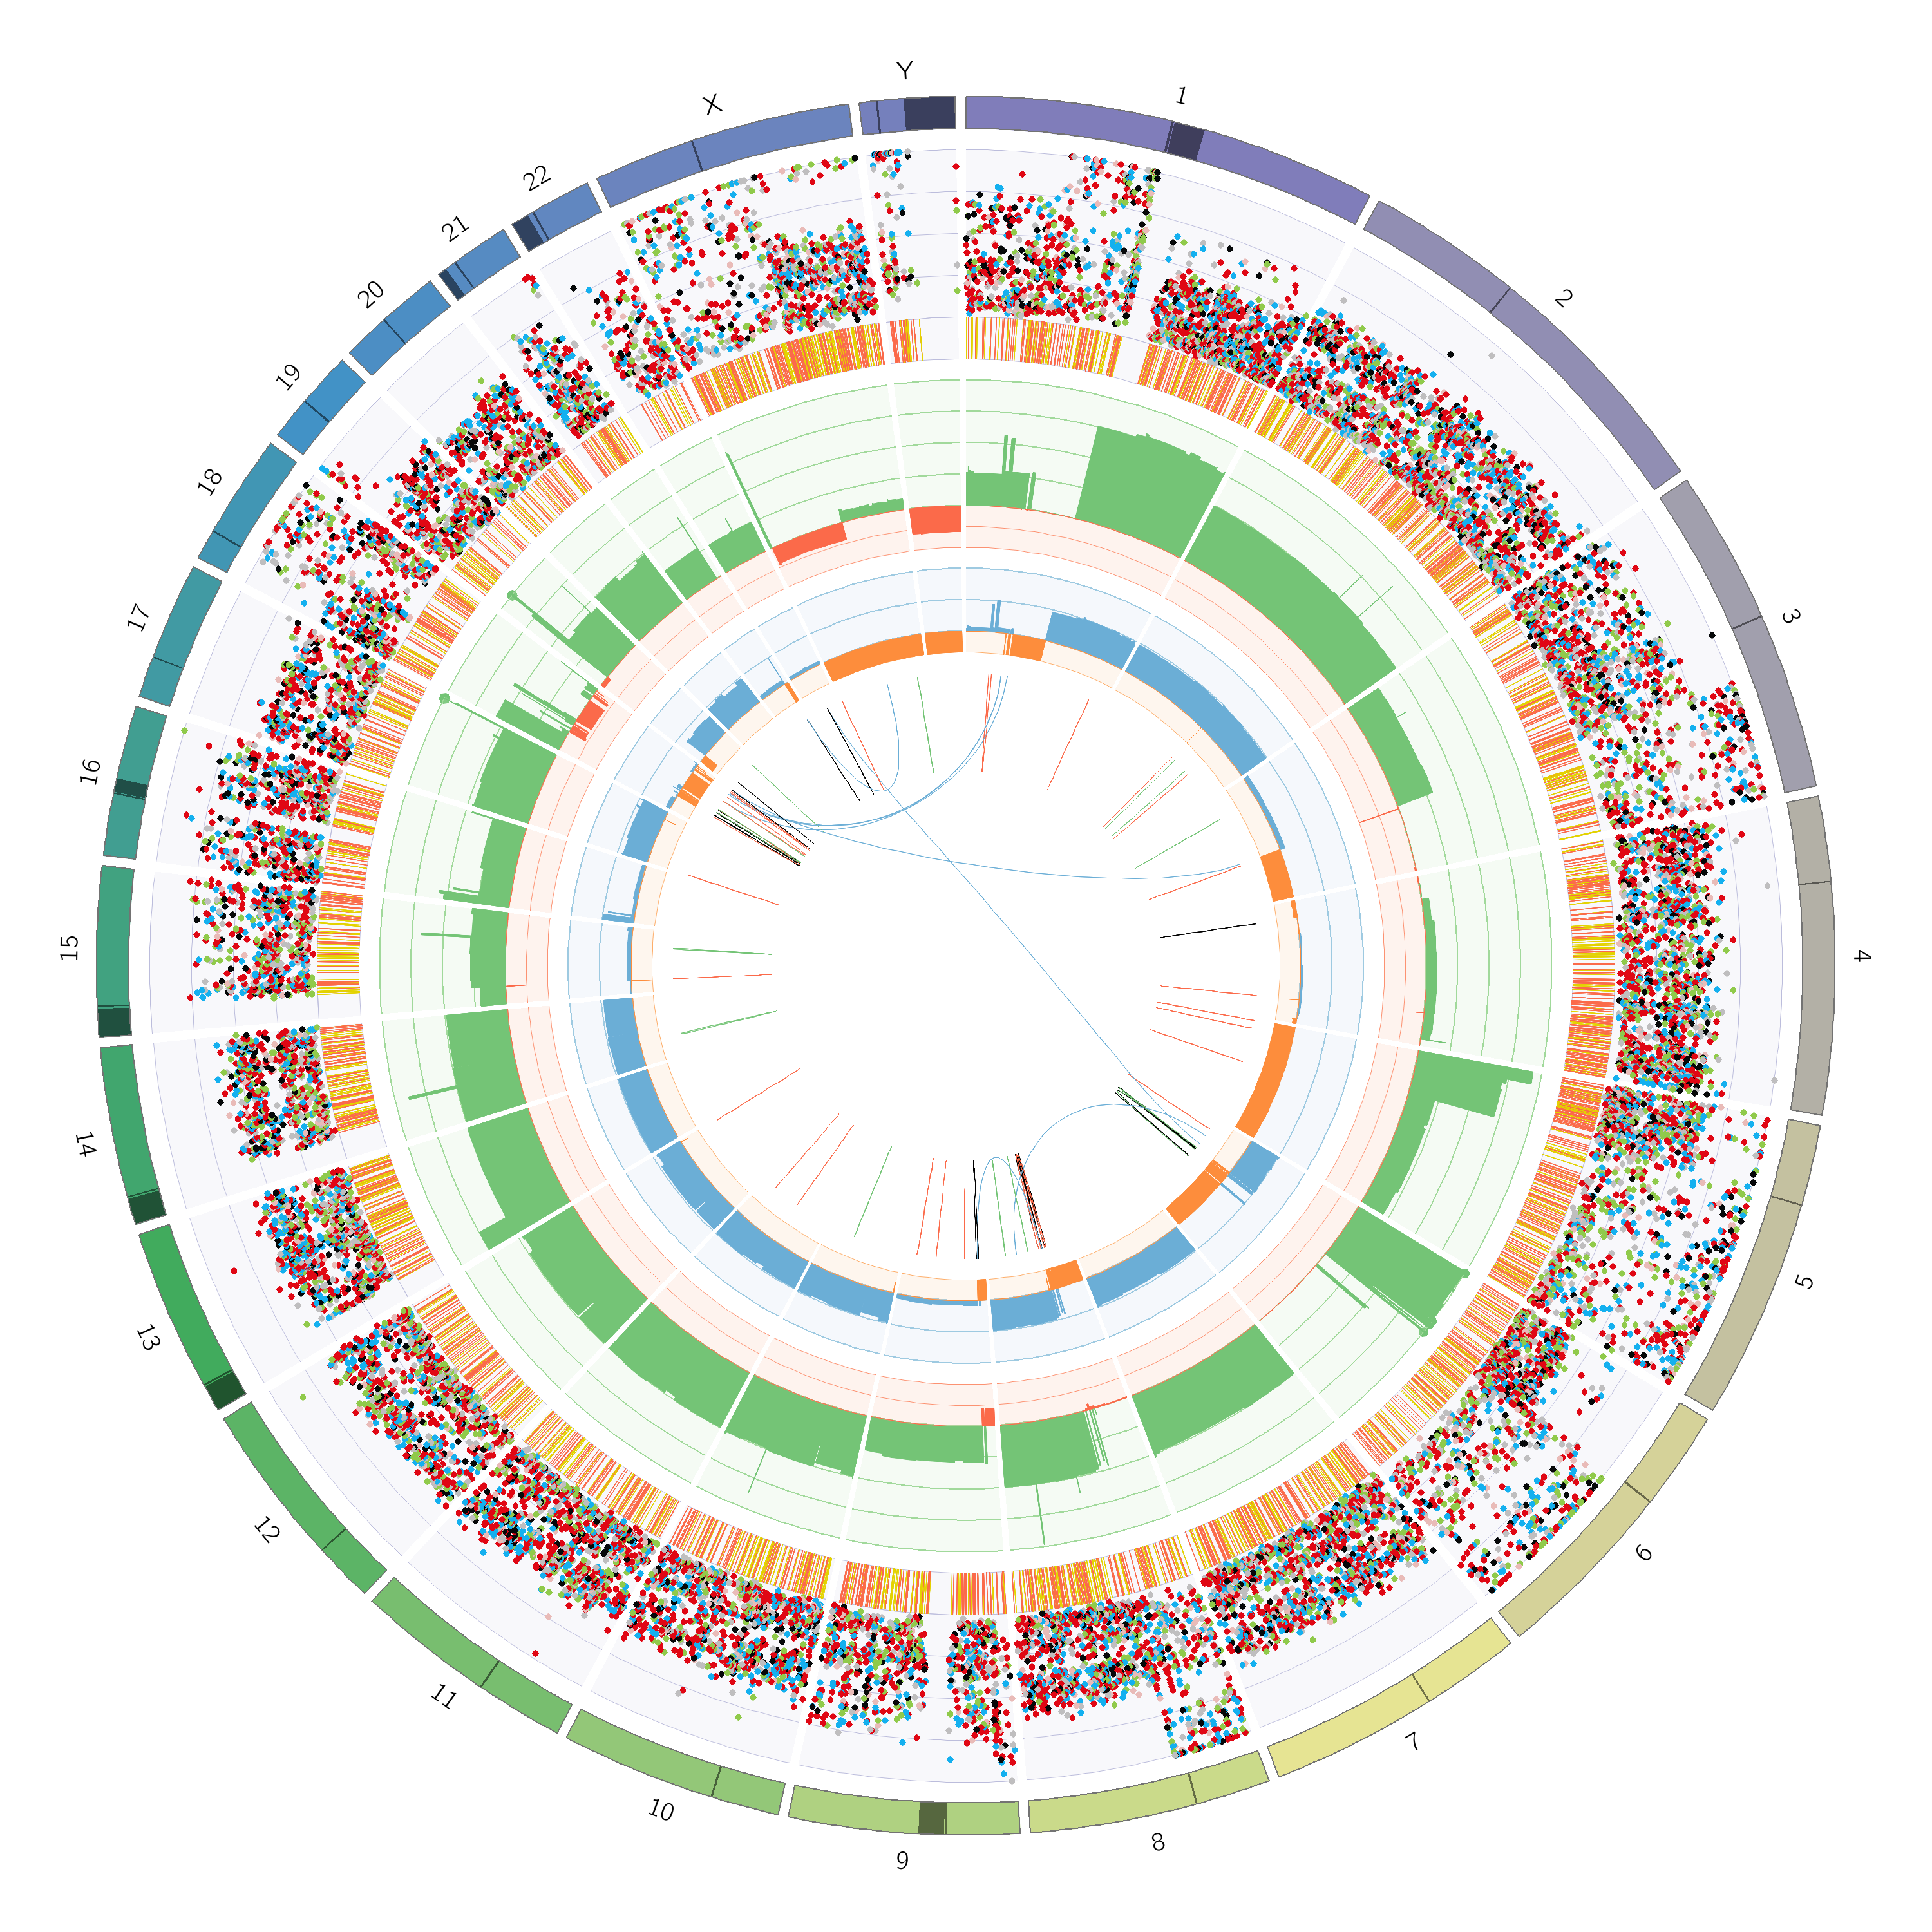
\includegraphics[width=.99\linewidth]{Figures/CASCADE/CA82/CA82-9.circos.png}
\caption[Circos plot of patient CA-K sample 9]{Circos plot of patient CA-K sample 9: outer first ring shows the canonical chromosomes with gaps (centromere, heterochromatin,...) highlighted as darker areas; second ring visualises all somatic SNVs corrected for tumour purity and scaled from 0 to 1, the colour representing the base change of SNV like in \protect\textcite{Alexandrov2013}; vertical lines directly under the SNVs symbolise InDels, with yellow for insertions and red for deletions; the third ring shows the total copy number alterations, with green showing a copy number gain and red a loss, dots at the outer border show a copy number greater than four; the last ring shows the minor copy number, with blue depicting a gain and orange a loss, this ring allows the detection of copy number neutral changes, like loss of heterozygosity; the center shows all structural variants: translocations in blue, deletions in red, insertions in yellow, tandem duplications in green and inversions in black.} \label{fig:ca82.9circos}
\end{figure}

\begin{figure}[ht]
\centering
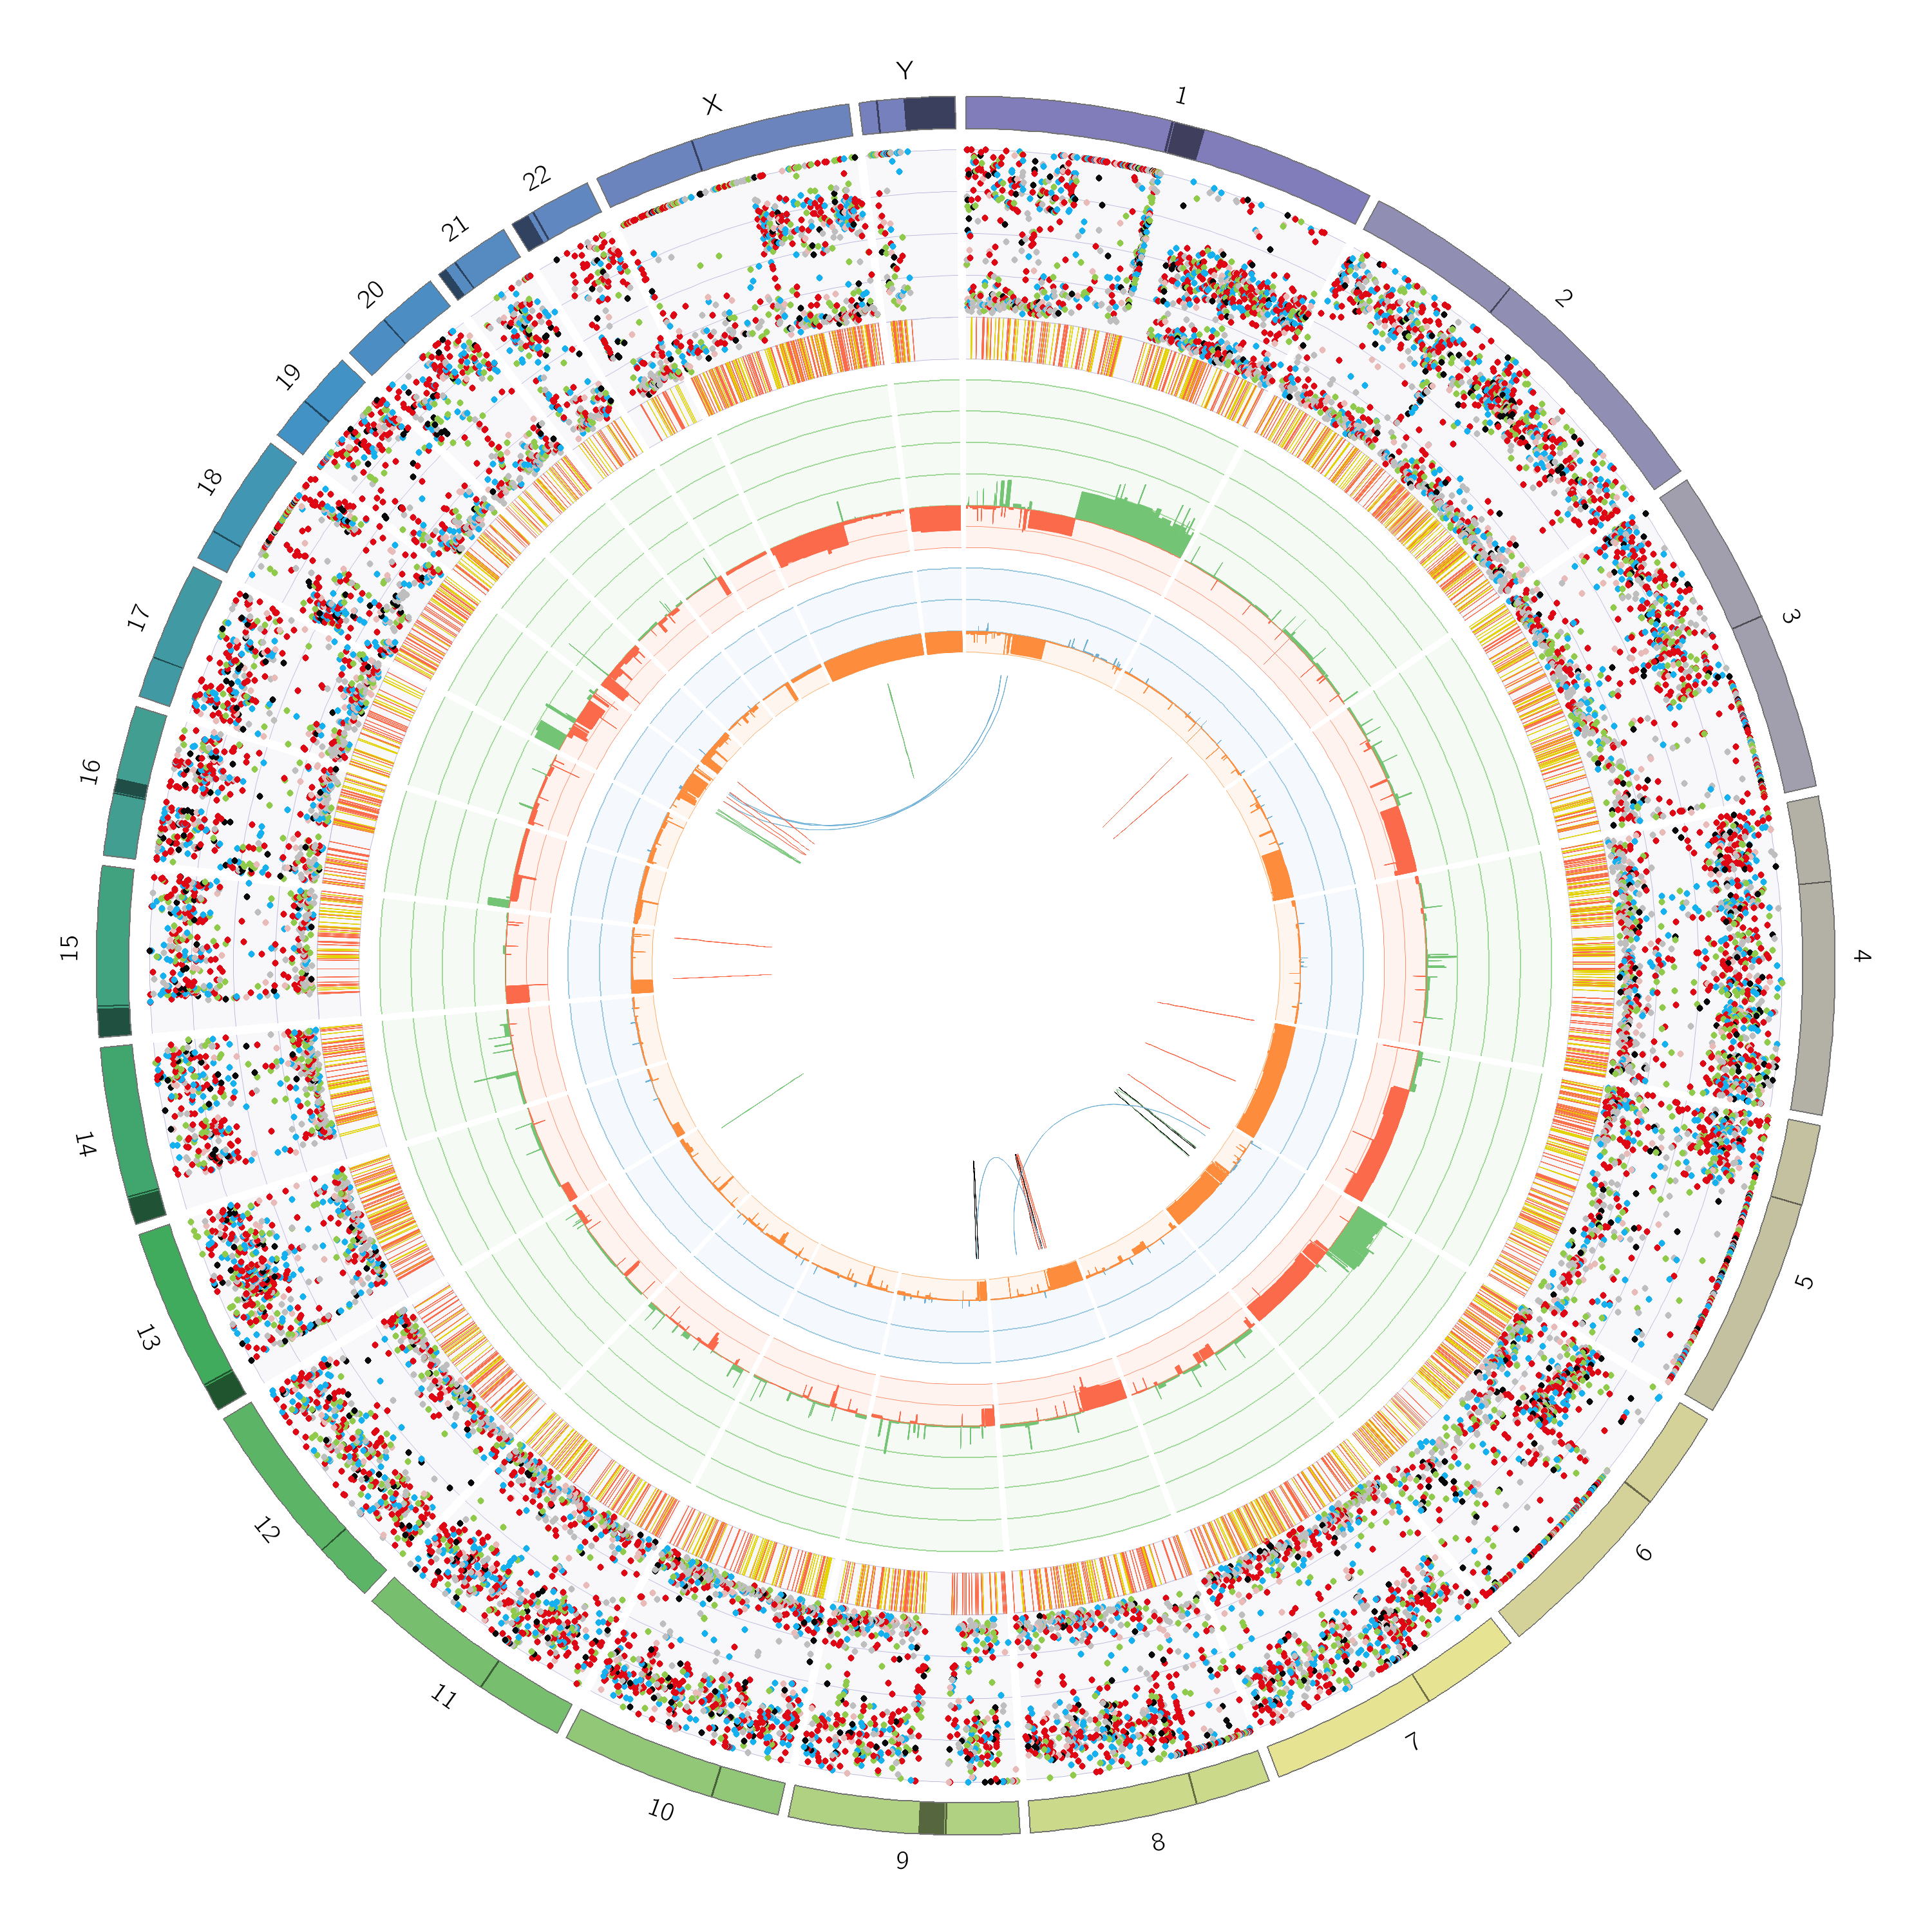
\includegraphics[width=.99\linewidth]{Figures/CASCADE/CA82/CA82-13.circos.png}
\caption[Circos plot of patient CA-K sample 13]{Circos plot of patient CA-K sample 13: outer first ring shows the canonical chromosomes with gaps (centromere, heterochromatin,...) highlighted as darker areas; second ring visualises all somatic SNVs corrected for tumour purity and scaled from 0 to 1, the colour representing the base change of SNV like in \protect\textcite{Alexandrov2013}; vertical lines directly under the SNVs symbolise InDels, with yellow for insertions and red for deletions; the third ring shows the total copy number alterations, with green showing a copy number gain and red a loss, dots at the outer border show a copy number greater than four; the last ring shows the minor copy number, with blue depicting a gain and orange a loss, this ring allows the detection of copy number neutral changes, like loss of heterozygosity; the center shows all structural variants: translocations in blue, deletions in red, insertions in yellow, tandem duplications in green and inversions in black.} \label{fig:ca82.13circos}
\end{figure}




\cleardoublepage
\subsection{Patient CA-L}

\begin{figure}[ht]
\centering
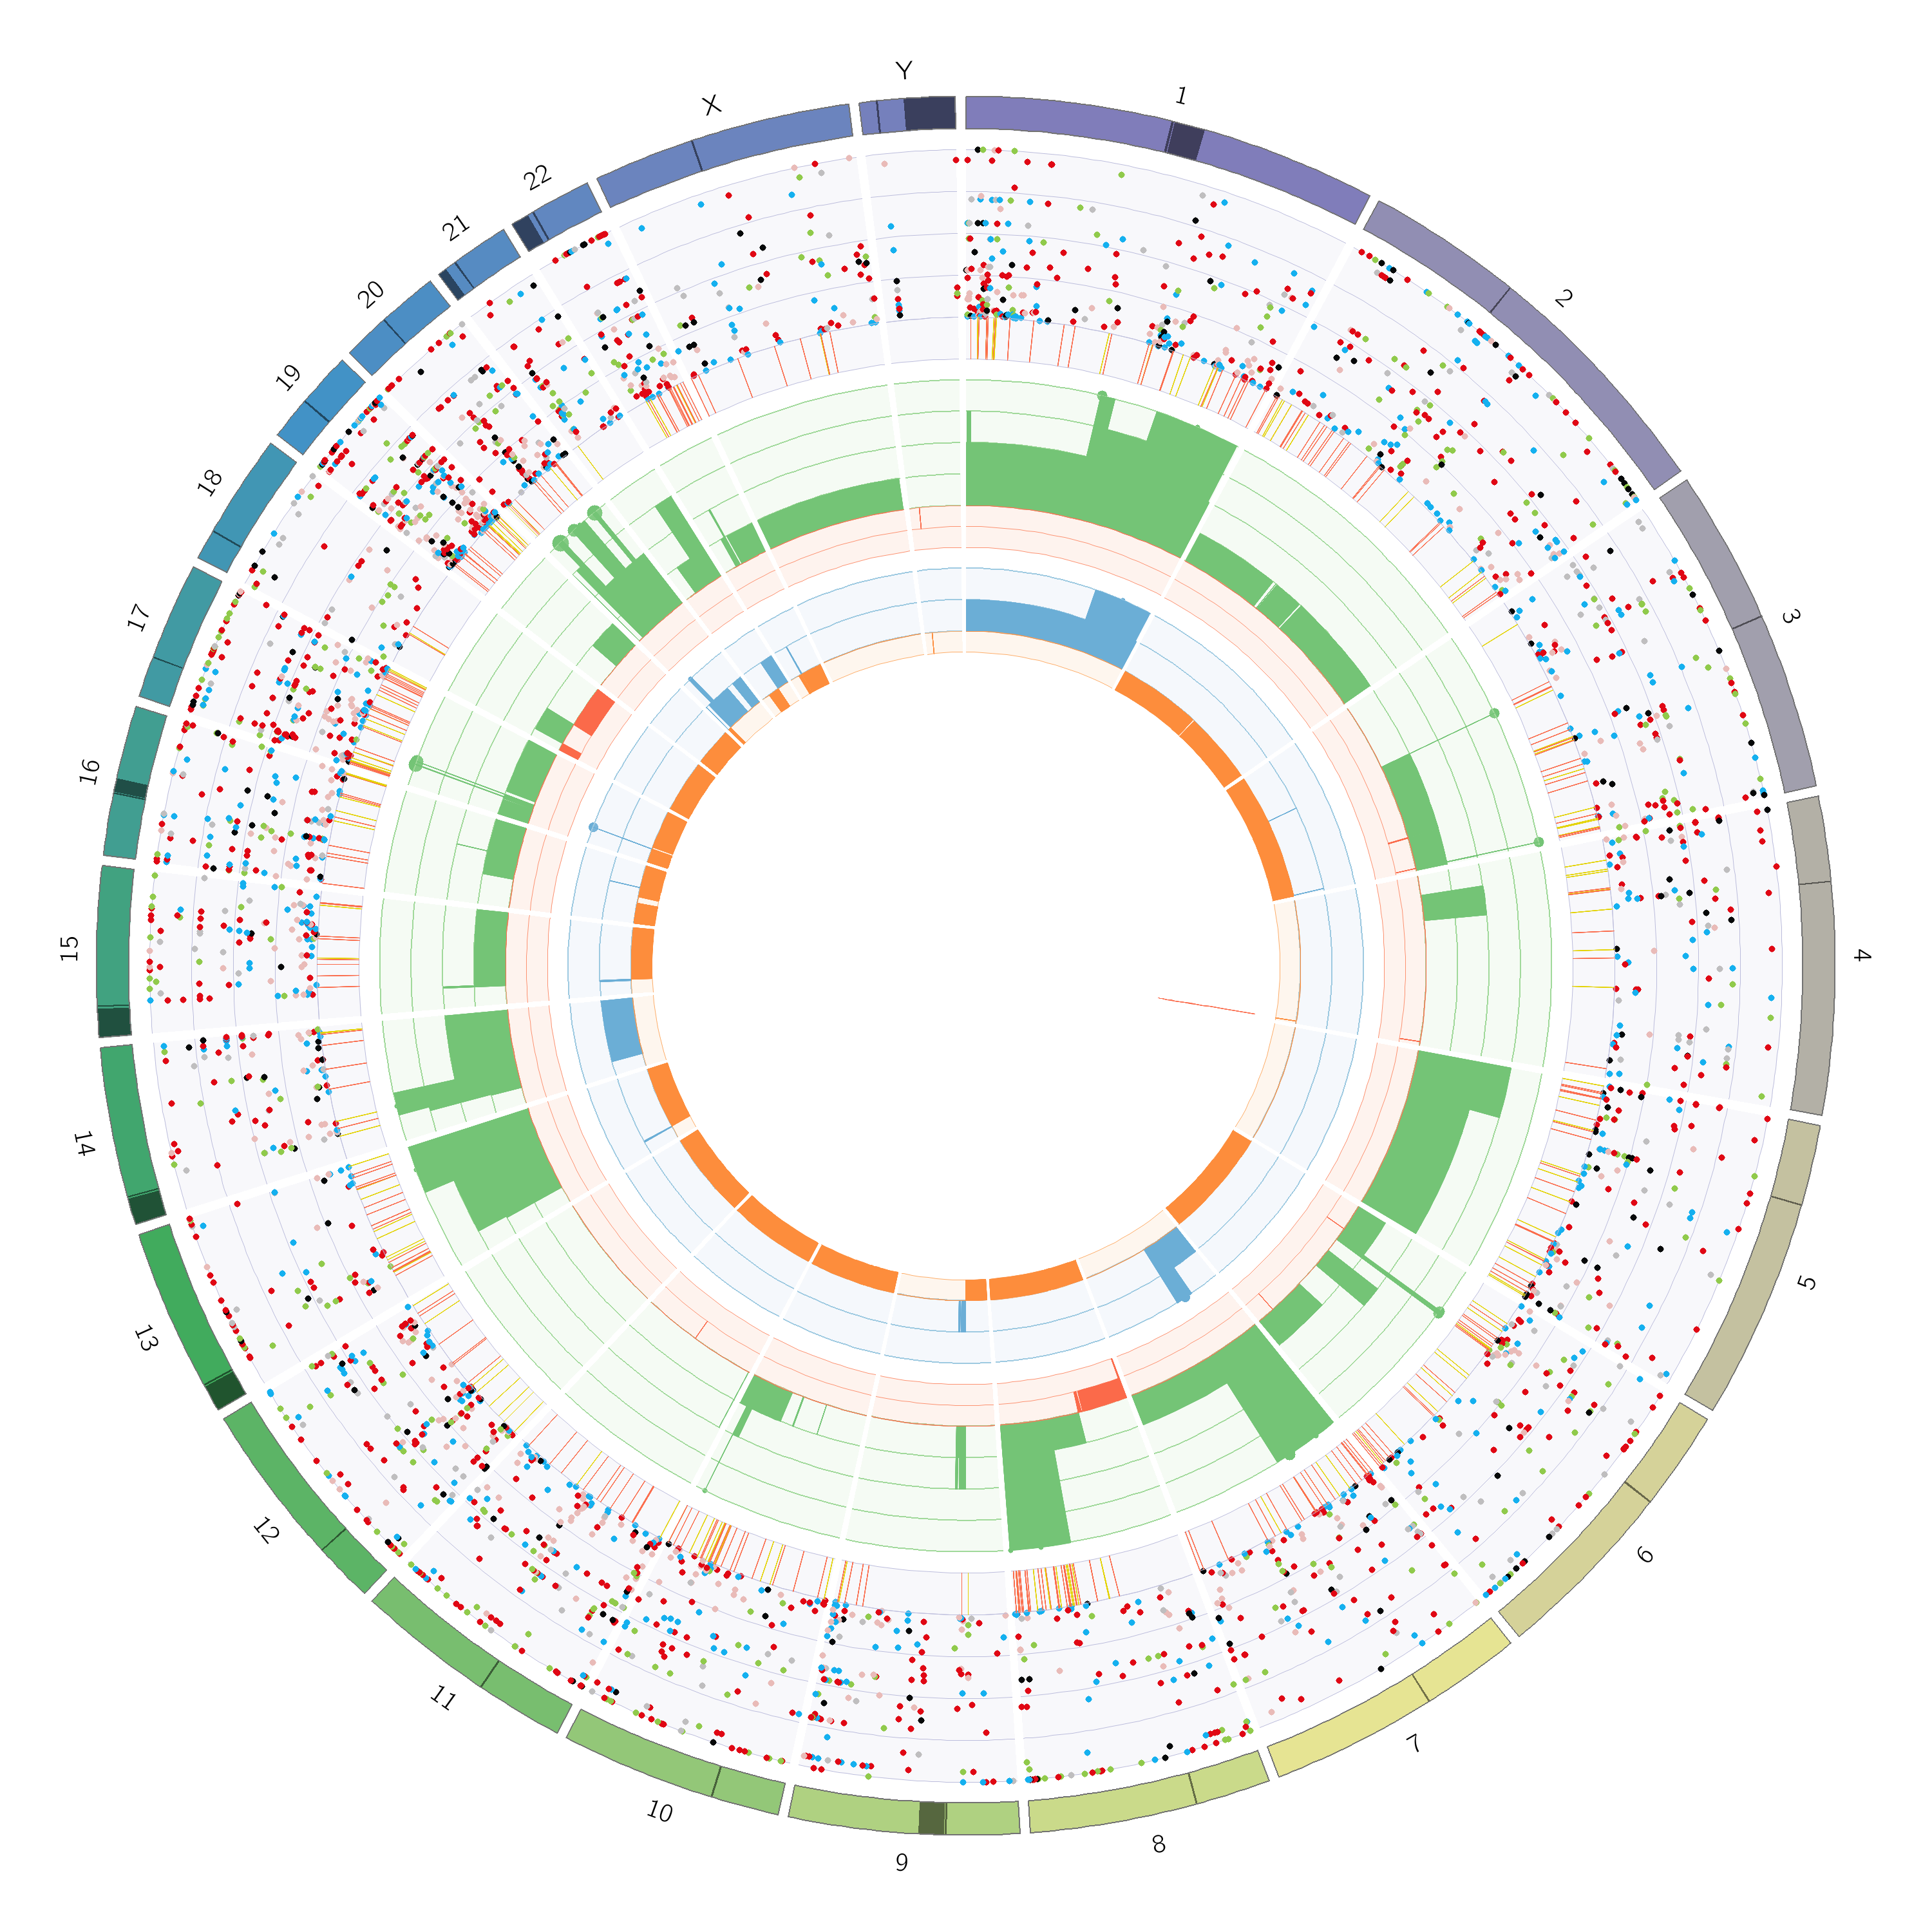
\includegraphics[width=.99\linewidth]{Figures/CASCADE/CA86/CA86-8.circos.png}
\caption[Circos plot of patient CA-L sample 8]{Circos plot of patient CA-L sample 8: outer first ring shows the canonical chromosomes with gaps (centromere, heterochromatin,...) highlighted as darker areas; second ring visualises all somatic SNVs corrected for tumour purity and scaled from 0 to 1, the colour representing the base change of SNV like in \protect\textcite{Alexandrov2013}; vertical lines directly under the SNVs symbolise InDels, with yellow for insertions and red for deletions; the third ring shows the total copy number alterations, with green showing a copy number gain and red a loss, dots at the outer border show a copy number greater than four; the last ring shows the minor copy number, with blue depicting a gain and orange a loss, this ring allows the detection of copy number neutral changes, like loss of heterozygosity; the center shows all structural variants: translocations in blue, deletions in red, insertions in yellow, tandem duplications in green and inversions in black.} \label{fig:ca86.8circos}
\end{figure}


\begin{figure}[ht]
\centering
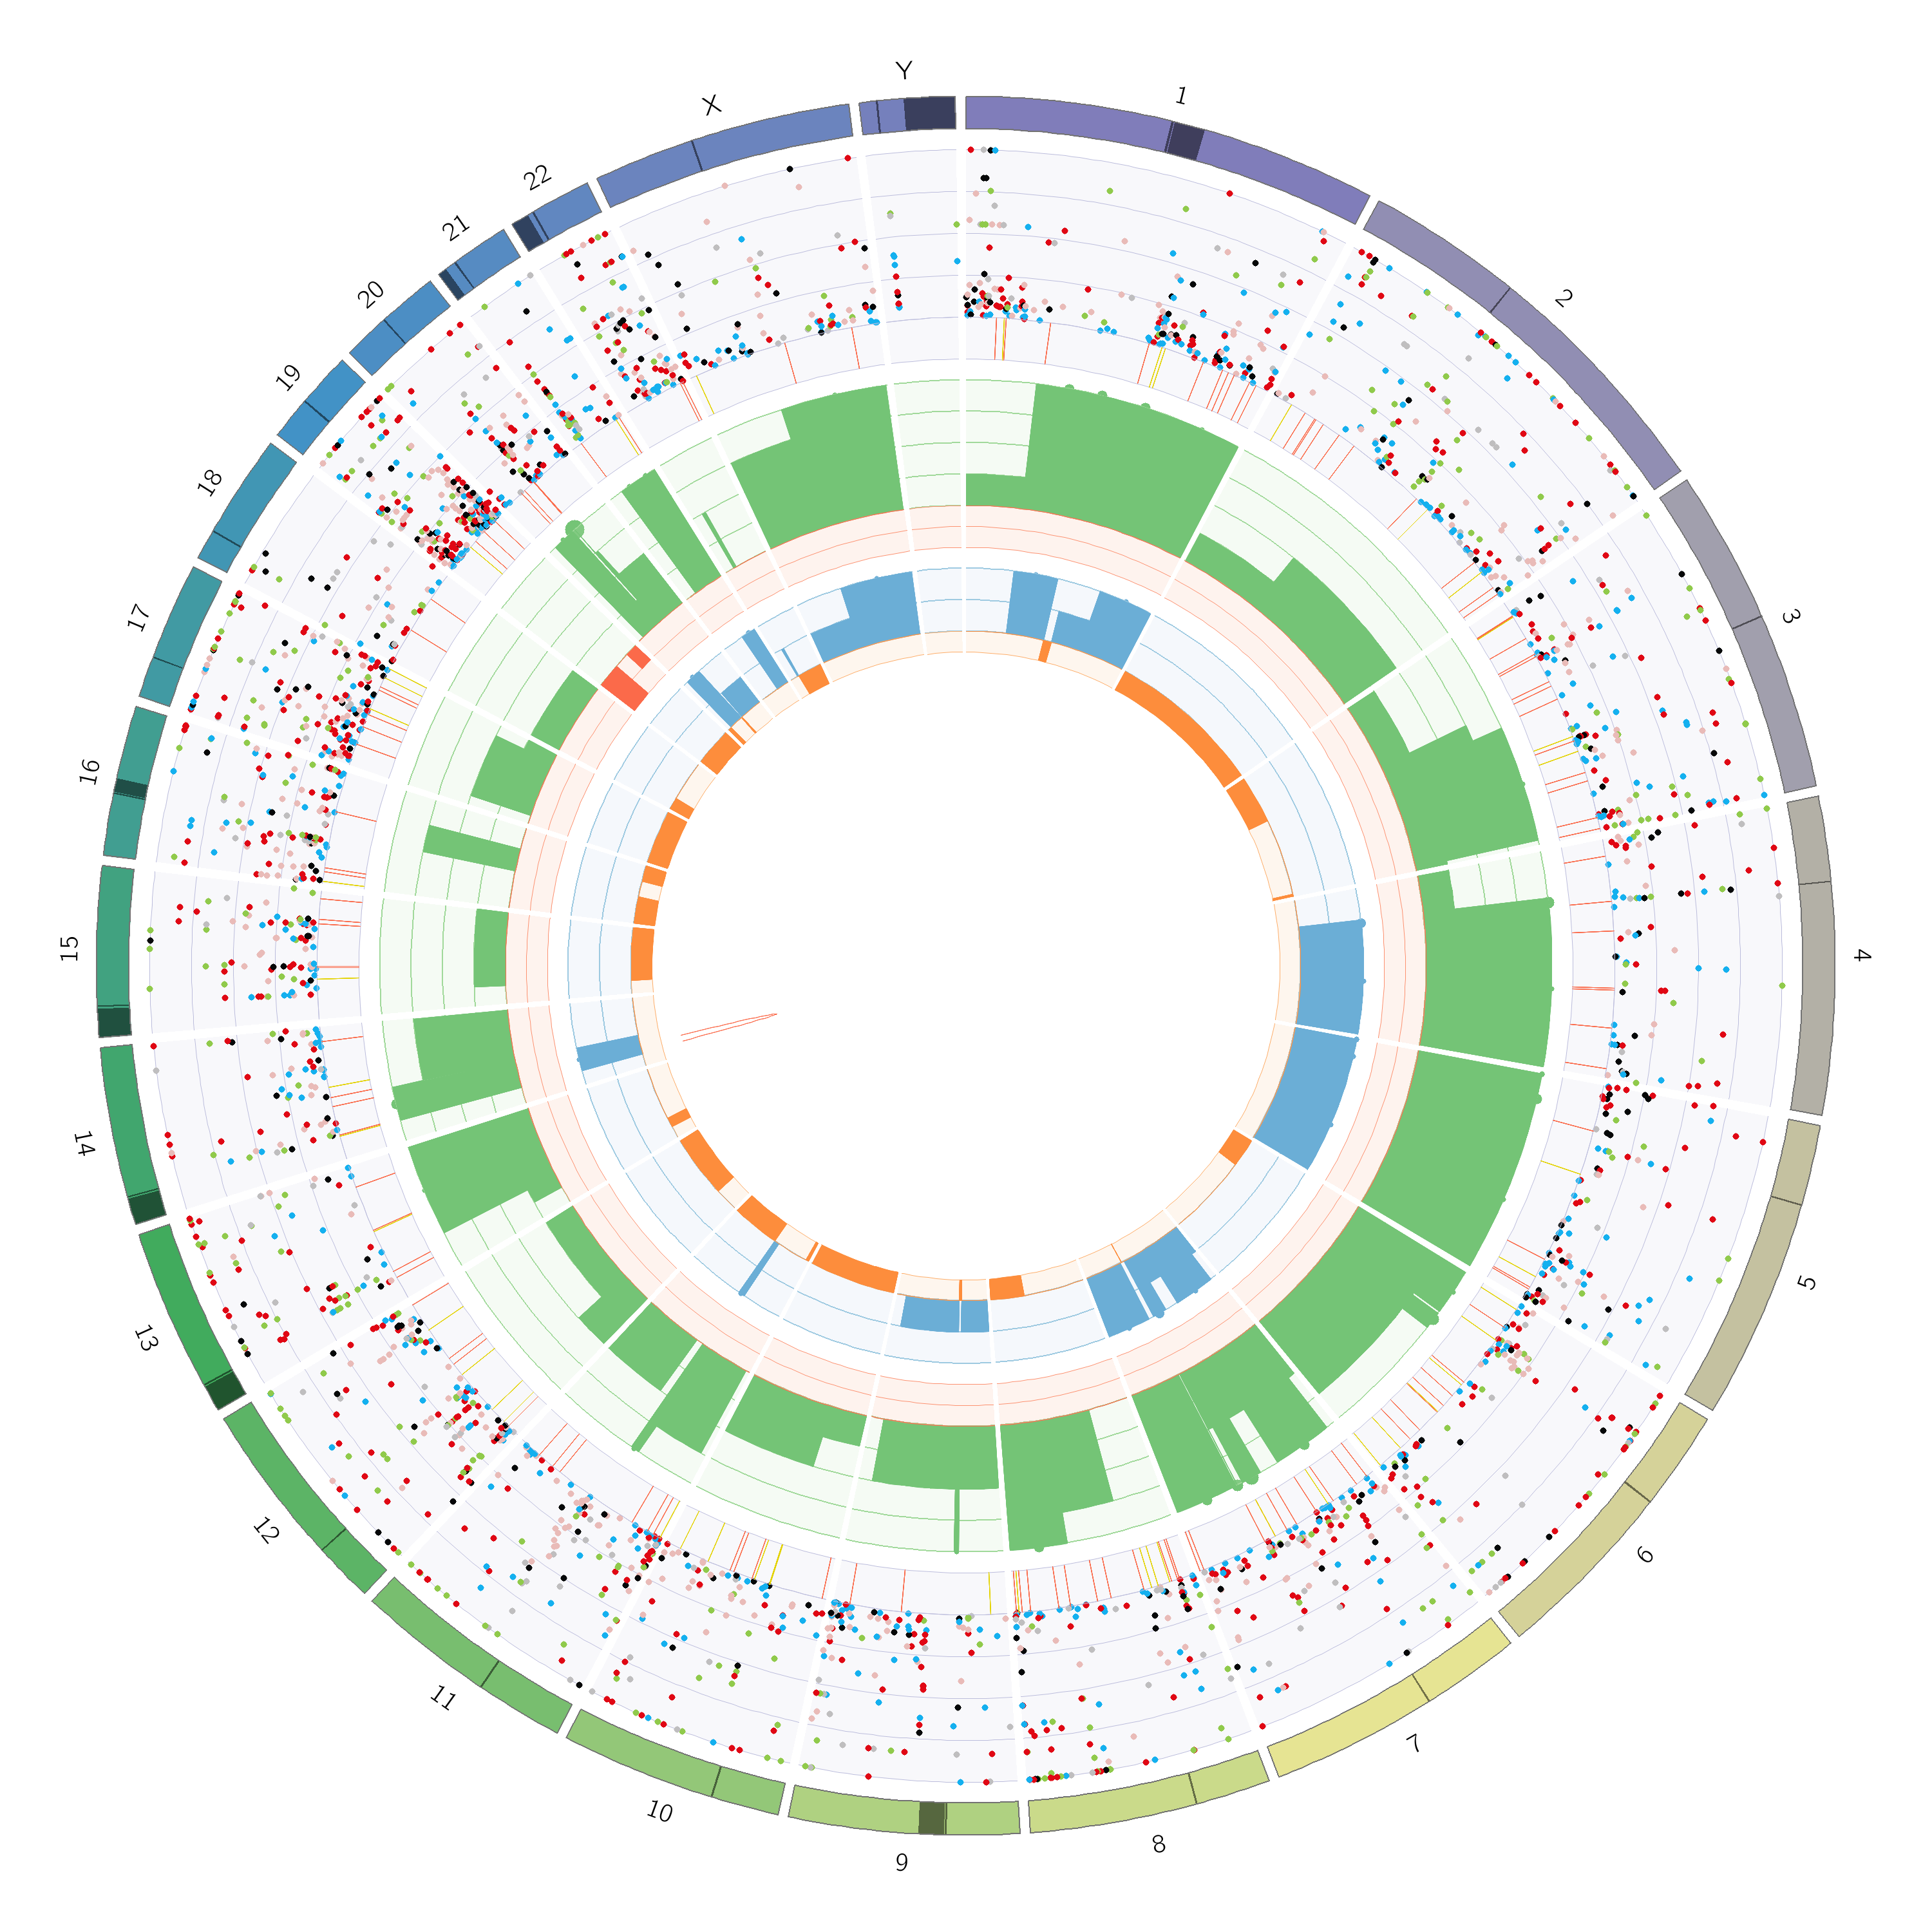
\includegraphics[width=.99\linewidth]{Figures/CASCADE/CA86/CA86-17A.circos.png}
\caption[Circos plot of patient CA-L sample 17A]{Circos plot of patient CA-L sample 17A: outer first ring shows the canonical chromosomes with gaps (centromere, heterochromatin,...) highlighted as darker areas; second ring visualises all somatic SNVs corrected for tumour purity and scaled from 0 to 1, the colour representing the base change of SNV like in \protect\textcite{Alexandrov2013}; vertical lines directly under the SNVs symbolise InDels, with yellow for insertions and red for deletions; the third ring shows the total copy number alterations, with green showing a copy number gain and red a loss, dots at the outer border show a copy number greater than four; the last ring shows the minor copy number, with blue depicting a gain and orange a loss, this ring allows the detection of copy number neutral changes, like loss of heterozygosity; the center shows all structural variants: translocations in blue, deletions in red, insertions in yellow, tandem duplications in green and inversions in black.} \label{fig:ca86.17Acircos}
\end{figure}


\begin{figure}[ht]
\centering
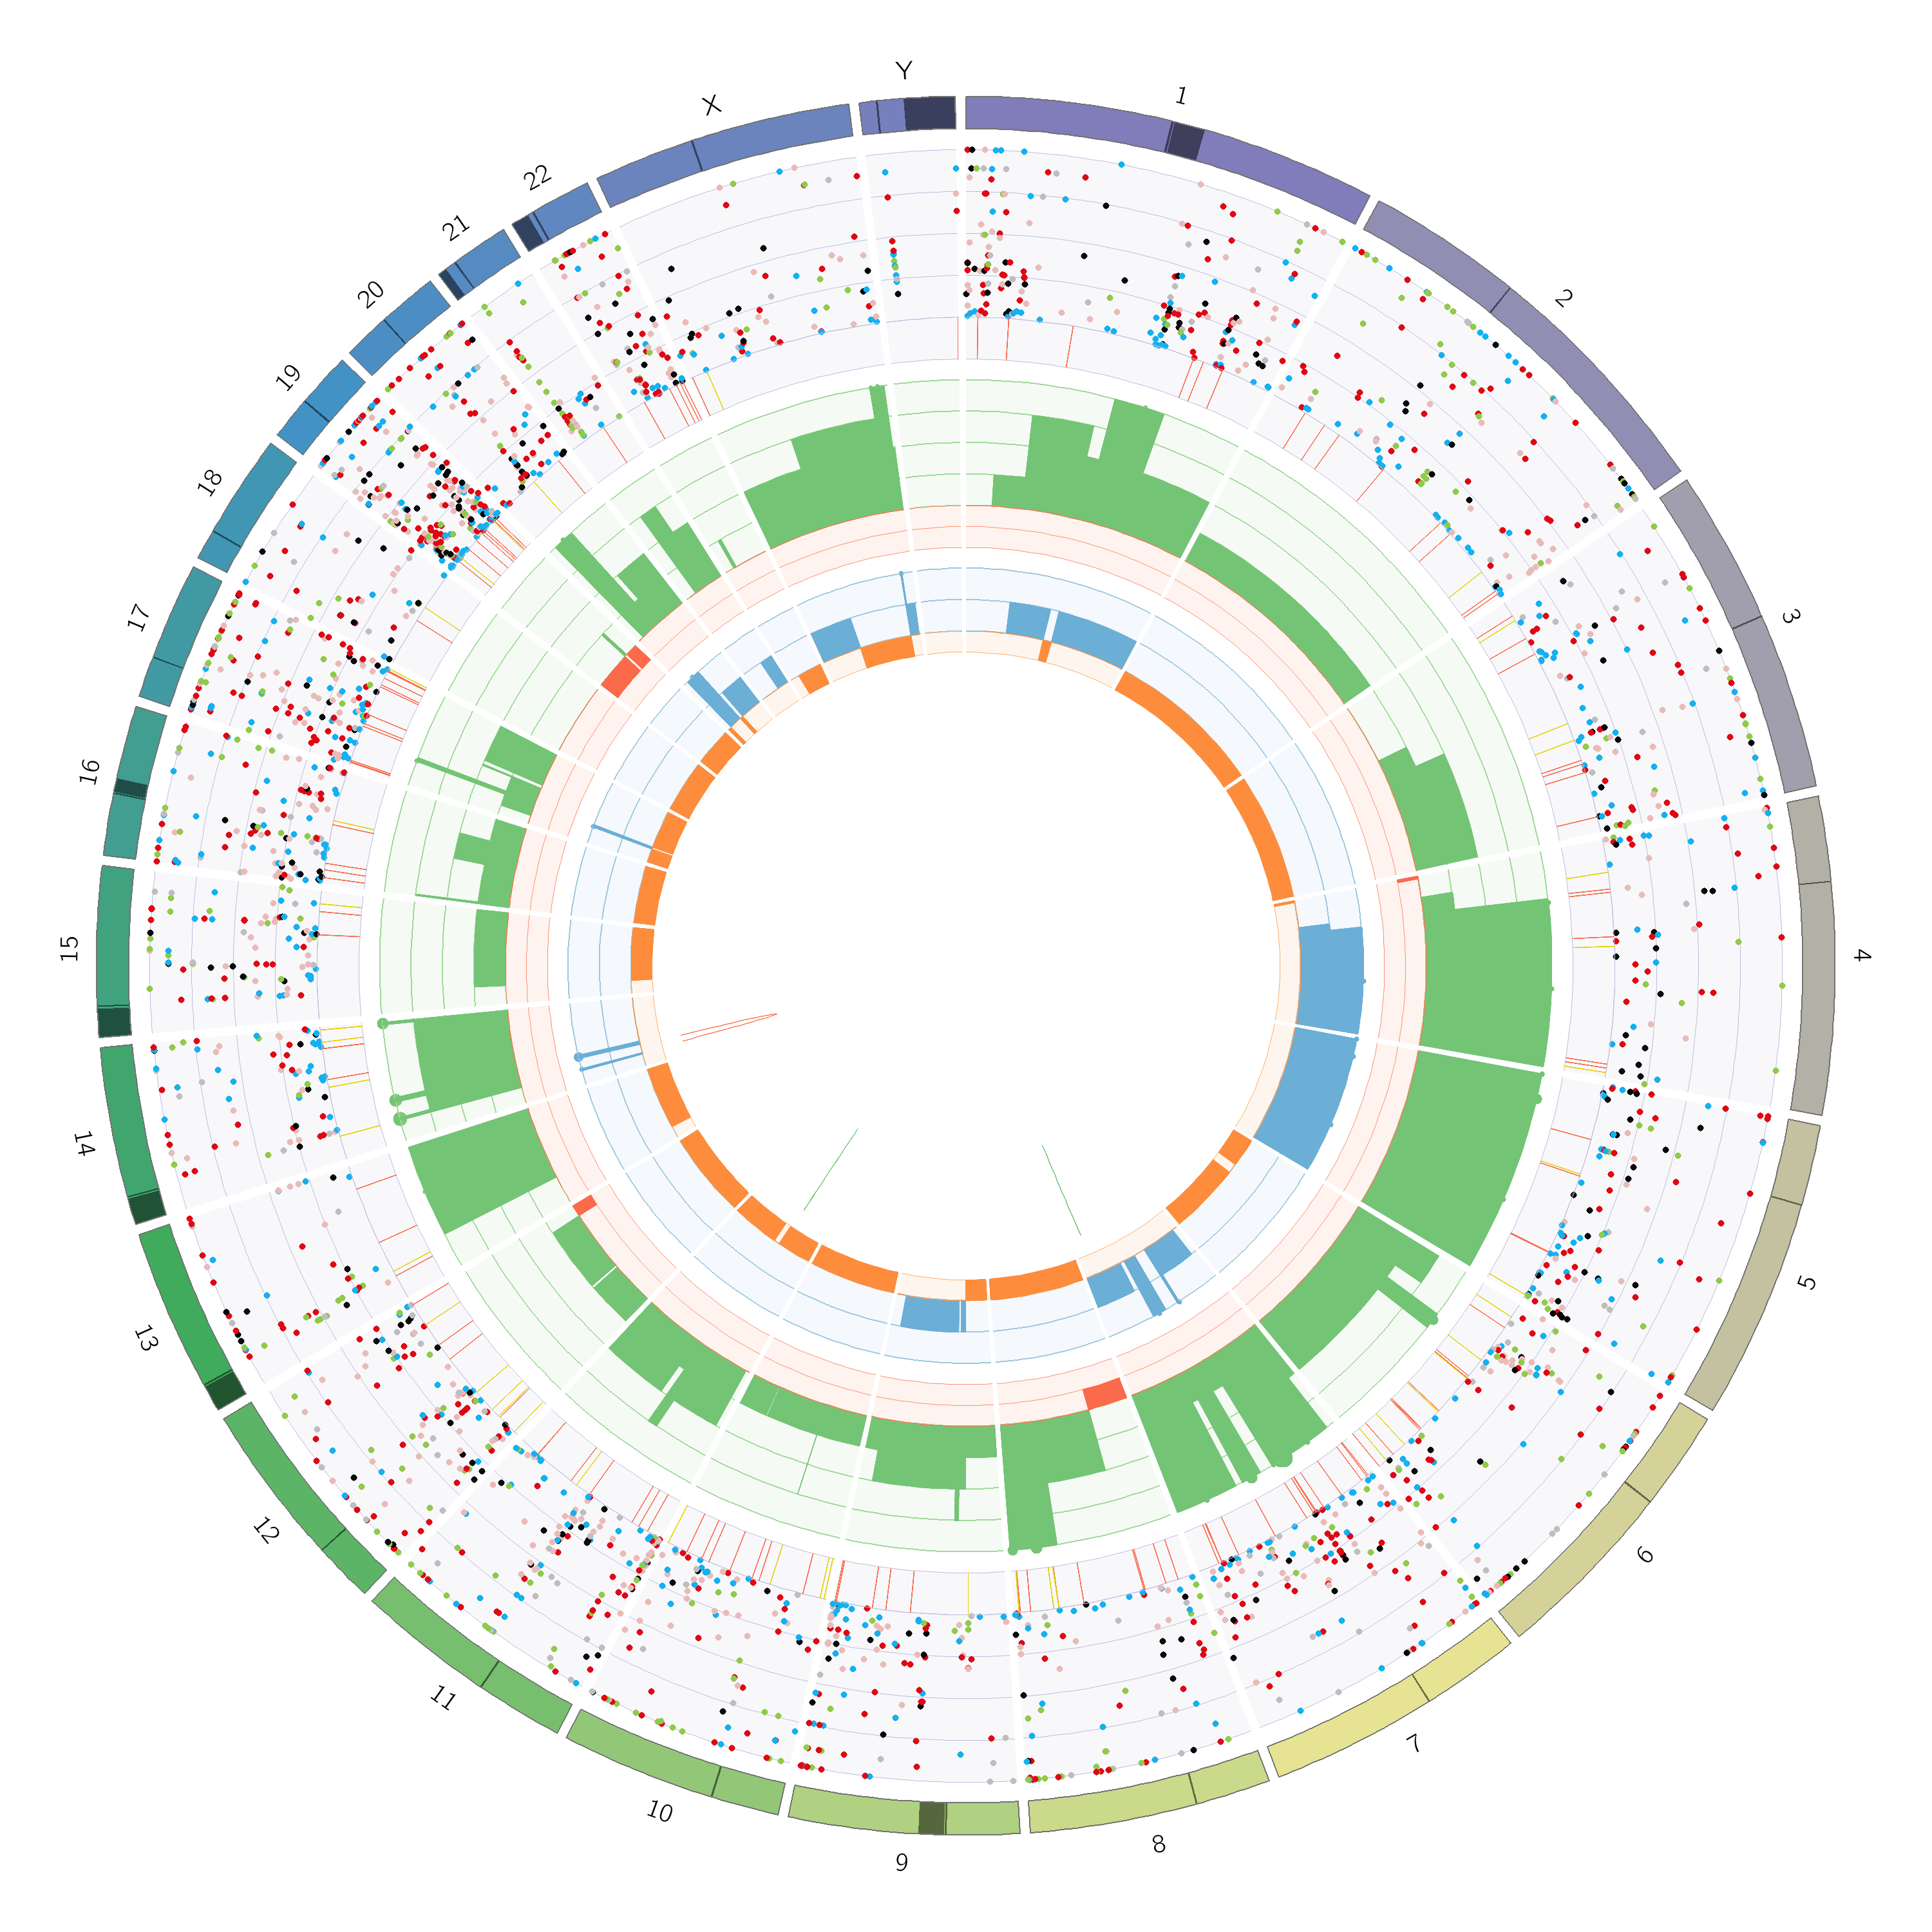
\includegraphics[width=.99\linewidth]{Figures/CASCADE/CA86/CA86-26.circos.png}
\caption[Circos plot of patient CA-L sample 26]{Circos plot of patient CA-L sample 26: outer first ring shows the canonical chromosomes with gaps (centromere, heterochromatin,...) highlighted as darker areas; second ring visualises all somatic SNVs corrected for tumour purity and scaled from 0 to 1, the colour representing the base change of SNV like in \protect\textcite{Alexandrov2013}; vertical lines directly under the SNVs symbolise InDels, with yellow for insertions and red for deletions; the third ring shows the total copy number alterations, with green showing a copy number gain and red a loss, dots at the outer border show a copy number greater than four; the last ring shows the minor copy number, with blue depicting a gain and orange a loss, this ring allows the detection of copy number neutral changes, like loss of heterozygosity; the center shows all structural variants: translocations in blue, deletions in red, insertions in yellow, tandem duplications in green and inversions in black.} \label{fig:ca86.26circos}
\end{figure}

